\documentclass[a4paper, 11pt]{article}

\usepackage[utf8]{inputenc}
\usepackage[T1]{fontenc}
\usepackage{fix-cm}
\usepackage{textcomp}
\usepackage[a4paper, margin=3cm]{geometry}
\usepackage[titletoc, title]{appendix}
\usepackage{booktabs}   % for \toprule, \midrule, \bottomrule
\usepackage{makecell}   % for \makecell
\usepackage{graphicx}   % for \resizebox
\usepackage{array}      % for >{\raggedright\arraybackslash}p{} column type
\usepackage{float} 

\usepackage{color}
\usepackage{booktabs}
\usepackage[all]{nowidow}
\usepackage[dvipsnames]{xcolor}
\usepackage[hidelinks]{hyperref}
\usepackage{acronym}
\usepackage{graphicx}
\usepackage{url}
\usepackage{titlesec}
\usepackage{csquotes}
\usepackage{enumitem}
% math and algorithms
\usepackage{amsmath}
\usepackage[ruled,vlined]{algorithm2e}
% tables
\usepackage{multirow}
\usepackage{booktabs}
\usepackage{array}
\usepackage{tabularx}
\usepackage{amssymb}

% general formatting
\usepackage{graphicx}

% xml and code listings
\usepackage{listings}
\usepackage{xcolor}
\lstdefinelanguage{XML}{
  morestring=[b]",
  morecomment=[s]{<!--}{-->},
  stringstyle=\color{teal},
  identifierstyle=\color{black},
  keywordstyle=\color{blue},
  morekeywords={xmlns,version,type,id,name,value}% extend as needed
}

\lstset{
  language=XML,
  basicstyle=\ttfamily\small,
  numbers=left,
  numberstyle=\tiny\color{gray},
  frame=single,
  breaklines=true,
  showstringspaces=false,
  tabsize=2,
  captionpos=b
}

\usepackage{transparent}
\usepackage{eso-pic}
\usepackage[section]{placeins}
\usepackage{setspace}
\usepackage{parskip}

\usepackage{subcaption}

\renewcommand\thefigure{%
\thesection.\arabic{figure}}
\renewcommand\thesubfigure{%
\thesection.\arabic{figure}.\arabic{subfigure}}
\renewcommand\thetable{%
\thesection.\arabic{table}}

\usepackage[main=english, ngerman]{babel}

% we use the cleveref package to refer to figures, sections, etc.
% instead of "Figure~\ref{fig:example}", write only "\cref{fig:example}" and the word "Figure" (or table, etc) will be inserted normally
\usepackage[noabbrev,capitalise]{cleveref}

\usepackage[
    maxbibnames=99,
    style=alphabetic,
    url=false,
    backend=bibtex8,
    sortcites=true,
]{biblatex}
\bibliography{refs}
\DeclareFieldFormat[online]{urldate}{Last accessed: #1}
\DeclareFieldFormat{eprint}{arXiv: \href{https://arxiv.org/abs/#1}{#1}}
\DeclareFieldFormat[report]{title}{``#1''}


\newcommand{\projectTitle}{Energy-aware Co-location of Scientific Workflow Tasks}
\newcommand{\thesisType}{Master's Thesis}
\newcommand{\authors}{Niklas Fomin}
\newcommand{\matrikel}{464308}
\newcommand{\authorEmail}{\href{mailto:niklas.fomin@campus.tu-berlin.de}{niklas.fomin@campus.tu-berlin.de}}
\newcommand{\examinera}{Prof.~Dr.~habil.~Odej Kao}
\newcommand{\examinerb}{Prof.~Dr. Volker Markl}
\newcommand{\supervisor}{Jonathan Bader}

\newcommand{\projectYear}{2025}
\newcommand{\facultyName}{Fakultät Elektrotechnik und Informatik}
\newcommand{\departmentName}{Fachgebiet Distributed and Operating Systems}

\begin{document}
{\sffamily\color{white}\raggedright\setlength{\parindent}{0cm}\large\onehalfspacing
\AddToShipoutPicture*{
    \put(-4,0){
        \parbox[b][\paperheight]{\paperwidth}{%
            \vfill
            \centering
            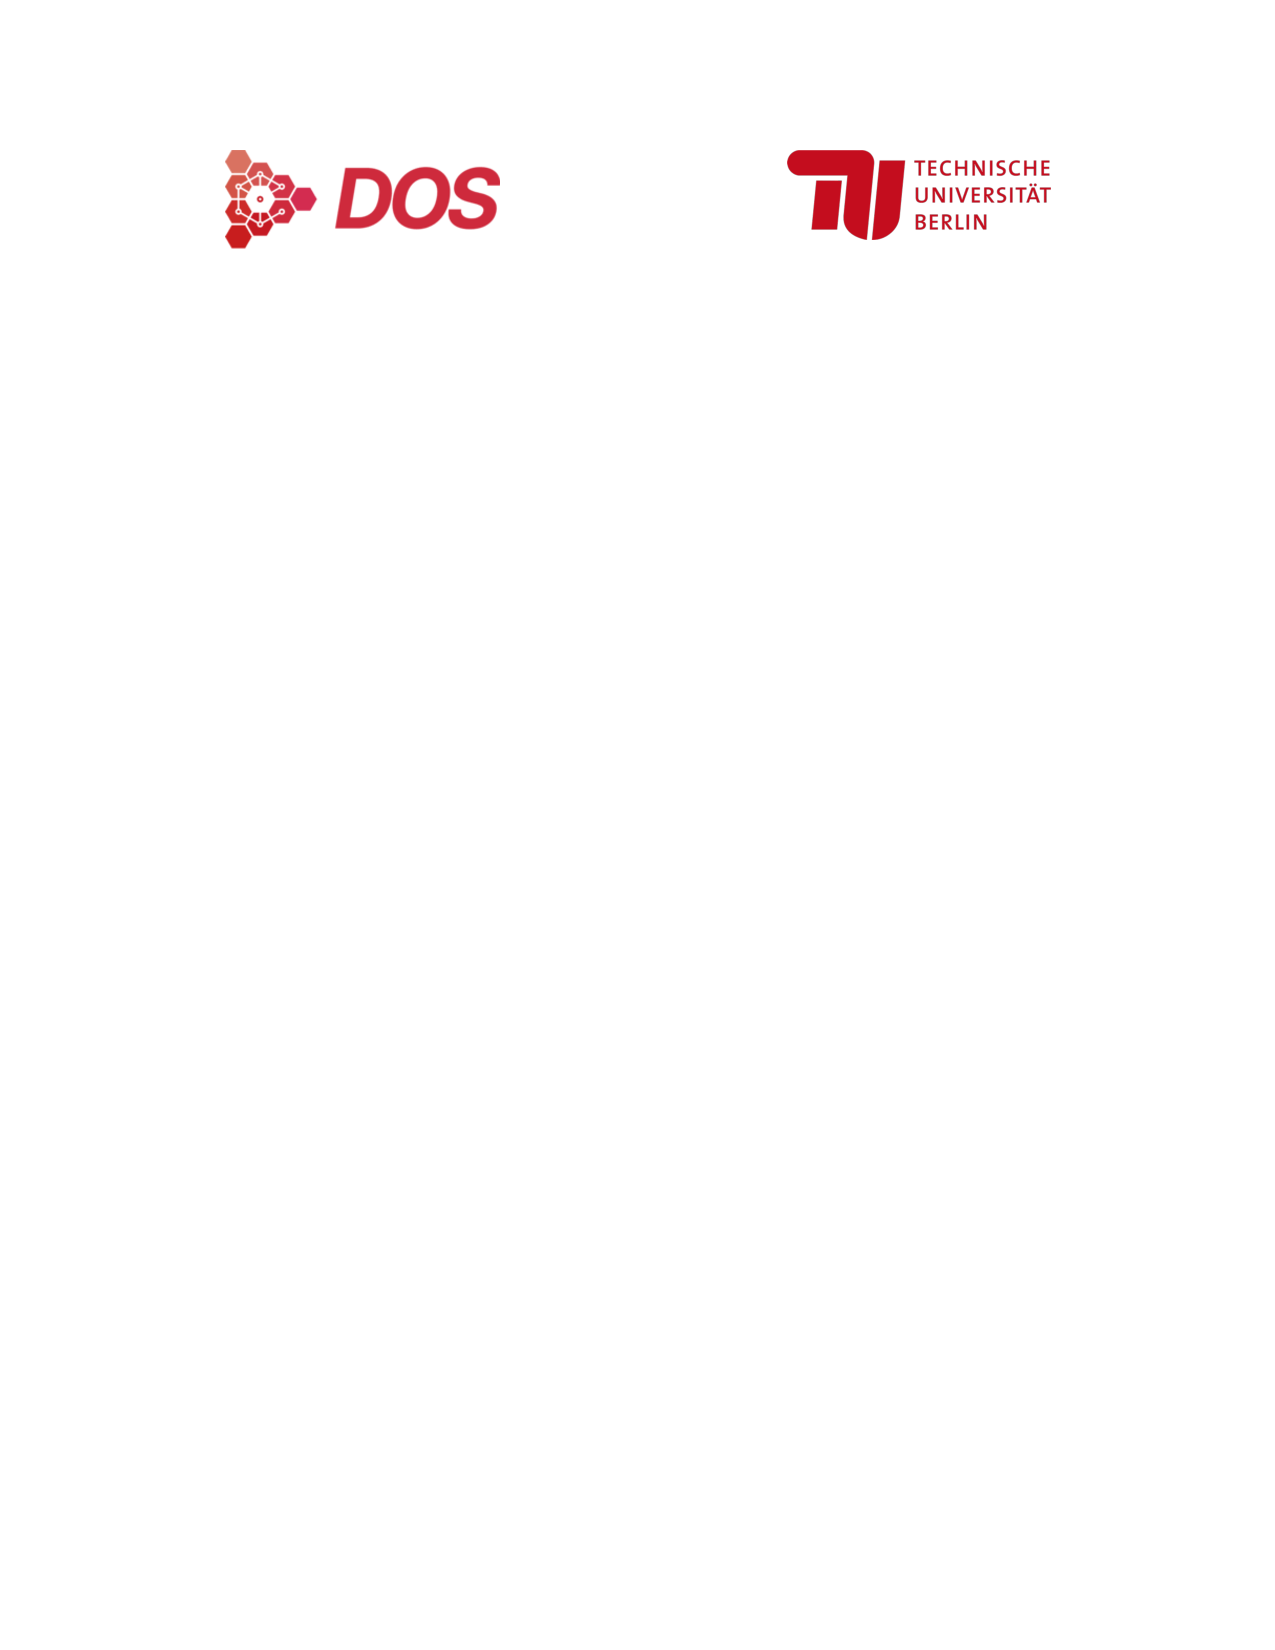
\includegraphics[width=\paperwidth]{title.pdf}%
            \vfill
        }
    }
}

\vfill
\vspace*{5cm}

{\huge\textbf{\projectTitle}\par}
\vspace*{0.5cm}
\textbf{\thesisType}      \\
\vspace*{2cm}
\textbf{Author}               \\
\authors              \\
\matrikel                     \\
\authorEmail                  \\
\vspace*{1cm}
\textbf{Advisor}              \\
\supervisor                   \\
\vspace*{1cm}
\textbf{Examiners}            \\
\examinera                    \\
\examinerb

\vfill

\textbf{Technische Universit\"at Berlin, \projectYear} \\
\small{\facultyName \\
    \departmentName}
\vspace{1cm}
}

\thispagestyle{empty}
\clearpage

\vspace*{\fill}
\begin{centering}
    {\huge\textbf{\projectTitle}\par}
    \vspace{1cm}
    \large{\thesisType}\\
    \vspace{1cm}
    Submitted by:\\
    \authors\\
    \matrikel                     \\
    \authorEmail                  \\
    \vspace{1cm}
    Technische Universit\"at Berlin\\
    \facultyName \\
    \departmentName \\
    \vspace{1cm}
    \projectYear\\

\end{centering}

\vspace*{\fill}
\thispagestyle{empty}
\clearpage

\vspace*{\fill}
{
    % briefly set the footnote to symbols for this disclaimer
    \renewcommand*{\thefootnote}{\fnsymbol{footnote}}
    \noindent
    \begin{otherlanguage}
        {ngerman}
        Hiermit versichere ich, dass ich die vorliegende Arbeit eigenständig ohne Hilfe Dritter und ausschließlich unter Verwendung der aufgeführten Quellen und Hilfsmittel angefertigt habe.
        Alle Stellen die den benutzten Quellen und Hilfsmitteln unverändert oder sinngemäß entnommen sind, habe ich als solche kenntlich gemacht.

        Sofern generische KI-Tools verwendet wurden, habe ich Produktnamen, Hersteller, die jeweils verwendete Softwareversion und die jeweiligen Einsatzzwecke (z.~B.~sprachliche Überprüfung und Verbesserung der Texte, systematische Recherche) benannt.
        Ich verantworte die Auswahl, die Übernahme und sämtliche Ergebnisse des von mir verwendeten KI-generierten Outputs vollumfänglich selbst.

        Die Satzung zur Sicherung guter wissenschaftlicher Praxis an der TU Berlin vom 8. März 2017\footnote{\url{https://www.static.tu.berlin/fileadmin/www/10000060/FSC/Promotion___Habilitation/Dokumente/Grundsaetze_gute_wissenschaftliche_Praxis_2017.pdf}} habe ich zur Kenntnis genommen.

        Ich erkläre weiterhin, dass ich die Arbeit in gleicher oder ähnlicher Form noch keiner anderen Prüfungsbehörde vorgelegt habe.
        \vskip 2cm
        \begin{tabular}{@{}p{.5in}p{4in}@{}}
             & \hrulefill                              \\
             & (Unterschrift) \authors, Berlin, \today \\
        \end{tabular}

    \end{otherlanguage}
    % reset footnote styling for the rest of the thesis
    \renewcommand*{\thefootnote}{\arabic{footnote}}
    \setcounter{footnote}{0}
}

\vspace*{\fill}
\thispagestyle{empty}
\clearpage

\clearpage
\pagestyle{plain}

\newpage
\section*{Abstract}

FaaS is a cutting-edge new service model that has developed with the current advancement of cloud computing.
It allows software developers to deploy their applications quickly and with needed flexibility and scalability, while keeping infrastructure maintenance requirements very low.
These benefits are very desirable in edge computing, where ever-changing technologies and requirements need to be implemented rapidly and the fluctuation and heterogeneity of service consumers is a considerable factor.
However, edge nodes can often provide only a fraction of the performance of cloud computing infrastructure, which makes running traditional FaaS platforms infeasible.
In this thesis, we present a new approach to FaaS that is designed from the ground up with edge computing and IoT requirements in mind.
To keep it as lightweight as possible, we use CoAP for communication and Docker to allow for isolation between tenants while re-using containers to achieve the best performance.
We also present a proof-of-concept implementation of our design, which we have benchmarked using a custom benchmarking tool, and we compare our results with benchmarks of Lean OpenWhisk, another FaaS platform for the edge.
We find that our platform can outperform Lean OpenWhisk in terms of latency and throughput in all tests but that Lean OpenWhisk has higher success rates for a low number of simultaneous clients.

% GERMAN
\clearpage
\begin{otherlanguage}{ngerman}
  \section*{Kurzfassung}
  FaaS ist ein innovatives neues Servicemodell, das sich mit dem aktuellen Vormarsch des Cloud Computing entwickelt hat.
  Softwareentwicklende können ihre Anwendungen schneller und mit der erforderlichen Flexibilität und Skalierbarkeit bereitstellen und gleichzeitig den Wartungsaufwand für die Infrastruktur sehr gering halten.
  Diese Vorteile sind im Edge-Computing sehr wünschenswert, da sich ständig ändernde Technologien und Anforderungen schnell umgesetzt werden müssen und die Fluktuation und Heterogenität der Service-Consumer ein wichtiger Faktor ist.
  Edge-Nodes können jedoch häufig nur einen Bruchteil der Leistung von Cloud-Computing-Infrastruktur bereitstellen, was die Ausführung herkömmlicher FaaS-Plattformen unmöglich macht.
  In dieser Arbeit stellen wir einen neuen Ansatz für FaaS eine Platform vor, die von Grund auf unter Berücksichtigung von Edge-Computing- und IoT-Anforderungen entwickelt wurde.
  Um den Overhead so gering wie möglich zu halten, nutzen wir CoAP als Messaging-Protokoll und Docker, um Applikationen voneinander zu isolieren, während Container wiederverwendet werden, um die bestmögliche Leistung zu erzielen.
  Wir präsentieren auch eine Proof-of-Concept-Implementierung unseres Designs, die wir mit einem eigenen Benchmarking-Tool getestet haben, und vergleichen unsere Ergebnisse mit Benchmarks von Lean OpenWhisk, einer weiteren FaaS-Plattform für die Edge.
  Wir stellen fest, dass unsere Plattform Lean OpenWhisk in Bezug auf Latenz und Durchsatz in allen Tests übertreffen kann, Lean OpenWhisk jedoch höhere Erfolgsraten bei einer geringen Anzahl gleichzeitiger Clients aufweist.
\end{otherlanguage}

\clearpage

\tableofcontents
\clearpage

\section{Introduction}
\label{cha:introduction}

% Data Center Graph, then bridge gap to HPC and Scientific Workflows,Mention that a lot was done in HPC Co-Scheduling and also with the co-scheduling paradigm in cloud computing or interfernce with latency-sensitive jobs but not very much with co-location strategies themselves. Make a nice example of such a problem and how it looks like and why it can be beneficial.
\subsection{Problem Motivation \& Description}
\label{subse:problem_motivation_description}
% Section 1: Start with my graph and the initial problem
The rapid growth in data center power consumption has emerged as a pressing societal issue. As of March 2024, global statistics report more than 9,000 operational data centers worldwide, with this number continuing to rise steadily. Consequently, total annual energy consumption across data centers has been roughly doubling every four years with some now reaching capacities of up to 500 MW, comparable to the electricity demand of a city of one million residents. With the rapid growth in data volumes and processing requirements over the last two decades, workflow applications have grown in complexity, while computing infrastructures have advanced in processing capacity and workload management capabilities \cite{Coleman_2021}.
High-performance computing (HPC) refers to the pursuit of maximizing computational capabilities through advanced technologies, methodologies, and applications, enabling the solution of complex scientific and societal problems [citation]. HPC data centers consist of large numbers of interconnected compute and storage nodes, often numbering in the thousands, and rely on job schedulers to allocate resources, manage queues, and monitor execution. While these infrastructures provide the backbone for highly demanding applications, their intensive power draw does not only arise from computation but also from networking, cooling, and auxiliary equipment and makes them major consumers of electricity and significant contributors to climate change \cite{Silva_2024}.

% Figure
\begin{figure}[H]
    \centering
    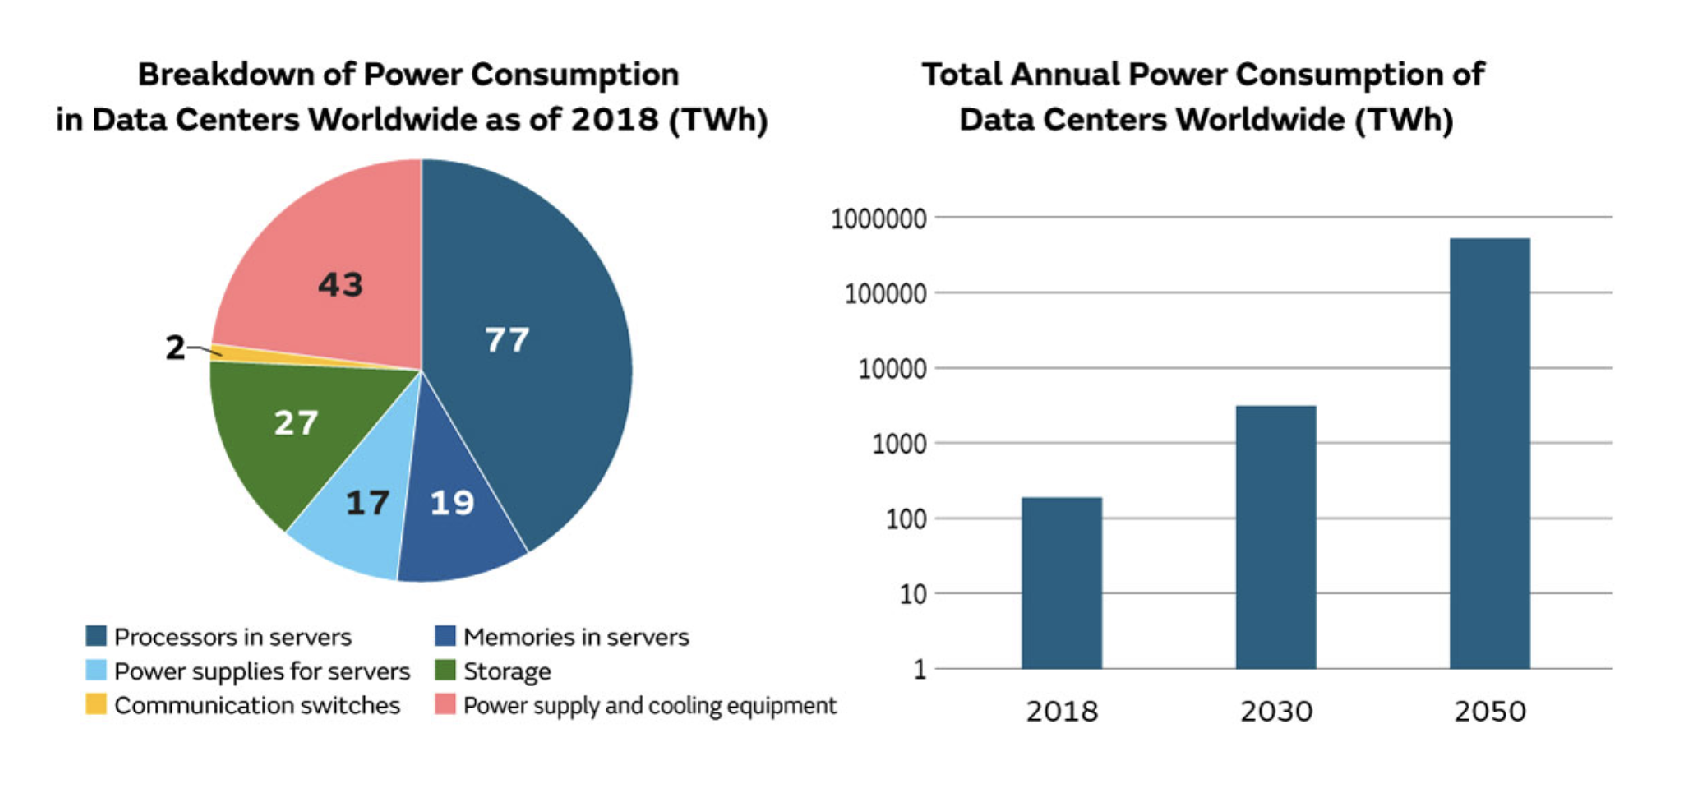
\includegraphics[scale=0.5]{fig/01/01-motivation.pdf}
    \small
    \caption{Breakdown of power consumption in data centers}
    \label{fig:01-motivation}
    \tiny
    Breakdown of power consumption in data centers and future outlook for power consumption.
\end{figure}

% Section 2: Move on to HPC and Workflows
A key driver of this trend is the exponential growth in data collection, storage, and processing across scientific disciplines. Scientific Workflow Management Systems (SWMSs) have become essential tools for managing this complexity, enabling researchers to exploit computing clusters for large-scale data analysis in domains such as remote sensing, astronomy, and bioinformatics. However, workflows executed through SWMSs are often long-running, resource-intensive, and computationally demanding, which translates into high energy consumption and substantial greenhouse gas emissions. Nevertheless, practitioners face challenges in assessing which approaches for mitigation are most applicable, effective with concerns to multiple objectives \cite{thamsen2025energyawareworkflowexecutionoverview}.
One central objective that this work focuses on is grounded in the challenge that tasks within data-driven workflows often appear in multiple instances and may vary substantially depending on input data, parameters, or execution environments their patterns in resource demand, energy consumption, and carbon emissions fluctuate during runtime rather than remaining constant.
This work primarily focuses on an aspect of workflow research that has received limited attention: modeling and managing the co-location of parallel tasks in containers and virtual machines.
To address this challenge, we apply continuous monitoring to enable fine-grained, time-dependent task models that accurately capture resource usage patterns. The central objective of this work is to leverage knowledge of task behavior to enhance the co-location process—the intermediate stage between task-to-machine mapping and scheduling—where decisions are made about which tasks should share compute resources to balance performance and energy efficiency.
While related concepts have been explored in the context of co-scheduling at the operating system level or in cloud environments where batch jobs run alongside latency-critical services, the online co-location problem addressed here differs. In our setting, decisions about which tasks to execute together on the same virtual machine must be made dynamically at each scheduling interval, requiring continuous adaptation to the current workflow state and resource conditions. The importance of such decisions can be illustrated through an example by \cite{inproceedings}. Consider two compute-bound programs (A1, A2) and two memory-bound programs (B1, B2) to be co-scheduled across two nodes. If both compute-bound tasks share one node while both memory-bound tasks share the other, the memory-intensive programs will heavily compete for bandwidth, causing severe slowdowns and doubling their execution time. In contrast, pairing each compute-bound task with a memory-bound one allows both to utilize different resources efficiently, resulting in no slowdown at all. This demonstrates two fundamental principles of co-location: tasks that heavily use the same resource should not be co-located, and complementary resource usage—such as pairing CPU-intensive and memory-intensive workloads—can maximize system performance.
Furthermore, previous studies have shown that effective co-scheduling of this kind can significantly enhance both energy efficiency and system throughput in high-performance computing environments. In the best cases, runtime can be reduced by up to 28\% and total energy consumption by approximately 12\% compared to isolated, dedicated execution. However, the extent of improvement depends strongly on the diversity and ratio of jobs in the scheduling queue \cite{7349920}. To address this, we propose a hierarchical clustering approach that groups tasks by dissimilarity to encourage complementary co-location. This mechanism is integrated into a workflow simulation framework, where several scheduling algorithms are implemented to demonstrate how informed, runtime co-location decisions can enhance task mapping and overall workflow efficiency.

% TODO: make cursive
These challenges motivate the central goal of this work: modelling the complementary co-location of scientific workflow tasks using fine-grained, time-dependent resource usage profiles and embedding it into workflow execution for energy and performance aware decision making during runtime.

\subsection{Research Question \& Core Contributions}
\label{subse:research_question_core_contributions}

The central questions this thesis seeks to address are:

\begin{enumerate}[label=\textbf{RQ}\arabic*]
    \item How can fine-grained, time-dependent models of workflow tasks be developed to capture fluctuating patterns of computational resource usage and energy consumption during execution?
    \item How can the co-location of workflow tasks be modeled so that their interference is minimized and the resulting shared usage of resources leads to lower overall energy consumption and carbon emissions while performance is maintained?
    \item How can co-location models and time-dependent task characterizations be integrated into resource management systems and workflow scheduling frameworks to enable adaptive, energy-aware execution at scale?
\end{enumerate}

% TODO: Add footnote for nf-core repo
The resulting core contributions of this thesis are:
\begin{itemize}
    \item The implementation of a monitoring client, capable of serving the relevant monitoring layers for scientific workflow execution which collects fine-grained, time-dependent resource usage data for workflow tasks during execution that was used for low-level data collection on 9 nf-core pipelines.
    \item The design and further development of a novel online task co-location approach that utilizes time series data to compute for any given set of tasks clusters with complementary resource usage patterns.
    \item The development of a simulator that integrates the proposed co-location approach into the workflow execution phase.
    \item The conceptual implementation of a scheduler, able to predict the performance and energy consumption of co-located tasks using two machine learning models.
    \item The evaluation of the co-location approach in simulation using 9 nf-core workflows, demonstrating its effectiveness in reducing energy consumption while maintaining performance.
\end{itemize}
\subsection{Structure of the Thesis}
\label{subse:structure_of_the_thesis}
The remainder of this thesis is structured as follows: Chapter \ref{cha:background} presents the fundamentals of this work, covering performance monitoring, scientific workflow systems, the co-location problem, cluster resource management and machine learning. Chapter \ref{cha:relatedwork} introduces related work within the domain of optimizing Scientifc Workflow execution and objectives in line with these of this work. Furthermore, Chapter \ref{cha:approach} depicts the approach to the problem in both a theoretical and practical manner and ultimately defines the realization of the approach. The corresponding implementation is elaborated in Chapter \ref{cha:implementation}. Moreover, Chapter \ref{cha:evaluation} evaluates the steps conducted to achieve the implementation of the overall approach using both empirical data and a simulation environment. Chapter \ref{cha:discussion} interprets the key findings and discusses some limitations of this work. Finally, Chapter 8 concludes this thesis and gives an outlook on the impact of this work for the future.

\clearpage
\section{Background}
\label{cha:background}

This chapter provides the necessary background for the thesis. Section 2.1 introduces the domain of High-Performance Computing (HPC), with a focus on modern computational hardware (2.1.1) and virtualization technologies (2.1.2). Section 2.2 then discusses scientific workflows as a representative HPC application, beginning with a definition of scientific workflows (2.2.1), followed by their management systems (2.2.2), and concluding with workflow tasks as their smallest management unit (2.2.3). Section 2.3 introduces the domain of energy-aware computing, while Section 2.4 addresses workflow monitoring, including monitoring targets (2.4.1), resource monitoring (2.4.2), energy monitoring (2.4.3), and task characterization using monitoring data (2.4.4). Section 2.5 presents the co-location problem, which constitutes the core of this thesis. It motivates the problem through resource contention (2.5.1), discusses its relationship to workflow scheduling and task mapping (2.5.2), and provides a general overview with the guiding boundaries that shape the definition of workflow task co-location used throughout this work. Section 2.6 introduces the role of machine learning in scientific workflow processing, focusing on its application in resource management (2.6.1) and the theoretical background of the models applied in this thesis. This includes Kernel Canonical Correlation Analysis (KCCA) (2.6.2.1), Random Forest Regression (2.6.2.2), Linear Regression (2.6.2.3), and Agglomerative Clustering for task clustering (2.6.2.4). Finally, Section 2.7 outlines the evaluation methodology, with an emphasis on simulation approaches and a description of the WRENCH framework for simulating distributed computing environments (2.7.1).

\subsection{High Performance Computing}
\label{sec:background_hpc}
% TODO: Include citation HPC book, Chapter 1.1
High-Performance Computing (HPC) encompasses a collection of interrelated disciplines that together aim to maximize computational capability at the limits of current technology, methodology, and application. At its core, HPC relies on specialized electronic digital machines, commonly referred to as supercomputers, to execute a wide variety of computational problems or workloads at the highest possible speed. The process of running such workloads on supercomputers is often called supercomputing and is synonymous with HPC. The fundamental purpose of HPC is to address questions that cannot be adequately solved through theory, empiricism, or conventional commercial computing systems. The scope of problems tackled by supercomputers extends beyond traditional scientific and engineering applications to include challenges in socioeconomics, the natural sciences, large-scale data management, and machine learning. An HPC application refers both to the problem being solved and to the body of code, or ordered instructions, that define its computational solution.

What distinguishes HPC systems from conventional computers is their organization, interconnectivity, and scale. Here, scale refers to the degree of both physical and logical parallelism: the replication of essential physical components such as processors and memory banks, and the partitioning of tasks into units that can be executed simultaneously. While parallelism exists in consumer devices like laptops with multicore processors, HPC systems exploit it on a vastly larger scale, structured across multiple hierarchical levels. Their supporting software is designed to orchestrate and manage operations at this level of complexity, ensuring efficient execution across thousands of interconnected components.

\subsubsubsection{Modern HPC Hardware}
\label{sec:background_hpc_hardware}
% Include graphic inspired from Chapter 1.1, page 7 of HPC book.
High performance computer architecture determines how very fast computers are formed and function. High performance computing (HPC) architecture is not specifically about the lowest-level technologies and circuit design, but is heavily influenced by them and how they can be most effectively employed in supercomputers. HPC architecture is the organization and functionality of its constituent components and the logical instruction set architecture (ISA) it presents to computer programs that run on supercomputers. HPC architecture exploits its enabling technologies to minimize time to solution, maximize throughput of operation, and serve the class of computations associated with large, usually numeric-intensive, applications. In recent years supercomputers have been applied to data-intensive problems as well, popularly referred to as “big data” or “graph analytics”. For either class of high-end applications, HPC architecture is created to overcome the principal sources of performance degradation, including starvation, latency, overheads, and delays due to contention. It must facilitate reliability and minimize energy consumption within the scope of performance and data requirements. Cost is also a factor, affecting market size and ultimate value to domain scientists and other user communities. Finally, architecture shares in combination with the many other layers of the total HPC system the need to make application programming by end users as easy as possible.

HPC system performance depends on the speed of its components, with processor clock rate being a key factor. A major challenge arises from mismatches in cycle times across technologies, such as fast processor cores versus much slower DRAM. To bridge this gap, modern architectures use memory hierarchies that combine high-capacity DRAM with faster SRAM caches. Performance is also shaped by communication speed, measured in bandwidth and latency, which vary with technology and distance. Ultimately, HPC architecture seeks to balance computation, memory, and communication speeds while optimizing cost, power, and usability to maximize application performance.
Efficiency in HPC refers to how effectively system components are utilized when executing a workload. A common metric is floating-point efficiency, defined as the ratio of sustained floating-point performance to the theoretical peak, both measured in FLOPs. While once meaningful in an era when floating-point operations were costly, this measure has become less representative as data movement and memory access now dominate in terms of time, energy, and die space. Nevertheless, FLOP-based efficiency remains the most widely reported measure.

Power consumption is a critical factor in HPC, as processors, memory, interconnects, and I/O devices all require electricity, and the resulting heat must be removed to avoid failure. Processor sockets alone may consume 80–200 W, and cooling adds significant overhead, sometimes exceeding 20\% of total power use. Air cooling suffices for smaller systems, but high-density, high-performance systems increasingly rely on liquid cooling to achieve higher packing density and performance. Modern processors further support power management through dynamic voltage and frequency scaling, variable core activation, and thermal monitoring. These mechanisms enable a balance between power consumption and performance, guided by software that can set or adjust configurations at runtime based on workload demands.

The multiprocessor class of parallel computer represents the dominant architecture in contemporary supercomputing. Broadly defined, it consists of multiple independent processors, each with its own instruction control, interconnected through a communication network and coordinated to execute a single workload. Three main configurations of multiprocessor systems exist: symmetric multiprocessors (SMPs), massively parallel processors (MPPs), and commodity clusters. The distinction lies in memory organization. SMPs use a shared memory model accessible by all processors, MPPs assign private memory to each processor, and cluster-based designs combine both approaches by grouping processors into nodes that share memory locally while maintaining separation across nodes. Modern multicore systems often follow this hybrid structure, balancing performance, scalability, and complexity.
% TODO: Maybe include graphic that shows overview

A shared-memory multiprocessor consists of multiple processors with direct hardware access to a common main memory. This architecture allows any processor to read or write data produced by another, requiring an interconnection network that ensures cache coherence across all processors. Cache coherence guarantees correctness by keeping local caches consistent, often implemented through protocols such as MESI, where writes are detected and other caches are updated or invalidated accordingly.

Shared-memory multiprocessors are commonly divided into two categories based on memory access times. In symmetric multiprocessors (SMPs), all processors can access any memory block in equal time, known as uniform memory access (UMA). While contention for memory banks can still cause delays, the system provides equal opportunity to all processors. SMPs are widely used in enterprise servers, workstations, and multicore laptops, and often serve as nodes within larger parallel systems.

Nonuniform memory access (NUMA) architectures extend shared-memory designs by allowing all processors to access the full memory space but with different access times depending on locality. NUMA leverages fast local memory channels alongside slower global interconnects, enabling greater scalability than SMPs. However, this places additional responsibility on software developers to optimize data placement in order to achieve high performance. NUMA systems emerged in the late 20th century and remain a key design for scaling shared-memory multiprocessors.

% TODO: Add NUMA graphic
% TODO: Add AMD stuff

\subsubsection{Virtualization in HPC}
\label{sec:background_hpc_virtualization}
% TODO: Cite paper: Survey on Virtualization of HPC, M. Shao IEEE
With the growing demand for High-Performance Computing (HPC), hardware resources have continued to expand in scale and complexity, with increasingly intricate interconnections between system components. A central challenge lies in maximizing both performance and resource utilization. Virtualization technologies offer a means to improve resource utilization in HPC environments, but often at the cost of performance overhead. Multi-user usage scenarios, combined with the stringent performance requirements of HPC workloads, place high demands on virtualization approaches. Furthermore, the highly customized nature of HPC systems complicates the integration of virtualization solutions. This work examines operating system-level and application-level virtualization within HPC, outlines the current limitations, and discusses potential directions for future developments.

Virtualization at the operating system level has been widely explored through technologies such as VMware, Xen, LXC, and KVM, each offering different trade-offs between usability, security, and performance. VMware, one of the earliest and most established solutions, allows multiple operating systems to run simultaneously on a single host, offering strong isolation, security, and ease of configuration. However, the performance overhead introduced by full virtual machines is too high for HPC workloads, which demand near-native computational speed. Xen, developed as an open-source virtual machine monitor, improved performance compared to VMware but required operating system modifications, making it less developer-friendly and leading to reduced long-term adoption. More recent solutions such as LXC and KVM integrate virtualization more closely with the Linux kernel, reducing overhead compared to traditional VMs. While these operating system–level containers are lighter than VMware or Xen, they still introduce performance penalties, with KVM in particular showing unacceptable overhead for CPU-intensive HPC applications. Moreover, KVM requires hardware-level virtualization support, limiting its applicability.

In multi-tenant HPC environments, the dynamic sharing of hardware resources introduces complex power–performance relationships, as concurrently executed tasks exhibit varying levels of power consumption across different resources. Users increasingly expect the flexibility of cloud-like environments, where execution conditions resemble their native setups without significant performance loss. Container-based HPC environments address this demand by isolating groups of processes into separate applications that run densely on available hardware threads. \cite{Kuity_2023}.

Virtualization enables the provisioning of resources to multiple users on the same physical machine with the goal of maximizing utilization. Depending on the abstraction layer, different virtualization technologies provide distinct benefits. Containers, which virtualize at the operating system level, offer lightweight isolation and have become widely adopted for deploying microservices. They effectively bridge the gap between development and production by supporting continuous integration and deployment pipelines.
Containers leverage the host operating system kernel and typically incur far less management and runtime overhead compared to virtual machines. Prior studies have shown that container performance often approaches native execution, particularly for CPU- and memory-intensive workloads, whereas VMs tend to suffer greater degradation for memory, disk, and network-intensive applications. In comparative analyses, Docker containers have demonstrated near-native efficiency for CPU and memory tasks but exhibit performance bottlenecks in certain networking and storage configurations. Research has also highlighted scalability challenges, including increased startup times as the number of containers grows, as well as interference effects when multiple containers share disk- or network-intensive workloads on the same host. These findings underline the fact that performance in containerized environments is strongly dependent on workload characteristics and resource contention patterns. Despite advances such as workload-aware brokering systems aimed at improving energy efficiency and utilization, limited attention has been paid to how workload nature and interference influence consolidation decisions \cite{8397647}.

% TODO: Cite paper: Survey on Virtualization of HPC, M. Shao IEEE
Application-level virtualization operates above the kernel layer, sharing both the kernel and underlying hardware. This approach is most prominently represented by containers, with Docker introducing a transformative model of packaging and deployment. By encapsulating application dependencies into images and leveraging ecosystems such as Docker Hub, Docker enables rapid and portable application deployment. However, in HPC environments, Docker raises serious concerns. Security risks emerge from its daemon-based execution model, which runs with root privileges, and its resource allocation mechanism conflicts with HPC scheduling managers like Slurm, PBS, or SGE. These schedulers typically rely on cgroups to enforce job-level resource limits, but such constraints are ineffective when bypassed by Docker’s daemon. Furthermore, Docker lacks robust support for MPI and multi-node collaboration, making it unsuitable for large-scale HPC workloads.

% TODO: Cite paper: Survey on Virtualization of HPC, M. Shao IEEE
To address these issues, container solutions such as Singularity and Shifter were developed specifically with HPC requirements in mind. Singularity allows users to build and test applications in local environments and then deploy them seamlessly on HPC systems. Unlike Docker, it does not rely on a persistent daemon, thus resolving security and resource management concerns. Singularity also supports multiple container image formats, including compatibility with Docker images, and integrates efficiently with HPC resource managers. Its design ensures that containers incur minimal overhead, as virtualization occurs only at the application level with a shared kernel, making it particularly well-suited for HPC contexts where performance efficiency is critical.

% TODO: Containerization graphic
% TODO: Virtual Machine graphic

\subsection{Scientific Workflows}
\label{sec:background_workflows}

% TODO: Include more stuff from 
% \cite{Scientific worflows: past, present and future}
\subsubsection{Scientific Workflow Management Systems}
\label{sec:background_workflows_swms}
Scientific Workflow Management Systems (SWMSs) enable the composition of complex workflow applications by connecting individual data processing tasks. These tasks, often treated as black boxes, can represent arbitrary programs whose internal logic is abstracted away from the workflow system. The resulting workflows are typically modeled as directed acyclic graphs (DAGs), where channels define the dependencies between tasks: the output of one task serves as the input for one or more downstream tasks. This abstraction allows users to design scalable, reproducible workflows while managing execution complexity across diverse computational environments \cite{thamsen2025energyawareworkflowexecutionoverview}.

Scientific Workflow Management Systems (SWMSs) provide a simplified interface for specifying input and output data, enabling domain scientists to integrate and reuse existing scripts and applications without rewriting code or engaging with complex big data APIs. This abstraction lowers the entry barrier for developing and executing large-scale workflows. In parallel, cloud computing has become an increasingly popular execution environment, complementing or replacing traditional HPC clusters. Clouds offer advantages such as elastic scalability, flexible pay-as-you-go pricing models, and access to a wide range of heterogeneous hardware resources, making them attractive for diverse workflow workloads \cite{Bader_2022}.

% TODO: Add graphic of SWMS architecture in general

\subsubsection{Examples of Scientific Workflows}
\label{sec:background_workflows_examples}
% TODO: Add graphic of pipeline 
Scientific workflows are compositions of sequential and con- current data processing tasks, whose order is determined by data interdependencies [4]. A task is the basic data process- ing component of a scientific workflow, consuming data from input files or previous tasks and producing data for follow- up tasks or output files (see Figure 1). A scientific workflow is usually specified in the form of a directed, acyclic graph (DAG), in which individual tasks are represented as nodes. Scientific workflows exist at different levels of abstraction: abstract, concrete, and physical. An abstract workflow mod- els data flow as a concatenation of conceptual processing steps. Assigning actual methods to abstract tasks results in a concrete workflow. If this mapping is performed auto- matically, it is called workflow planning [5]. To execute a concrete workflow, input data and processing tasks have to be assigned to physical compute resources. In the context of scientific workflows, this assignment is called scheduling and results in a physical and executable workflow [6]. Low-level batch scripts are a typical example of physical workflows \cite{Bux2013}.

% TODO: Add section about HPC and Scientific Workflows with reference to earlier section
\subsubsection{Scientific Workflow Tasks}
\label{sec:background_workflows_examples}
Workflow applications are typically executed per input, or per set of related inputs, enabling coarse-grained data parallelism at the application level. Multiple tasks can run concurrently if independent inputs are processed by the same workflow, and parallelism also arises within a single input when workflow graphs fork, allowing downstream tasks to execute simultaneously. Conversely, many workflows begin with parallel execution of different tasks whose outputs are later joined, synchronizing multiple workflow paths.

Due to their complexity and scale, workflows often consist of large numbers of tasks with multiple parallel paths and are executed on clusters—collections of interconnected compute nodes managed as a single system. Scientific Workflow Management Systems (SWMSs) submit ready-to-run tasks to cluster resource managers such as Slurm or Kubernetes, which allocate resources according to user-defined requirements like CPU cores and memory. Task communication is typically implemented via persistent cluster storage systems (e.g., Ceph, HDFS, or NFS), where intermediate data is written and read between tasks. This approach ensures flexible scheduling, fault tolerance through restartable intermediate states, and simplified execution management.

While SWMSs usually treat tasks as black boxes, opening these tasks for optimization can significantly improve performance. In particular, adapting code to the available hardware, such as optimizing for specific CPUs or accelerators, can reduce runtime. Since certain code segments disproportionately affect overall task execution time, focusing on these hotspots offers an effective strategy for workflow-level performance improvement \cite{thamsen2025energyawareworkflowexecutionoverview}.

% TODO: Add graphic of task 
% TODO: Mention task disclaimer for writing ease


\subsection{Energy-Aware Computing}
\label{sec:background_energyawarecomputing}
% TODO: Include more examples of the relevancy of energy-aware computing
\cite{thamsen2025energyawareworkflowexecutionoverview}
Power consumption in computing systems can broadly be divided into static and dynamic components. Static power is drawn even when components are idle, often reaching up to half of peak power, while dynamic power depends on utilization and increases with workload. This inefficiency has motivated the concept of energy-proportional computing, in which energy use per operation scales directly with utilization. Hardware trends and techniques such as Dynamic Voltage and Frequency Scaling (DVFS) have improved proportionality, while workload consolidation further increases efficiency by concentrating tasks on fewer resources.

Beyond compute, data centers also consume energy for cooling, lighting, and auxiliary operations. This is measured by Power Usage Effectiveness (PUE), which expresses the ratio between total data center energy use and the share consumed by IT equipment. While leading hyperscale centers achieve PUE values close to 1.1, the global average remains higher, and the metric has known limitations, including sensitivity to workload characteristics and the inability to capture whole-system trade-offs.

The climate impact of energy use further depends on carbon intensity, i.e., the emissions associated with each unit of consumed electricity. This varies geographically and temporally with the mix of fossil, nuclear, and renewable generation sources. As such, carbon intensity can fluctuate substantially over hours and regions, meaning that both location and timing of computation influence emissions.

Breaking down component-level energy use, CPUs typically dominate server consumption, accounting for 40–66\% of total power, with significant static and dynamic contributions. Memory is the second largest consumer, drawing a smaller but relatively stable share, while storage devices show limited dynamic variation and modest overall consumption. Networking equipment consumes comparatively little, with low dynamic variation, though attributing its energy use to specific workloads is non-trivial.

A geoscience workflow (FORCE) was executed on a commodity cluster using 21 nodes for 315 minutes to process 304 GB of satellite images. The hardware setup led to an estimated operational energy use of 15.8 kWh, factoring in average data center overhead (PUE 1.61). Given Germany’s 2021 grid carbon intensity of 439 gCO₂e/kWh, this corresponds to about 6.95 kgCO₂e emissions per run, or 20.8 kgCO₂e for the three repetitions used to report median results—roughly equal to driving 53 miles in a gasoline car. Beyond operational emissions, the embodied carbon footprint of the hardware was considered. With an estimated 1200 kgCO₂e per node over its lifetime and 0.00599\% of lifetime usage during the experiment, the workflow’s share amounts to about 1.5 kgCO₂e per run, or 4.5 kgCO₂e for three executions. Thus, both operational and embodied emissions contribute to the total footprint of the workflow evaluation.

\subsection{Monitoring Scientific Workflows}
\label{sec:background_monitoring}

\subsubsection{Performance Monitoring}
\label{sec:background_monitoring_performance}
% TODO: Insert citation for HPC Book
Performance monitoring is a critical stage in application development, extending beyond functional correctness and validation of results. Even after thorough testing with diverse datasets and computational modes, hidden inefficiencies may remain that limit the application’s ability to fully exploit the underlying hardware. This is especially significant in parallel computing, where inefficiencies are amplified across many processor cores, leading not only to longer runtimes but also to higher computational costs, as users are often charged proportionally to aggregate machine time. Monitoring helps ensure that performance is not degraded by preventable factors, for example by checking whether computation times match processor capabilities or whether communication delays align with message sizes and network bandwidth. Instrumentation of code segments can provide such insights, though even basic measurements introduce latency and overhead that may distort results or even alter execution flow. To reduce this, statistical sampling is often employed, recording snapshots of program state at intervals rather than logging every event. Sampling periods can be tuned to balance accuracy against intrusiveness. Hardware-based approaches offer another alternative: modern CPUs provide dedicated performance counters for events such as instruction retirement, cache misses, or branches. These counters operate transparently, incurring virtually no overhead, though they are limited to a predefined set of measurable events. Together, these techniques form the basis of effective performance monitoring, allowing developers to identify and address bottlenecks without unduly interfering with execution.

\subsubsection{Monitoring Layers}
\label{sec:background_monitoring_layers}
While low-level tools can provide detailed insights into system resource usage, linking these measurements to higher-level abstractions such as workflow tasks remains challenging. In large-scale scientific workflows executed on distributed environments like clusters or clouds, tasks may be scheduled on arbitrary nodes and may even share resources with other tasks. As a result, locally observed traces of CPU, memory, or I/O usage cannot be directly attributed to specific tasks. To bridge this gap, resource usage profiles from compute nodes must be correlated with metadata such as workflow logs or job orchestrator information (e.g., container management data). Establishing this information chain enables the classification of observed behavior at the task level, highlighting inefficient or resource-intensive components of the workflow that offer the greatest potential for optimization.

Existing monitoring frameworks focus primarily on processes or systems and generally lack the ability to map resource usage back to workflow tasks, especially in multi-tenant or distributed environments. This limits the ability to isolate the contribution of individual tasks to overall resource consumption. Moreover, metrics natively provided by workflow management systems are often coarse-grained, capturing only summary statistics for task lifetimes. To obtain fine-grained insights into task-level behavior, additional instrumentation and mapping strategies are required to connect low-level monitoring data with workflow abstractions \cite{Witzke2024}.

% TODO: Insert adapted graphic of monitoring layers, inspired by Bader.
The proposed architectural blueprint for workflow monitoring is structured into four layers: the resource manager, the workflow, the machine, and the task layer. These layers represent logical distinctions within a scientific workflow execution environment, each focusing on a different monitoring subject and retrieving metrics from lower layers as needed. Unlike user-centric designs, this approach emphasizes system components rather than interaction flows. Higher layers provide increasingly abstract views, relying only on selected metrics from underlying layers while, in theory, being able to access all. For instance, at the resource manager level, systems such as Slurm, Kubernetes, or HTCondor only require aggregate metrics like task resource consumption or available machine resources, without depending on fine-grained traces such as syscalls. The workflow layer captures metrics tied to the workflow specification, while the machine layer delivers detailed reports of node-level resource usage. At the lowest level, the task layer focuses on fine-grained task execution metrics. Together, this hierarchy balances abstraction and granularity, ensuring that relevant monitoring information is exposed at the appropriate level to support both workflow execution and performance optimization \cite{Bader_2022}.

The monitoring architecture is structured into four interdependent layers that capture different levels of abstraction within a workflow execution environment. At the top, the resource manager layer supervises the cluster, orchestrates task assignments, and provides coarse-grained monitoring. It contributes aggregated information such as active workflows, running and queued tasks, node health status, and distributed file system states. To enable correct task placement, it draws on workflow-level identifiers and DAG structures, machine-level metrics like available cores or memory, and task-level resource usage and execution status. The workflow layer refines this view by capturing execution semantics, such as dependencies between tasks expressed as DAGs, workflow progress, runtime statistics, makespan, and error reports. The machine layer focuses on per-node monitoring, reporting both general metrics (e.g., CPU and memory utilization) and fine-grained hardware characteristics such as architecture, clock rates, disk partitions, and virtualization context. At the lowest level, the task layer provides the most detailed insights, including logs, execution times, time-series resource usage, and kernel-level traces such as system calls or I/O activity. These fine-grained metrics are essential for diagnosing failures and identifying performance bottlenecks. Together, the four layers form a hierarchical structure where higher layers abstract and summarize information from lower ones, enabling a comprehensive and scalable approach to workflow monitoring \cite{Bader_2022}.

Scientific workflow management systems (SWMSs) provide varying degrees of built-in monitoring support, which is often complemented by external tools. Pegasus integrates tightly with HTCondor as its resource manager and submits monitoring data directly into a relational database, enabling real-time querying and visualization with external tools such as ElasticSearch or Grafana. Nextflow, originally developed for bioinformatics workflows, has since expanded into other domains and produces monitoring reports once workflow executions are complete. Airflow, with its strong integration into Python, exports selected metrics to StatsD, from where they can be forwarded to systems such as Prometheus for monitoring. Snakemake, also Python-based, supports report generation after execution and offers live monitoring through its Panoptes service, which streams data to an external server accessible via API. Argo, designed natively for Kubernetes, provides a web-based interface where users can access reports and logs of previous executions alongside live monitoring features. Despite these capabilities, most resource managers do not natively handle workflow-level submissions. Consequently, SWMSs typically manage task dependencies and submit tasks sequentially as their requirements are satisfied, with notable exceptions such as HTCondor’s DAGMan meta-scheduler and Slurm’s built-in dependency mechanisms \cite{Bader_2022}.

\subsubsection{Resource Monitoring}
\label{sec:background_monitoring_resource}
% TODO: Insert citation for ebpf book
Monitoring scientific workflows requires tools that can capture and relate information across different components of a computing system, since no single perspective provides sufficient detail for effective optimization. Low-level system monitors can reveal CPU, memory, or I/O usage but lack awareness of which workflow tasks generate that load, while workflow management systems expose task-level metrics that are often too coarse to identify inefficiencies. Similarly, resource managers like Slurm or Kubernetes aggregate machine usage but obscure fine-grained behavior. To close these gaps, specialized tools must be employed at each system layer—resource manager, workflow, machine, and task—and their outputs correlated. This layered approach ensures that high-level abstractions such as workflows can be linked to detailed system traces, allowing bottlenecks to be identified, failures diagnosed, and task placements optimized with respect to both performance and energy consumption. Without combining tools across layers, monitoring remains fragmented, leaving critical inefficiencies hidden in complex, distributed execution environments. In the following, we briefly discuss tools and approaches for monitoring each of these layers in detail while section % reference to section approach for monitoring
will go into much more detail.

Building on the need for layered monitoring, it is essential to introduce some fundamental terms and techniques that describe how monitoring data is collected and analyzed across system components. Central among these is tracing, which captures fine-grained event-based records such as system calls, I/O operations, or network packets. Tracing provides detailed raw data, often with high volume, that can either be post-processed into summaries or analyzed on the fly using programmatic tracers such as those enabled by the Berkeley Packet Filter (BPF). BPF allows small programs to run directly in the kernel, making it possible to process events in real time and reduce the overhead of storing and analyzing massive trace logs. In contrast, sampling tools collect subsets of data at regular intervals to create coarse-grained performance profiles. While sampling introduces less overhead than tracing, it provides only partial insights and can miss important events. Together with fixed hardware or software counters, tracing and sampling form the backbone of observability—the practice of understanding system behavior through passive observation rather than active benchmarking. Observability thus provides the conceptual umbrella under which monitoring tools operate, ranging from low-level system probes to workflow-aware abstractions. 
The BPF ecosystem provides several user-friendly front ends for tracing, most notably BCC (BPF Compiler Collection) and bpftrace. BCC was the first higher-level framework, offering C-based kernel programming support alongside Python, Lua, and C++ interfaces, and it introduced the libbcc and libbpf libraries that remain central to BPF instrumentation. It also provides a large collection of ready-to-use tools for performance analysis and troubleshooting. bpftrace, in contrast, offers a concise, domain-specific language that makes it well suited for one-liners and short custom scripts, while BCC is better for complex programs and daemons. A lighter-weight option, ply, is also being developed for embedded Linux environments. These frameworks, maintained under the Linux Foundation’s IO Visor project, collectively form what is often referred to as the BPF tracing ecosystem.These distinctions are crucial, as they shape how different tools are applied at the task, machine, workflow, and resource manager layers, and they form the basis for the more concrete monitoring techniques discussed in the following sections.

% TODO: Insert overview graph with monitoring targets on OS-level

Building on this, monitoring CPU usage fundamentally relies on understanding how time is distributed across these execution modes and how the scheduler allocates processor resources among competing tasks. Metrics such as user time, system time, and idle time provide the basis for identifying imbalances, while additional indicators like context switches, interrupt handling, and run queue lengths reveal how efficiently the scheduler manages concurrency. Since background kernel activities and hardware interrupts can consume significant CPU cycles outside of explicit user processes, distinguishing their contribution is essential for accurate analysis. Together, these metrics allow researchers and practitioners to detect inefficiencies such as excessive kernel overhead, overloaded cores, or unfair task distribution—insights that are critical when analyzing the performance of scientific workflows running on shared or large-scale computing infrastructures. A practical strategy for CPU performance analysis begins with verifying that a workload is running and truly CPU-bound, which can be confirmed through utilization metrics and run queue latency. Once established, usage should be quantified across processes, modes, and CPUs to identify hotspots such as excessive system time or uneven load distribution. Additional steps include measuring time spent in interrupts, exploring hardware performance counters like instructions per cycle (IPC), and using specialized BPF tools for deeper insights into stalls, cache behavior, or kernel overhead. This structured approach helps progressively narrow down the root causes of performance issues.
In close relation to CPU monitoring, effective memory performance analysis requires tracking how memory behavior influences compute efficiency. Since CPUs frequently stall waiting for data, metrics such as page faults, cache misses, and swap activity can directly translate into wasted cycles. A systematic strategy begins with checking whether the out-of-memory (OOM) killer has been invoked, as this signals critical memory pressure. From there, swap usage and I/O activity should be examined, since heavy swapping almost always leads to severe slowdowns. System-wide free memory and cache usage provide a high-level view of available resources, while per-process metrics help identify applications with excessive resident set sizes (RSS). Monitoring page fault rates and correlating stack traces can reveal which tasks or files drive memory pressure, while tracing allocation calls such as brk() and mmap() offers a complementary perspective on memory growth. At the hardware level, performance counters measuring cache misses and memory accesses give insights into where CPUs are stalling on memory I/O. Together, these monitoring steps build a detailed picture of how memory usage interacts with CPU performance, helping to uncover bottlenecks and inefficiencies that limit overall throughput.

Following CPU and memory, file system monitoring should focus on workload behavior at the logical I/O layer and its interaction with caches and the underlying devices. Key signals include operation mix and rates (reads, writes, opens/closes, metadata ops such as rename/unlink), latency distributions for I/O (including tails), and the balance of synchronous versus asynchronous writes. Cache effectiveness is central: track page-cache hit ratios over time, read-ahead usefulness (sequential vs random access), volumes of dirty pages and write-back activity, and directory/inode cache hit/miss rates. Attribute I/O to files and processes to spot hot files and short-lived file churn, and examine I/O size distributions to detect pathologically small requests. Relate logical I/O to physical I/O to assess whether caching is working or the workload is spilling to disk; include error rates and filesystem-specific events (e.g., journaling) for completeness. Finally, watch capacity and fragmentation risk (very high fill levels), mount options that affect performance semantics (e.g., atime, sync modes), and any lock contention visible in the file system path. A compact table or time-series dashboard for these metrics is helpful for diagnosis and comparison across workloads [cite].

In storage subsystems, background monitoring should characterize I/O where it matters for delivered performance and capacity planning rather than enumerate specific tools. At minimum, track request latency as a distribution (including tails) and decompose it into time queued in the operating system versus service time at the device; sustained high queue time indicates saturation regardless of nominal utilization. Measure throughput and IOPS per device together with queue depth to relate load to response, and record I/O size histograms and access locality (sequential vs. random) to explain latency modes. Distinguish operation classes—reads vs. writes, synchronous vs. asynchronous, metadata, readahead, flush/discard—since policies and devices handle them differently and they can interfere (e.g., reads stalling behind large write bursts). Attribute I/O to processes/containers and, where applicable, to workflow tasks so that noisy neighbors and hot spots can be isolated. Track error and timeout rates at the device interface to separate performance issues from reliability faults. Contextual signals such as filesystem cache hit ratio (logical vs. physical I/O), write-back pressure, and device fill level complement block-layer metrics and help explain shifts in latency or throughput. Segment all measurements per device and scheduling policy, and analyze them over time to identify persistent contention, bimodal behavior, and regressions that warrant tuning, task remapping, or rescheduling.

Containers are a lightweight virtualization technology that isolate applications while sharing the same host operating system kernel. Their implementation in Linux builds on two core mechanisms: namespaces, which provide isolation by restricting the view of system resources such as processes, file systems, and networks; and control groups (cgroups), which regulate resource usage, including CPU, memory, and I/O. Container runtimes such as Docker or orchestration frameworks like Kubernetes configure and combine these mechanisms to provide isolated execution environments. Two versions of cgroups exist in the kernel. Version 1 is still widely used in production systems, while version 2 addresses several shortcomings, including inconsistent hierarchies and limited composability, and is expected to become the default for containerized workloads in the near future.

From a performance monitoring perspective, containers introduce challenges that extend beyond those encountered in traditional multi-application systems. First, cgroups may impose software limits on CPU, memory, or disk usage that can constrain workloads before physical hardware limits are reached. Detecting such throttling requires monitoring metrics that are not visible through standard process- or system-wide tools. Second, containers can suffer from resource contention in multi-tenant environments, where “noisy neighbors” consume disproportionate shares of the available resources, leading to unpredictable performance degradation for co-located containers. This is particularly critical in Kubernetes deployments, where hundreds of containers may share a host and rely on fair scheduling enforced by the kernel and the container runtime.

A further complication lies in attribution. The Linux kernel itself does not assign a global container identifier. Instead, containers are represented as a combination of namespaces and cgroups, which complicates mapping low-level kernel events back to the higher-level abstraction of a specific container. While some workarounds exist—such as deriving identifiers from PID or network namespaces, or from cgroup paths—this mapping is non-trivial and runtime-specific. Consequently, many traditional monitoring tools remain container-unaware, often reporting host-level metrics even when executed inside containers. This mismatch can obscure important performance characteristics, such as CPU scheduling delays or memory pressure within a specific container, and may hinder the diagnosis of resource bottlenecks.

To address these issues, container monitoring must operate at multiple levels of abstraction. Metrics must capture both coarse-grained resource usage across cgroups and fine-grained kernel events such as scheduling latencies, memory allocation faults, and block I/O delays. At the same time, the collected data needs to be attributed correctly to the corresponding container environment in order to identify interference, diagnose bottlenecks, and evaluate orchestration policies. These requirements have motivated the use of extended monitoring techniques such as Berkeley Packet Filter (BPF) tracing, which can instrument kernel paths at runtime and associate low-level events with container-related constructs such as namespaces and cgroups.

Hypervisors enable hardware virtualization by abstracting physical resources and presenting them as fully isolated virtual machines, each running its own kernel. Two common configurations exist: bare-metal hypervisors, such as Xen, which schedule guest virtual CPUs directly on physical processors, and host-based hypervisors, such as KVM, which rely on a host kernel for scheduling. Both models often involve additional I/O handling layers, for example QEMU, which introduce latency but can be optimized through techniques such as shared memory transports and paravirtualized device drivers. Over time, virtualization efficiency has improved significantly with processor extensions like Intel VT-x and AMD-V, paravirtualization interfaces for hypercalls, and device-level virtualization (e.g., SR-IOV). Modern platforms, such as AWS Nitro, minimize software overhead by offloading core hypervisor functionality to dedicated hardware components.

Monitoring hypervisors poses challenges similar to containers but with a different focus. Since each VM runs its own kernel, guest-level monitoring tools can operate normally, but they cannot always observe the virtualization overheads introduced by the hypervisor. Key concerns include the frequency and latency of hypercalls in paravirtualized environments, the impact of hypervisor callbacks on application scheduling, and the amount of stolen CPU time—periods when a guest’s vCPU is preempted by the hypervisor. From the host perspective, additional events such as VM exits provide insight into how often guests trigger traps to the hypervisor, for example on I/O instructions or privileged operations, and how long these exits last. Attribution is further complicated because exit reasons vary widely across workloads and hypervisor implementations.

Effective analysis therefore requires combining guest-side monitoring of virtualized resources with host-side tracing of hypervisor interactions. Guest instrumentation can measure hypercall behavior, detect high callback overheads, or quantify CPU steal time, while host tracing can expose exit patterns, QEMU-induced I/O delays, and hypervisor scheduling effects. As with containers, BPF-based tracing has become particularly valuable in this domain, since it can capture low-level kernel events with high resolution, linking them to hypervisor operations. With the shift toward hardware-assisted virtualization, fewer hypervisor-specific events remain visible to the guest, making host-level tracing and cross-layer correlation increasingly central to performance monitoring of virtualized environments.

\subsubsection{Monitoring Energy Consumption}
\label{sec:background_monitoring_energy}
Energy monitoring of servers combines hardware-aware measurement with system-level attribution to quantify operational emissions and guide optimizations. At its core is a decomposition of power into static (idle) and dynamic (utilization-dependent) components; modern platforms aim for energy-proportional behavior via DVFS and workload consolidation, yet static draw can still be a large fraction of peak power. Component contributions vary—CPUs frequently dominate (tens to ~150 W per socket depending on model and load), memory adds a steadier baseline (few watts per 8 GB, modest dynamic range), storage ranges from low-swing HDDs to more energy-proportional SSDs, and network switches exhibit very low dynamic variability—so monitoring must separate baseline from incremental use. Measurements should be translated into environmental impact using facility Power Usage Effectiveness (PUE) and grid carbon intensity (CI), acknowledging that CI varies by region and time. Practically, on-node electrical telemetry is obtained from Intel RAPL via MSRs and OS interfaces (powercap, perf events), with user-space polling or eBPF-assisted collection; higher-level tools (e.g., CodeCarbon, PowerAPI, Scaphandre) build on these to attribute energy to processes. For multi-tenant hosts, thread/container-level attribution benefits from correlating RAPL energy with performance counters across context switches (e.g., BPF-based approaches such as DEEP-mon), enabling per-thread, per-container, and per-host aggregation with negligible overhead. A robust methodology therefore (i) establishes the static baseline and a CPU model (e.g., ACPS/frequency-aware) to avoid double counting, (ii) profiles disks and NICs under controlled I/O sizes/rates while flushing caches and subtracting baseline+CPU, and (iii) scales results through PUE and CI for carbon accounting, yielding repeatable, architecture-agnostic estimates suitable for power-aware scheduling, capping, and capacity planning.
% TODO: Cite doctoral thesis on RAPL
% TODO: Include schematic overview from doctoral thesis, Figure 1.1, 2.3 and 2.4
% Also mention that this is not a substantial part of the thesis but it rather builds on that
Improving the energy efficiency of high-performance computing (HPC) and data center systems requires accurate and fine-grained monitoring of power consumption at the level of individual servers and their components. Traditional approaches based on external wattmeters or hardware sensors are costly, intrusive, and often lack the accuracy and granularity required for detailed analysis, particularly in heterogeneous and highly dynamic workloads. This has motivated the adoption of hardware-assisted mechanisms such as Intel’s Running Average Power Limit (RAPL), which since the Sandy Bridge architecture has provided direct, low-overhead measurements of energy consumption across CPU cores, the processor package, DRAM, and sometimes integrated GPUs. RAPL enables real-time power monitoring that can be integrated into scheduling, optimization, and power modeling frameworks, offering a practical alternative to coarse external meters or performance-counter-based estimation models. While RAPL has been widely used due to its accuracy, availability, and negligible overhead, its limitations in granularity and the interpretation of certain domains remain open research challenges. In HPC environments, where maximizing performance per watt is critical, RAPL has become a central tool for attributing energy costs to workloads, profiling applications, and guiding energy-aware scheduling, but ongoing work is needed to refine its role in comprehensive system-level energy modeling and management.

Beyond general breakdowns of server energy consumption, the focus in high-performance computing has shifted towards how to obtain accurate and fine-grained measurements without relying on costly or intrusive external hardware. Traditional approaches such as wattmeters or chassis-level sensors remain valuable for coarse measurements, but they lack the granularity to attribute consumption to individual subsystems or workloads. Performance monitoring counters and operating system statistics have therefore been increasingly combined with modeling techniques to approximate component-level power use, though such models often struggle with accuracy under fluctuating workloads. This has motivated the adoption of hardware-integrated interfaces, most notably Intel’s Running Average Power Limit (RAPL), which provides direct access to energy consumption data for CPU packages, cores, and memory domains. In contrast to external metering, RAPL enables low-overhead, programmatic, and high-resolution measurements, making it a widely used foundation for power modeling and energy-aware scheduling in HPC systems.

The Running Average Power Limit (RAPL) interface, first introduced with Intel’s Sandy Bridge architecture, provides a hardware-based mechanism to both measure and limit energy consumption across different CPU domains. Its primary purpose is twofold: offering fine-grained, high-frequency energy measurements and enabling power capping to manage thermal output. RAPL exposes several power domains depending on the processor generation, such as the processor package (PKG), which accounts for the entire socket including cores and uncore components, PP0 for cores, PP1 for integrated GPUs, DRAM for attached memory, and PSys in newer architectures like Skylake for system-level monitoring of the SoC. Among these, the PKG domain is universally available, while support for others varies across server and desktop models. Each domain provides cumulative energy consumption values via model-specific registers (MSRs), updated at millisecond resolution and expressed in architecture-specific energy units. These values can be accessed directly through the MSR driver in Linux or via higher-level interfaces such as sysfs, perf, or the PAPI library, offering flexibility in integrating RAPL into monitoring and profiling workflows. With its combination of accuracy, low overhead, and broad accessibility, RAPL has become a central mechanism for energy measurement and modeling in high-performance and data center computing.
% Include RAPL schema, but mention drawbacks due to AMD architecture

% End with deep-mon and also mention other tools that will be discussed later in the approach/implementation section
With the increasing adoption of containerization in both cloud and HPC environments, fine-grained energy attribution has become a crucial requirement for efficient workload management. While Intel’s RAPL interface provides accurate measurements of CPU and memory energy consumption at high granularity, its integration into container-level monitoring fills an important gap left by earlier VM- and node-centric approaches. Scientific workflows, which often run as complex pipelines of heterogeneous tasks within containers, particularly benefit from this capability, as it enables precise accounting of energy usage per workflow component. This allows power-aware schedulers and orchestrators to balance performance and energy efficiency, identify hotspots, and optimize resource allocation across distributed systems. Tools such as DEEP-mon build on RAPL by combining kernel-level event tracing with container-level aggregation, offering low-overhead monitoring that can attribute energy costs down to threads and containers. Such capabilities are essential to advance sustainable HPC by enabling detailed profiling of workflow execution and supporting energy-aware scheduling decisions in containerized infrastructures.


\subsection{The Co-location Problem}
\label{sec:background_colocation}
% Begin with the origin of co-location being in operting systems scheduling
% Mention that there are many levels of co-location as in FONDA, VMs, containers and in resource managers
% TODO: Cite Barry Linnerts slides from OS or find the direct source
The problem of scientific workflow task co-location can be traced back to classical operating system scheduling, where the core challenge lies in allocating activities to functional units in both time and space. Traditionally, scheduling in operating systems refers to assigning processes or threads to processors, but this problem appears at multiple levels of granularity, from whole programs to fine-grained instruction streams executed within superscalar architectures. On multiprocessor and multicore systems, the scheduler must not only decide when to run a task but also where, since shared caches, memory bandwidth, and execution units create interdependencies between colocated workloads. Early work in operating systems introduced coscheduling or gang scheduling, where groups of related tasks are executed simultaneously to reduce synchronization delays, exploit data locality, and minimize contention for shared resources. These concepts are directly relevant to modern scientific workflows, where multiple interdependent tasks are often colocated on the same nodes or cores in high-performance computing environments. The performance and energy efficiency of workflows are therefore closely tied to scheduling decisions, as co-located tasks may either benefit from shared resource usage or suffer from interference, making scheduling a fundamental problem for efficient workflow execution.
In high-performance computing (HPC), task co-location poses unique challenges due to the complex interplay of shared resources in modern multi-core architectures. Processors share on-chip structures such as last-level caches, memory controllers, and interconnects, as well as off-chip memory bandwidth, creating significant opportunities for contention when multiple applications run concurrently. This contention can result in severe performance degradation, making it critical to understand and predict the impact of co-location on application efficiency. A naïve approach of exhaustively profiling all potential co-locations is infeasible in practice, given the enormous number of possible workload combinations. Instead, research has focused on predictive methodologies that use application-level indicators, such as cache usage or memory access patterns, to estimate interference effects. This has led to classification schemes that characterize applications both by their sensitivity to co-located workloads and by their capacity to disrupt others. 
Building on the challenges of co-location in multi-core systems, the problem becomes even more pronounced when considering scientific workflows, which consist of heterogeneous tasks with highly variable and dynamic resource requirements. Assigning each task to a separate server leads to poor energy efficiency, as servers continue to draw a substantial fraction of their peak power even under low utilization. Server consolidation thus emerges as a promising strategy, where multiple workflow tasks are mapped onto fewer servers to reduce total power consumption and resource costs. In this context, the terms consolidation and co-location can be used interchangeably, as both refer to the placement of multiple tasks onto the same physical resources with the aim of improving efficiency. However, consolidation is far from trivial: the resource usage of colocated tasks is not additive, and interference effects can significantly impact both power consumption and application performance. Furthermore, the temporal variation in workflow task demands requires runtime-aware provisioning strategies to avoid resource contention and performance degradation. These complexities underline the need for methodologies that can accurately predict and manage co-location trade-offs, paving the way for addressing the specific challenges of scientific workflow task consolidation in HPC and cloud environments \cite{5644899}

\subsubsection{Resource Contention and Interference}
\label{sec:background_colocation_interference}
% Distiniguish a little bit between node-level contention and core-contention, but put the methods to the related work section and wove into the approach part as the reasoning for the design decisions.
% TODO: Make a sketch based on Terrible Twins Paper Figure 1
The fundamental motivation for addressing co-location in HPC and cloud environments lies in the problem of resource contention. When processes execute on different cores of the same server, they inevitably share hardware resources such as caches, buses, memory, and storage. This sharing often leads to interference, slowing down execution compared to scenarios where tasks have exclusive access to these resources. In extreme cases, memory traffic contention has been shown to cause super-linear slowdowns, where execution times more than double, making sequential execution more efficient than poorly chosen co-schedules. For large-scale systems hosting thousands of tasks, this contention complicates job scheduling, as schedulers must avoid placing workloads that compete heavily for the same resources. Without accurate estimates of resource usage or slowdown potential, scheduling decisions risk becoming guesswork, reducing overall efficiency. Importantly, poor scheduling is not limited to high-resource applications: even pairing computationally bound tasks that do not interfere can be suboptimal if it prevents beneficial co-scheduling with memory-bound applications. This highlights that effective co-location must avoid both high-contention pairings and missed opportunities for complementary workload placement. Addressing these challenges requires systematic strategies that recognize and mitigate interference, providing the key motivation for studying co-location in the context of scientific workflow tasks \cite{inproceedings}.

In HPC environments, where users submit batch jobs to multi-core compute nodes, efficient resource utilization is critical for balancing throughput, makespan, and job duration. However, parallel applications often fail to fully exploit all allocated cores due to bottlenecks in shared resources such as memory or I/O bandwidth, leading to inefficiencies and longer runtimes. Co-allocating multiple applications on the same nodes has been explored as a strategy to reduce makespan and improve overall system throughput, yet it remains uncommon in production systems because contention for shared resources like last-level caches or memory controllers can increase individual job durations. One approach to mitigate these drawbacks is process mapping, where processes of parallel applications are carefully assigned to specific cores to minimize communication costs and interference. With the growing complexity of HPC architectures, featuring deep memory hierarchies and high core densities, process mapping has become increasingly important. Still, existing solutions often focus solely on single-application performance and rely on costly profiling runs, limiting their applicability in co-located, real-world production workloads. This creates a clear need for methodologies that can address co-location and mapping challenges jointly, enabling more efficient use of HPC resources without sacrificing fairness or performance \cite{10.1007/978-3-031-48803-0_31}.


\subsubsection{Scientific Workflow Scheduling \& Task Mapping}
\label{sec:background_colocation_scheduling}
In this section, we describe two widely-used energy-aware workflow scheduling algorithms that leverage the traditional power consumption model for making scheduling decisions described in the previous section. We then evaluate the energy consumption for schedules computed by these two algorithms using both the traditional and the realistic models. We do so by using a simulator that can simulate the power consumption of a workflow execution on a compute platform for either model. We perform these simulations based on real-world execution traces of three I/O-intensive workflow applications. The specific scheduling problem that these algorithms aim to solve is as follows.
Scheduling Problem Statement. Consider a workflow that consist of single-threaded tasks. This workflow must be executed on a cloud platform that comprises homogeneous, multi-core compute nodes. Initially, all compute nodes are powered off. A compute node can be powered on at any time. Virtual machine (VM) instances can be created at any time on a node that is powered on. Each VM instance is started for an integral number of hours. After this time expires, the VM is shutdown. A node is automatically powered off if it is not running any VM instance. The cores on a node are never oversubscribed (i.e., a node runs at most as many VM instances as it has cores). A VM runs a single workflow task at a time, which runs uninterrupted from its start until its completion. The metrics to minimize are the workflow execution time, or makespan, and the total energy consumption of the workflow execution \cite{HosseiniShirvani2024}.

n this section, we select several representative scheduling algorithms from each category per their performance and impact. Based on the scheduling approaches, we introduce four types of scheduling algorithms:
Task-based (scheduling task-by-task): In the literature, they are also called list-based scheduling. In these algorithms, tasks are ordered based on some priority ranking and then a scheduling decision is made for each task in that order. Path-based (scheduling path-by-path): In these algorithms, a workflow is partitioned into paths based on some criteria and then a scheduling decision is made for each path.
BoT-based (scheduling BoT-by-BoT): In these algorithms, a workflow is partitioned into BoTs (Bag of Tasks) such that each BoT is a set of tasks that have no data dependencies among them, and a scheduling decision is made for each BoT.
Workflow-based (scheduling workflow-by-workflow): In these algorithms, all tasks in a workflow are simultaneously scheduled and then the schedule for each task is improved using some procedure to improve the quality of the global workflow schedule \cite{a survery}.

Node-level and core-level co-location represent two distinct layers of contention within HPC systems. At the node level, tasks share off-chip resources such as memory bandwidth, network interfaces, and I/O subsystems, where heavy communication or I/O-intensive jobs can interfere with one another and degrade performance. At the core level, co-located tasks contend for on-chip resources like private and shared caches, pipelines, and execution units, which can lead to latency, cache thrashing, or reduced instruction throughput. These co-location challenges differ fundamentally from scheduling and task mapping: scheduling determines when tasks execute and mapping decides on which resource they run, while co-location focuses on how tasks interact when placed together on the same hardware. Even though all three may share the objective of improving throughput and minimizing energy consumption, co-location directly addresses the resource interference between tasks and therefore requires strategies that go beyond scheduling order or resource assignment. The challenge lies in predicting and managing these interference effects so that consolidation for energy savings does not undermine overall performance, which makes co-location a critical but separate consideration within workflow execution strategies.
The co-location problem in scientific workflow execution arises directly from the heterogeneous ways tasks can currently be placed on HPC and cloud infrastructures. Tasks may be co-located on the same physical node, executed exclusively on a node, distributed across multiple nodes inside containers, or deployed in virtual machines where either one task runs per VM or multiple VMs are consolidated onto the same host. Each of these deployment choices introduces different levels of contention: cores may compete for shared last-level caches, memory bandwidth, or interconnect capacity, while nodes may compete for I/O channels, network interfaces, or access to distributed storage. Because workflows are executed in these diverse environments, the challenge of co-location becomes embedded into scheduling and task mapping decisions—not as a separate process, but as a cross-cutting concern that determines how efficiently tasks can share resources without incurring performance degradation or excessive energy costs.
% TODO: Make a cool schema about co-location, task mapping and scheduling that showcases a couple of scenarios, motivates them and then shows the focus of this work
% Also bring up the correlation between contention and energy efficiency and make reference to the approach section.
In the context of scientific workflows, the relation between resource contention and energy efficiency becomes particularly critical, as under-utilized or poorly consolidated resources can lead to significant power waste. Since servers consume a large fraction of their peak power even at low utilization, mapping each workflow task to a separate node often results in inefficiency. Consolidating tasks onto fewer servers can mitigate this by increasing utilization and reducing overall energy consumption. However, consolidation also raises the challenge of interference, as colocated tasks may contend over CPU, memory, disk, or network resources, potentially degrading performance and offsetting the energy savings. This trade-off highlights why the task co-location problem cannot be ignored: energy-efficient workflow execution requires balancing resource consolidation to reduce idle power draw with careful awareness of contention patterns to avoid excessive slowdowns. In this sense, energy efficiency and performance are inherently tied to how tasks are colocated, making it essential to embed power-awareness into workflow scheduling and mapping strategies \cite{5644899} \cite{Lee2012}.

\subsection{Machine Learning in Scientific Workflow Computing}
\label{sec:background_ml}


\subsubsection{Intelligent Resource Management}
\label{sec:background_ml_resourcemanagement}
% TODO: Intro sentence on resource managers in scientific workflows
While traditional HPC systems often avoid colocating applications on the same node due to unpredictable interference effects, the potential benefits of improved throughput and energy efficiency make the problem worth revisiting. When colocated tasks are bottlenecked by different resources, resource utilization can be increased without altering application code, opening opportunities for more efficient execution. Machine learning offers a promising avenue to address the complexity of this problem, as it can capture non-trivial relationships between hardware performance monitoring counters and the resulting performance degradation under colocation. Unlike rule-based heuristics, machine learning models can generalize across diverse applications and workloads, enabling predictive insights into slowdown and contention effects. Although training and inference may be computationally demanding, practical optimizations have shown that machine learning can be applied with manageable overhead, making it a viable tool to guide scheduling and task placement decisions for scientific workflows in HPC environments. Resource colocation in multi-core HPC systems inherently introduces contention for shared on- and off-chip resources such as caches, memory controllers, and interconnects, which can significantly affect application performance. Traditional heuristic-based scheduling approaches, for example those relying only on LLC miss rates, have shown limited success as they often fail to capture the complex and non-linear slowdown effects caused by colocated applications. To overcome these limitations, recent research has turned to machine learning techniques that exploit performance monitoring counters (PMCs) to predict degradation effects more accurately. By training models offline on representative workloads and deploying them in scheduling decisions at runtime, such approaches enable degradation-aware colocation strategies that minimize makespan and improve resource utilization. This integration of predictive modeling into workload management represents a significant step towards intelligent, energy-efficient execution of HPC workloads, where scheduling decisions are not only resource-aware but also contention-sensitive, directly addressing the challenges posed by colocating diverse scientific applications \cite{ZACARIAS2021125}.

When executing scientific workflows on large-scale computing infrastructures, researchers are required to define task-level resource limits, such as execution time or memory usage, to ensure that tasks complete successfully under the control of cluster resource managers. However, these estimates are often inaccurate, as resource demands can vary significantly across workflow tasks and between different input datasets, leading either to task failures when limits are underestimated or to inefficient overprovisioning when limits are set too conservatively. Overprovisioning, while preventing failures, reduces cluster parallelism and throughput, as excess resources are reserved but left unused, while incorrect runtime estimates can distort scheduling decisions and degrade overall system efficiency. To address this, recent research has explored workflow task performance prediction as a means to automate the estimation of runtime, memory, and other resource needs. Machine learning plays a central role in these efforts, with approaches ranging from offline models trained on historical execution data, to online models that adapt dynamically during workflow execution, to profiling-based methods applied before execution. Performance prediction models can integrate into both workflow management systems and resource managers, enabling more informed scheduling, efficient resource utilization, and improved energy- and cost-aware computing. This establishes task-level performance prediction as a crucial foundation for advancing scientific workflow execution towards higher reliability, efficiency, and sustainability \cite{bader2025predictingperformancescientificworkflows}.

\subsubsection{Utilized Machine Learning Algorithms in this Thesis}
\label{sec:background_ml_algorithms}
% Summary sentence about what models are used and what for and where else in the thesis it will be more elaborated on them.

\paragraph{Linear Regression}
\label{sec:background_ml_lr}
% TODO: Add formal example notation and add citation for sklearn documentation.
Linear regression is a fundamental statistical method used to model the relationship between one or more explanatory variables and a continuous response variable. It estimates coefficients by minimizing the residual sum of squares, providing an optimal linear fit between predictors and outcomes. The model assumes linearity, independence of errors, homoscedasticity, and normally distributed residuals. Ordinary Least Squares (OLS) is the most common approach, where the coefficients are computed analytically from the design matrix. However, when predictors are highly correlated, multicollinearity can occur, making the coefficient estimates unstable and sensitive to noise in the data. Despite this limitation, linear regression remains widely used due to its interpretability, computational efficiency, and ability to serve as a baseline for more complex regression techniques.

\paragraph{Kernel Canonical Correlation Analysis}
\label{sec:background_ml_kcca}
% TODO: Add formal example notation and maybe some graphs from cca zoo that show something.
% Add example
Canonical Correlation Analysis (CCA) is a statistical technique designed to identify and maximize correlations between two sets of variables. Unlike Principal Component Analysis, which focuses on variance within a single dataset, CCA aims to find linear projections of two datasets such that their correlation is maximized. The result is a set of canonical variables that capture the strongest relationships between the two domains. Kernel Canonical Correlation Analysis (KCCA) extends this idea by applying kernel methods, allowing the detection of nonlinear relationships. In KCCA, the data are implicitly mapped into high-dimensional feature spaces through kernel functions, and correlations are then maximized in that transformed space. This enables KCCA to capture more complex dependencies than linear CCA, making it particularly powerful in settings where relationships between datasets are not strictly linear \cite{1202783}.
Kernel Canonical Correlation Analysis (KCCA) works by taking kernel matrices of two datasets and solving a generalized eigenvalue problem to identify projections that are maximally correlated. Intuitively, this means that KCCA maps both datasets into high-dimensional feature spaces defined by kernel functions and then finds directions in these spaces where the correlation between the two datasets is strongest. In practice, one dataset can represent resource usage metrics while the other represents performance or power measurements. KCCA then identifies correlated structures—such as clusters of similar usage patterns and their corresponding performance or energy behaviors—revealing how variations in resource usage align with variations in system-level outcomes. This makes KCCA particularly suitable for analyzing complex, nonlinear relationships in workflow execution, where resource usage and energy efficiency are intertwined \cite{5644899}.
Ensemble methods improve predictive performance by combining the outputs of multiple base estimators, thereby reducing variance and increasing robustness compared to using a single model. Among the most widely used ensemble approaches are gradient-boosted trees and random forests, both of which rely on decision trees as their fundamental building blocks. Random forests in particular construct a large number of decision trees, each trained on a bootstrap sample of the data and using random subsets of features at split points. This injection of randomness ensures that the trees are diverse, and their errors are less correlated. Predictions are then aggregated, typically by averaging in regression or majority voting in classification, which cancels out some of the individual errors and leads to more stable and accurate results. Intuitively, while a single decision tree may overfit or be highly sensitive to small changes in the data, combining many such trees smooths out these instabilities. The difference between classification and regression in random forests lies in the aggregation step: for classification, the predicted class is determined by majority vote (or probability averaging across trees), while in regression the final prediction is the mean of all tree outputs, yielding a continuous value. This simple but powerful approach has made random forests one of the most effective and robust methods for both supervised learning tasks.

\paragraph{Random Forest Regression}
\label{sec:background_ml_rfr}
% Add citation from sklearn documentation
A Random Forest Regressor is an ensemble learning method that builds multiple decision tree regressors on random subsets of the training data and combines their predictions through averaging. This approach reduces variance compared to a single decision tree, improving predictive accuracy and robustness against overfitting. Each tree is constructed using the best possible splits of the features, while the randomness introduced through bootstrap sampling and feature selection ensures diversity among the trees. An additional advantage is the native handling of missing values: during training, the algorithm learns how to direct samples with missing entries at each split, and during prediction, such samples are consistently routed based on the learned strategy. This makes Random Forest a flexible and powerful method for regression tasks with heterogeneous and potentially incomplete data.

Ensemble methods improve predictive performance by combining the outputs of multiple base estimators, thereby reducing variance and increasing robustness compared to using a single model. Among the most widely used ensemble approaches are gradient-boosted trees and random forests, both of which rely on decision trees as their fundamental building blocks. Random forests in particular construct a large number of decision trees, each trained on a bootstrap sample of the data and using random subsets of features at split points. This injection of randomness ensures that the trees are diverse, and their errors are less correlated. Predictions are then aggregated, typically by averaging in regression or majority voting in classification, which cancels out some of the individual errors and leads to more stable and accurate results. Intuitively, while a single decision tree may overfit or be highly sensitive to small changes in the data, combining many such trees smooths out these instabilities. The difference between classification and regression in random forests lies in the aggregation step: for classification, the predicted class is determined by majority vote (or probability averaging across trees), while in regression the final prediction is the mean of all tree outputs, yielding a continuous value. This simple but powerful approach has made random forests one of the most effective and robust methods for both supervised learning tasks \cite{Breiman2001RandomF}.

Ensemble methods improve predictive performance by combining the outputs of multiple base estimators, thereby reducing variance and increasing robustness compared to using a single model. Among the most widely used ensemble approaches are gradient-boosted trees and random forests, both of which rely on decision trees as their fundamental building blocks. Random forests in particular construct a large number of decision trees, each trained on a bootstrap sample of the data and using random subsets of features at split points. This injection of randomness ensures that the trees are diverse, and their errors are less correlated. Predictions are then aggregated, typically by averaging in regression or majority voting in classification, which cancels out some of the individual errors and leads to more stable and accurate results. Intuitively, while a single decision tree may overfit or be highly sensitive to small changes in the data, combining many such trees smooths out these instabilities. The difference between classification and regression in random forests lies in the aggregation step: for classification, the predicted class is determined by majority vote (or probability averaging across trees), while in regression the final prediction is the mean of all tree outputs, yielding a continuous value. This simple but powerful approach has made random forests one of the most effective and robust methods for both supervised learning tasks.

\paragraph{Agglomerative Clustering}
\label{sec:background_ml_ac}

Hierarchical clustering is a family of algorithms that group data into nested clusters, represented as a tree-like structure called a dendrogram. In this hierarchy, each data point starts as its own cluster, and clusters are successively merged until all points form a single cluster. The commonly used agglomerative approach follows this bottom-up process, with the merging strategy determined by a chosen linkage criterion. Ward linkage minimizes the total variance within clusters, producing compact and homogeneous groups, while complete linkage minimizes the maximum distance between points in different clusters, emphasizing tight cluster boundaries. Average linkage instead considers the mean distance across all points between clusters, and single linkage focuses on the minimum distance, often resulting in elongated or chain-like clusters. Although flexible, agglomerative clustering can be computationally expensive without additional constraints, as it evaluates all possible merges at each step.

\subsub section{Simulating Distributed Computing}
\label{sec:background_simulation}

Scientific workflows have become essential in modern research across many scientific domains, supported by Workflow Management Systems (WMSs) that automate resource selection, data management, and task scheduling to optimize performance metrics such as latency, throughput, reliability, or energy consumption. Despite significant engineering progress in WMS design, many fundamental challenges remain unresolved, as theoretical approaches often rely on assumptions that fail to hold in production infrastructures. As a result, most improvements in WMS algorithms and architectures are evaluated experimentally on specific platforms, workflows, and implementations, which makes systematic evaluation and fair comparisons difficult. Addressing this limitation, WRENCH was introduced as a simulation framework that provides accurate, scalable, and expressive experimentation capabilities. Built on SimGrid, WRENCH abstracts away the complexity of simulating distributed infrastructures while preserving realistic models of computation, communication, storage, and failures. It provides a Developer API for implementing simulated WMSs and a User API for creating simulators that run workflows on simulated platforms with minimal code. Through these abstractions, WRENCH allows researchers to test scheduling, resource allocation, and fault-tolerance strategies at scale without the prohibitive cost of real-world deployments. Importantly, WRENCH supports a wide range of distributed computing scenarios, including cloud, cluster, and HPC environments, enabling reproducible and comparative studies of WMS design choices. By lowering the barrier to simulating complex workflows and providing visualization and debugging tools, WRENCH facilitates the systematic exploration of workflow scheduling, performance prediction, and energy-aware computing strategies in controlled yet realistic settings \cite{wrench}.






\clearpage
\section{Related Work}
\label{cha:relatedwork}
This chapter presents and discusses research papers that we found to be important and related to this thesis. Additionally, we mention differences between the related work compared to ours.
Firstly, in section \ref{sec:relatedwork_monitoring} we introduce literature in which detailed approaches for overarching monitoring of HPC-application and specifically scientific workflows are presented.
Afterwards, assessments on resource contention and co-location that served as a motivation and fundament for this work are summarized in \ref{sec:relatedwork_contention}. Lastly, task scheduling, and co-scheduling methods for energy- and performance-awareness during workflow execution are discussed in \ref{sec:relatedwork_scheduling}.
Each work described in this chapter has contributed inspiration and conceptual outlines with influence on the approach developed in this thesis.

\subsection{Monitoring of Scientific Workflows}
\label{sec:relatedwork_monitoring}

We begin with a review on literature in the field of monitoring. The Authors of \cite{7274318}, \cite{9139801} and \cite{9653557}
have their focus on HPC systems and identifying means to quantify power consumption by various components and virtualization technologies.

% HPC, Data Centers, Energy
\cite{7274318} conducted an empirical study to characterize power consumption across data center server components. They designed experiments to stress CPUs, network cards, and disks while measuring their energy usage under varying loads and frequencies. They identified optimal operational points and demonstrated that CPU power usage shows a super-linear relationship to load.
% HPC Energy
Additionally, the study by \cite{9139801} examine how HPC workloads consume power in real production environments by collecting data from two medium-scale clusters to capture job-level energy behavior. The work produced an open dataset and analysis framework intended to inform energy-efficient scheduling and resource management in future HPC systems. Their work helped in generally understanding energy consumption patterns in HPC systems thus bridging the knowledge gap and applying it to scientific workflows.

% HPC virtualization
In \cite{9653557}, the authors examined the use of virtualization technologies in high-performance computing systems. They analyzed operating system-level and application-level virtualization approaches and their effects on performance and resource utilization. The paper discussed existing challenges posed by multi-user environments and customization needs in HPC and outlined directions for future development of virtualization in this context.

Shifting the focus to the use-case of scientific workflows, the works by \cite{Bux2013} and \cite{JUVE2013682} provided comprehensive reviews on workflow execution.

% Scientific Workflows
\cite{Bux2013} specifically reviewed how scientific workflow systems handle parallelization in response to growing data volumes, especially in life sciences. The authors compared theoretical strategies with their practical realizations across existing systems. Their review guided us in understanding the parallel nature of workflow execution suitable for our monitoring and co-location.

% Workflow monitoring
Additionally, the paper by \cite{JUVE2013682} focused on specifically characterizing scientific workflow tasks by choosing six scientific domains using profiling tools that capture I/O, memory, and computational behavior of workflow tasks. They identified dominant job types that consume most of the runtime and detected inefficiencies such as repeated data reads. They introduced new profiling techniques and provided workflow characterizations useful for generating realistic synthetic workflows for simulation and evaluation studies. Their insights on workflow behavior was found valuable for our work.

% Monitoring layers
Papers \cite{Bader_2022} and \cite{Witzke2024} presented monitoring architectures and methods tailored for scientific workflows.
The paper by \cite{Bader_2022} defines a four-layer monitoring architecture for scientific workflow executions. It motivates the need for automatic tracing of performance metrics, traces, and behavior across infrastructure, resource manager, workflow, and task layers. Available metrics available at each layer are explained with a focus on how the layers interact. It evaluates five state-of-the-art scientific workflow management systems to identify what is required to adopt the proposed four-layer approach. In our work, we use the identified layers to structure our monitoring approach while mapping specific monitoring tools instead of solely evaluating workflow management systems.

% Container monitoring
As for our empirical execution of real-world scientific workflows, we chose to use containerized pipelines. This choice imposed the necessity to specifically monitor containers. The authors in \cite{10197087} analyzed the energy footprint of Docker containers under different workloads. They measured energy consumption in common containerized environments to assess performance and cost implications.

% Low-level monitoring with eBPF
In \cite{Witzke2024}, the authors developed methods to link low-level resource usage data with higher-level workflow tasks in distributed scientific workflows. They presented three approaches for detailed I/O monitoring and implemented one using eBPF. They proposed a method to associate monitoring data from system-level traces to workflow tasks, first mapping them to physical tasks and then to logical ones.

% ebpf tools for monitoring and energy measurement
Building on the approach by \cite{Witzke2024} we leverage the system developed by \cite{8425477}. They proposed DEEP-Mon, a monitoring tool that measures power consumption and attributes it to individual threads and application containers. The tool enables power usage analysis at the application level for cloud and HPC environments. They demonstrated that DEEP-Mon introduces negligible overhead on system performance and overcomes limitations of earlier monitoring solutions which made it a suitable choice for our work.

% Rapl 
Accompanying the research by \cite{8425477}, \cite{Raffin2024} analyzed the use of Intel's RAPL interface for energy measurement in CPUs and examined common mistakes in existing tools. The authors revisited RAPL's underlying mechanisms and evaluated its behavior with different processor models. They explored the use of eBPF for interacting with RAPL and implemented a Rust-based solution that improves correctness and timing accuracy.
The doctoral thesis by \cite{khan2018energy} investigated energy consumption in server-based computing systems across HPC, scientific, and cloud environments. The work employed Intel's RAPL to measure, model, and analyze power efficiency at both component and system levels. Multiple modeling strategies were explored, including regression, statistical, and non-linear additive approaches, validated using data center logs and EC2 instances.

\subsection{Implications of Resource Contention and Mitigations}
\label{sec:relatedwork_contention}
% General Performance Impact
The study conducted by \cite{5470399} researched on the performance impact of resource contention in multicore processors using a differential analysis approach. The authors compared MPI process bindings to isolate the effects of shared memory hierarchy resources. They evaluated benchmarks across multiple quad-core architectures. The findings provided insights into how shared hardware resources influence application performance and system efficiency in high-end computing environments.

\cite{10.1145/1958746.1958815}, \cite{Blagodurov_2012}, \cite{7349920}, \cite{10.1007/978-3-031-48803-0_31} and \cite{10.1002/cpe.3187} focused on various aspects of measuring, quantifying, and mitigating resource contention in HPC systems. Even though, their focus was not specifically on scientific workflows, their findings still hold true for data-intensive applications and can be generally summarized as effects occurring in HPC environments.

% contention in hpc
The paper by \cite{10.1145/1958746.1958815} addressed performance bottlenecks in modern HPC clusters arising from contention for shared resources both within and across nodes. The authors noted that current schedulers lack mechanisms to account for such interference. To mitigate this, they introduced a set of metrics designed to model shared resource contention and describe job-level utilization and communication patterns. These metrics rely on data collected from hardware performance counters and interconnect monitoring tools.

Similar to \cite{10.1145/1958746.1958815}, \cite{Blagodurov_2012} presented a virtualized HPC cluster framework designed to recognize and manage contention for shared resources such as caches, memory buses, and controllers. The authors aimed to improve workload performance and stability by introducing contention awareness into cluster operation, addressing a limitation in existing HPC systems.

Paper \cite{7349920} examines how co-scheduling memory-bound and compute-bound applications can enhance performance and energy efficiency on supercomputers. To support this, the authors introduced auto pin+, a tool for monitoring and optimizing co-scheduled workloads. Their experiments showed that coordinated co-scheduling can reduce runtime by up to 28\% and energy consumption by twelve percent relative to dedicated runs. They also proposed an adaptive scheduling strategy that adjusts to the composition of jobs in the queue.

The study from \cite{10.1007/978-3-031-48803-0_31} explored topology-aware process-to-core mappings as a means to improve performance in co-allocated HPC workloads. The authors implemented several core enumeration strategies that enable multiple parallel applications to share compute nodes without explicit application awareness. Their experiments showed that such mappings significantly influence memory bandwidth and overall execution time. By analyzing both individual job durations and overall makespan, the work evaluated topology-aware co-allocation as a practical alternative to exclusive node allocation policies in HPC clusters.

The paper by \cite{10.1002/cpe.3187} investigated job striping as an alternative to the traditional exclusive-node scheduling policy in supercomputers. By allowing pairs of jobs from different users to share nodes, the technique aimed to boost overall throughput and energy efficiency.

\cite{11044815}, \cite{8397647} and \cite{10501918} focus specifically on investigating contention effects on certain hardware resources, as well as containerized environments, which are relevant to our work.

% Cache Contention
In \cite{11044815}, the authors developed Contenders, a method for predicting performance loss caused by cache contention when applications share servers. Their approach profiles each application using custom micro-benchmarks to model cache usage and estimate resulting cache misses and execution times under co-scheduling. Evaluations on various application sets showed that Contenders achieves higher prediction accuracy than existing tools.

% Container contention
The study from the paper \cite{8397647} examined interference among Docker containers running on shared Linux hosts. Through targeted experiments on different resource types, the authors observed that containers contend for shared resources and that part of the interference originates from host operating system overhead. Their findings suggest that workload-aware container placement is essential to maintain stable and predictable performance.

Both \cite{10501918} and \cite{6924435} are concerned with slowdown effect occurring when co-locating workloads in virtualized environments.
By introducing scheduling latency as a new metric to capture interference between online and offline services co-located in containerized cloud environments \cite{10501918} found a more precise performance impact on latency-sensitive online workloads. The authors combined this metric with machine learning models to predict interference and guide scheduling decisions. They further developed a predictive scheduler that allocates CPU and memory resources based on workload characteristics and query load.

% contention energy awareness
The research introduced in \cite{6924435} a mechanism to maintain performance guarantees in virtualized clusters where virtual machines contend for shared resources. A slowdown estimator and a power- and interference-aware scheduler formed the core of the approach. The estimator predicted potential deadline violations from noisy slowdown data, prompting rescheduling when required. Through simulations derived from Google Cloud trace-logs, the method demonstrated effective SLA compliance and achieved roughly twelve percent cost savings.

\cite{Chen_2023_3bbb}, \cite{8748923}, \cite{Melo_Alves_2017} and \cite{6468532} take the concept of predicting resource contention, also referred to as performance degradation further by leveraging predictive frameworks.

% predicting degradation 
% The work by \cite{Chen_2023_3bbb} introduced Orchid, an online learning framework for adaptive and fair resource partitioning among colocated jobs in datacenters. Using a contextual multi-armed bandit model, Orchid dynamically learns optimal partitioning strategies based on runtime conditions without requiring prior job knowledge. The framework balances throughput maximization with fairness, adapting to environmental changes while maintaining low computational overhead. Evaluation results showed that Orchid consistently outperforms existing resource partitioning solutions across multiple performance metrics.

% The paper \cite{8748923} tackled the issue of cross-interference in HPC workloads running on shared cloud infrastructure. To address it, the authors formulated the Interference-aware Virtual Machine Placement Problem, which balances interference reduction with efficient machine utilization. They implemented a solution using an Iterated Local Search approach guided by a mathematical model. Results from tests with both industrial and benchmark applications showed a substantial decrease in interference without requiring additional physical resources.

% In \cite{Melo_Alves_2017}, the authors focused on modeling cross-application interference in HPC cloud environments. They observed that interference stems from concurrent access to multiple shared resources, including last-level cache, memory, and network, rather than from a single factor. To capture this complexity, they proposed a multivariate quantitative model that predicts interference levels based on combined access patterns and resource usage similarity. Experiments with real and benchmark HPC applications validated the model's accuracy, showing prediction errors below ten percent in most cases.

% The research by \cite{6468532} applied machine learning to predict performance degradation caused by resource contention among threads and processes on multicore CPUs. The proposed model estimates slowdown in real time without interfering with application execution and generalizes to unseen workloads. Aimed at improving consolidation decisions in data centers and HPC clusters, the approach identifies when colocating applications becomes detrimental to performance. The study demonstrated that the model enhances performance reliability and contributes to energy savings in HPC workloads.

Lastly, the central approach for contention-avoidance was strongly guided by the following works that applied clustering techniques to identify suitable co-location candidates.

% means to avoid contention - clustering
\cite{7237045} presented ScalCCon1, a correlation-aware VM consolidation approach designed to handle scalability challenges in large data centers. The method applied a two-phase clustering scheme to efficiently group virtual machines while minimizing the computational cost of correlation analysis. Experimental results showed that this approach significantly reduced execution time, physical machine usage, and performance violations compared to existing one-phase clustering and correlation-based methods.

With pSciMapper by \cite{5644899}, a power-aware framework for consolidating scientific workflows in virtualized cloud environments. The approach formulated consolidation as a hierarchical clustering problem using an interference-based distance metric and applied kernel canonical correlation analysis to link resource usage with performance and power consumption. Experiments with real and synthetic workflows showed that pSciMapper can cut power usage by more than half while keeping performance degradation below fifteen percent. The framework also demonstrated low scheduling overhead and strong scalability for large workflow workloads.

\subsection{Energy-Aware Scheduling, Co-Scheduling and Task Mapping in HPC Workflows}
\label{sec:relatedwork_scheduling}

% General
The chapter by \cite{thamsen2025energyawareworkflowexecutionoverview} examined the environmental impact of scientific workflows by estimating the carbon footprint of three real-world applications from different domains. It discussed strategies for reducing energy use and emissions at both task and workflow levels. The proposed techniques included exploiting energy-efficient hardware, optimizing code generation, adjusting processor frequencies, consolidating workloads, and applying energy-aware scheduling to improve overall sustainability in large-scale computational research.

As mentioned in the previous section \ref{sec:relatedwork_contention}, the work by \cite{5644899} achieved significant power savings with minimal slowdown by applying the approach outlined in \cite{thamsen2025energyawareworkflowexecutionoverview}. However, it operated primarily in an offline mode, optimizing workflow placement decisions before execution and focused on static virtualized environments rather than dynamic HPC workflows. Although adapting their concepts of temporal signature computation and application of dissimilarity-based task clustering we extend the approach to an online scheduling context.

More recent research has expanded co-location techniques toward data- and container-level optimization. WOW by \cite{11044799} proposed a coupled scheduling mechanism that simultaneously steers data movement and task placement to minimize I/O latency and network congestion during workflow execution. Implemented in Nextflow and deployed on Kubernetes, WOW demonstrated how co-location of data and tasks can drastically improve makespan for dynamic scientific workflows. This approach, however, primarily addresses data movement and distributed file system bottlenecks, rather than the interplay of compute, memory, and I/O contention among co-located workflow tasks.

Complementary to WOW, CoLoc \cite{7840954} explored distributed data and container co-location in analytic frameworks such as Spark and Flink. By pre-aligning file placement and container scheduling on Hadoop YARN and HDFS, CoLoc improved data locality and reduced network overhead, resulting in execution time reductions of up to 35\%. This work demonstrated the benefits of cross-layer scheduling coordination but focused on recurring, data-intensive jobs rather than the complex, dependency-driven task graphs typical of scientific workflows.

Energy-aware scheduling for scientific workflows has been studied from both modeling and algorithmic angles.
% Task Scheduling in general

% Simulation Algorithms
The work by \cite{8301529} conducted an extensive comparative study of list-scheduling and cluster-scheduling heuristics for makespan minimization in DAG-based parallel programs. By analyzing algorithms across rather than within categories, the study clarified how each approach performs under varying processor constraints.

\cite{10771770} analyzed scheduling algorithms for scientific workflows across various computing environments. Covering studies from 2010 to 2023, it categorized algorithms by optimization goals, techniques, and evaluation criteria. The findings showed that cloud platforms dominate current research while areas such as stream processing, energy efficiency, and hybrid environments remain underexplored.

The survey by \cite{HosseiniShirvani2024} reviewed task scheduling approaches for workflow executions in cloud environments. The authors focused on balancing the objectives of users and providers while maintaining cost efficiency and service quality. Their work introduced a taxonomy that classifies existing algorithms by scheduling strategy, optimization goals, and evaluation metrics. The survey also discussed current challenges and research gaps, outlining directions for improving task scheduling mechanisms in future studies.

Building on the discussion of scheduling strategies in cloud-based workflows, the paper by \cite{9284517} the authors extended the analysis to large-scale scientific workflows operating over big data environments. This work emphasized the trade-off between makespan and monetary cost as central factors in workflow scheduling. The authors proposed a taxonomy of algorithms reflecting these priorities and evaluated key workflow management systems in terms of usability and performance. Their study complemented prior surveys by providing a more focused and comparative examination of leading scheduling approaches and systems.
From an optimization perspective, \cite{Durillo_2014} extend HEFT into MOHEFT, a Pareto-based multi-objective scheduler that captures empirical energy behavior on heterogeneous systems, achieving up to 34.5\% energy reductions with marginal makespan impact.
\cite{Mohammadzadeh_2020} pursue metaheuristics to jointly minimize makespan, cost, and energy for scientific workflows.
\cite{Choudhary_2022} propose a framework that combines task clustering, partial critical path sub-deadlines, and DVFS on compute nodes to reduce transmission and execution energy across several benchmark workflows.
\cite{Saadi_2023} revisit the interplay between clustering and scheduling choices, showing that vertical clustering paired with MaxMin scheduling tends to save energy by lowering makespan, though sensitivity to workflow structure remains.
To specifically target the energy-efficiency during workflow execution, several approaches were proposed for both cloud and traditional cluster environments. \cite{Lee2012}, \cite{Chen_2023_9beb}, \cite{Blagodurov_2015}, \cite{abdessamia2020energy} and \cite{10.1007/978-3-031-23092-9_35} use the performance degradation imposed by close workload co-location as means for optimizing the placement.

% % Energy efficiency in clouds
% The study by \cite{Lee2012} addressed energy inefficiency caused by under-utilized resources in cloud environments. Their work proposed two energy-aware task consolidation heuristics designed to balance high utilization with minimized idle power consumption. The heuristics allocated tasks to resources that achieved minimal energy use without degrading performance. Experimental results showed that the proposed methods effectively reduced total energy consumption while maintaining system efficiency.

% % Energy Aware Co-location
% The study by \cite{Chen_2023_9beb} presented OL-Part, an online learning framework for coordinated resource partitioning in cloud environments where latency-critical and best-effort jobs share servers. The method used contextual multi-armed bandit learning to allocate resources dynamically, guided by runtime performance counters that capture job sensitivities. OL-Part operated without prior job knowledge and introduced mechanisms to manage exploration efficiently with minimal overhead. Experimental results showed that the framework achieved optimal partitioning efficiency and robustness, outperforming existing state-of-the-art approaches.
% \cite{Blagodurov_2015} addressed the challenge of job placement in MapReduce and HPC clusters, where collocation affects both performance and power efficiency. Their study highlighted the trade-off between tight placements, which increase resource contention, and loose placements, which raise network latency and energy use. To resolve this, they introduced a multi-objective optimization approach that balances user-defined goals and identifies job placements achieving an effective compromise between performance and energy consumption.
% \cite{abdessamia2020energy} proposed a virtual machine placement strategy for heterogeneous cloud data centers using the Binary Gravitational Search Algorithm (BGSA). The approach aimed to enhance energy efficiency by reducing power consumption through improved cloud consolidation. BGSA was compared against particle swarm optimization and common heuristic methods such as First-fit, Best-fit, and Worst-fit. Experimental results demonstrated that BGSA achieved greater energy savings and scaled more effectively as the number of virtual machines increased.
% \cite{10.1007/978-3-031-23092-9_35} proposed two energy-aware task consolidation methods aimed at improving resource utilization and reducing both active and idle power consumption in cloud environments. Their approach assigned tasks to resources where energy use was minimized without affecting performance. The study built on the observation that server power consumption scales linearly with processor utilization and incorporated mechanisms to address idle energy waste.

Lastly, the following works include machine learning techniques into their approaches for either predicting performance degradation or optimizing scheduling decisions.

% Prediciton in Workflow Execution
Lotaru, introduced by \cite{BADER2024171}, is a local runtime prediction method for scientific workflows operating on heterogeneous compute clusters. Unlike traditional models requiring historical data, Lotaru predicts task runtimes using microbenchmarks and reduced input profiling during early execution. The method employs Bayesian linear regression to estimate runtimes and quantify prediction uncertainty, supporting adaptive scheduling decisions.
\cite{10496576} explored fine-grained energy prediction for Docker-based applications in cloud data centers. Using time series models they forecasted container-level power consumption over hourly intervals. The analysis compared model performance across multiple containers running diverse workloads and evaluated prediction accuracy. Results showed that ETS achieved the most accurate forecasts for several container types, while ARIMA performed better for others, emphasizing the importance of model selection according to container behavior and workload characteristics.
\cite{10.1007/978-3-030-30143-9_15} introduced a machine learning-based container scheduling and consolidation method for cloud environments. The approach dynamically adjusts the number of active nodes in response to container submission patterns to reduce power consumption. By analyzing historical submission data, it identifies high, medium, and low activity periods and adapts resource usage accordingly. Implemented within Docker Swarmkit, the method showed effective energy savings and adaptability across varying workload scenarios.







\clearpage
\section{Approach}
\label{cha:approach}

The following chapter presents the methodological approach of this thesis. While the subsequent chapter discusses the concrete implementation aspects, this section establishes the theoretical foundation that builds upon the concepts introduced in the background. The structure of this chapter follows the sequence of steps illustrated in Figure \ref{fig:04-overview}, beginning with an outline of the central objective of the thesis. This is followed by a set of assumptions that define the scope, applicability, and limitations of the proposed approach. The remainder of the chapter then describes each step in detail, explaining how the individual components contribute to the overall objective of enabling energy-aware and contention-conscious co-location of scientific workflow tasks.

\subsection{Central Objective}
\label{sec:central_objective}

The central objective of this work is to model the co-location of scientific workflow tasks with a focus on achieving energy awareness and determining how this knowledge can be applied during workflow execution to improve resource utilization and overall energy efficiency. To accomplish this, we introduce two key concepts: (i) \textit{ShaReComp} and (ii) \textit{ShaRiff}. Both address the idea of shared resource usage but from different perspectives. \textit{ShaReComp} defines the modeling approach for resource sharing during computation. It focuses on understanding and representing co-location with respect to resource usage, contention, and energy behavior. In contrast, \textit{ShaRiff} introduces an algorithmic framework that applies the \textit{ShaReComp} model during workflow execution to enable informed and feasible resource sharing. Together, these concepts provide both the theoretical foundation and practical mechanism for energy-aware co-location in scientific workflows.
\textit{ShaReComp} is inspired by the work presented in \cite{5644899}, which introduced a mathematical formulation of the co-location problem. However, the implementation of \textit{ShaReComp} differs significantly in its scope and application. By combining \textit{ShaReComp} with \textit{ShaRiff}, this work aims to investigate how co-location can be directly integrated into the dynamic scheduling and task mapping process, emphasizing that co-location and scheduling are inherently interdependent and should be addressed jointly. To achieve this, workflow tasks are characterized prior to execution, enabling contention-aware co-location decisions at runtime. In this setting, co-location is implemented at the virtual container level, focusing on virtual machines deployed on physical hosts. Additionally, this work extends the scope of co-location from merely determining which tasks should share resources to understanding how the performance behavior of co-located tasks can be modeled and predicted, thereby providing actionable insights for resource managers in future workflow executions.

% Figure Approach Overview
\begin{figure}[H]
    \centering
    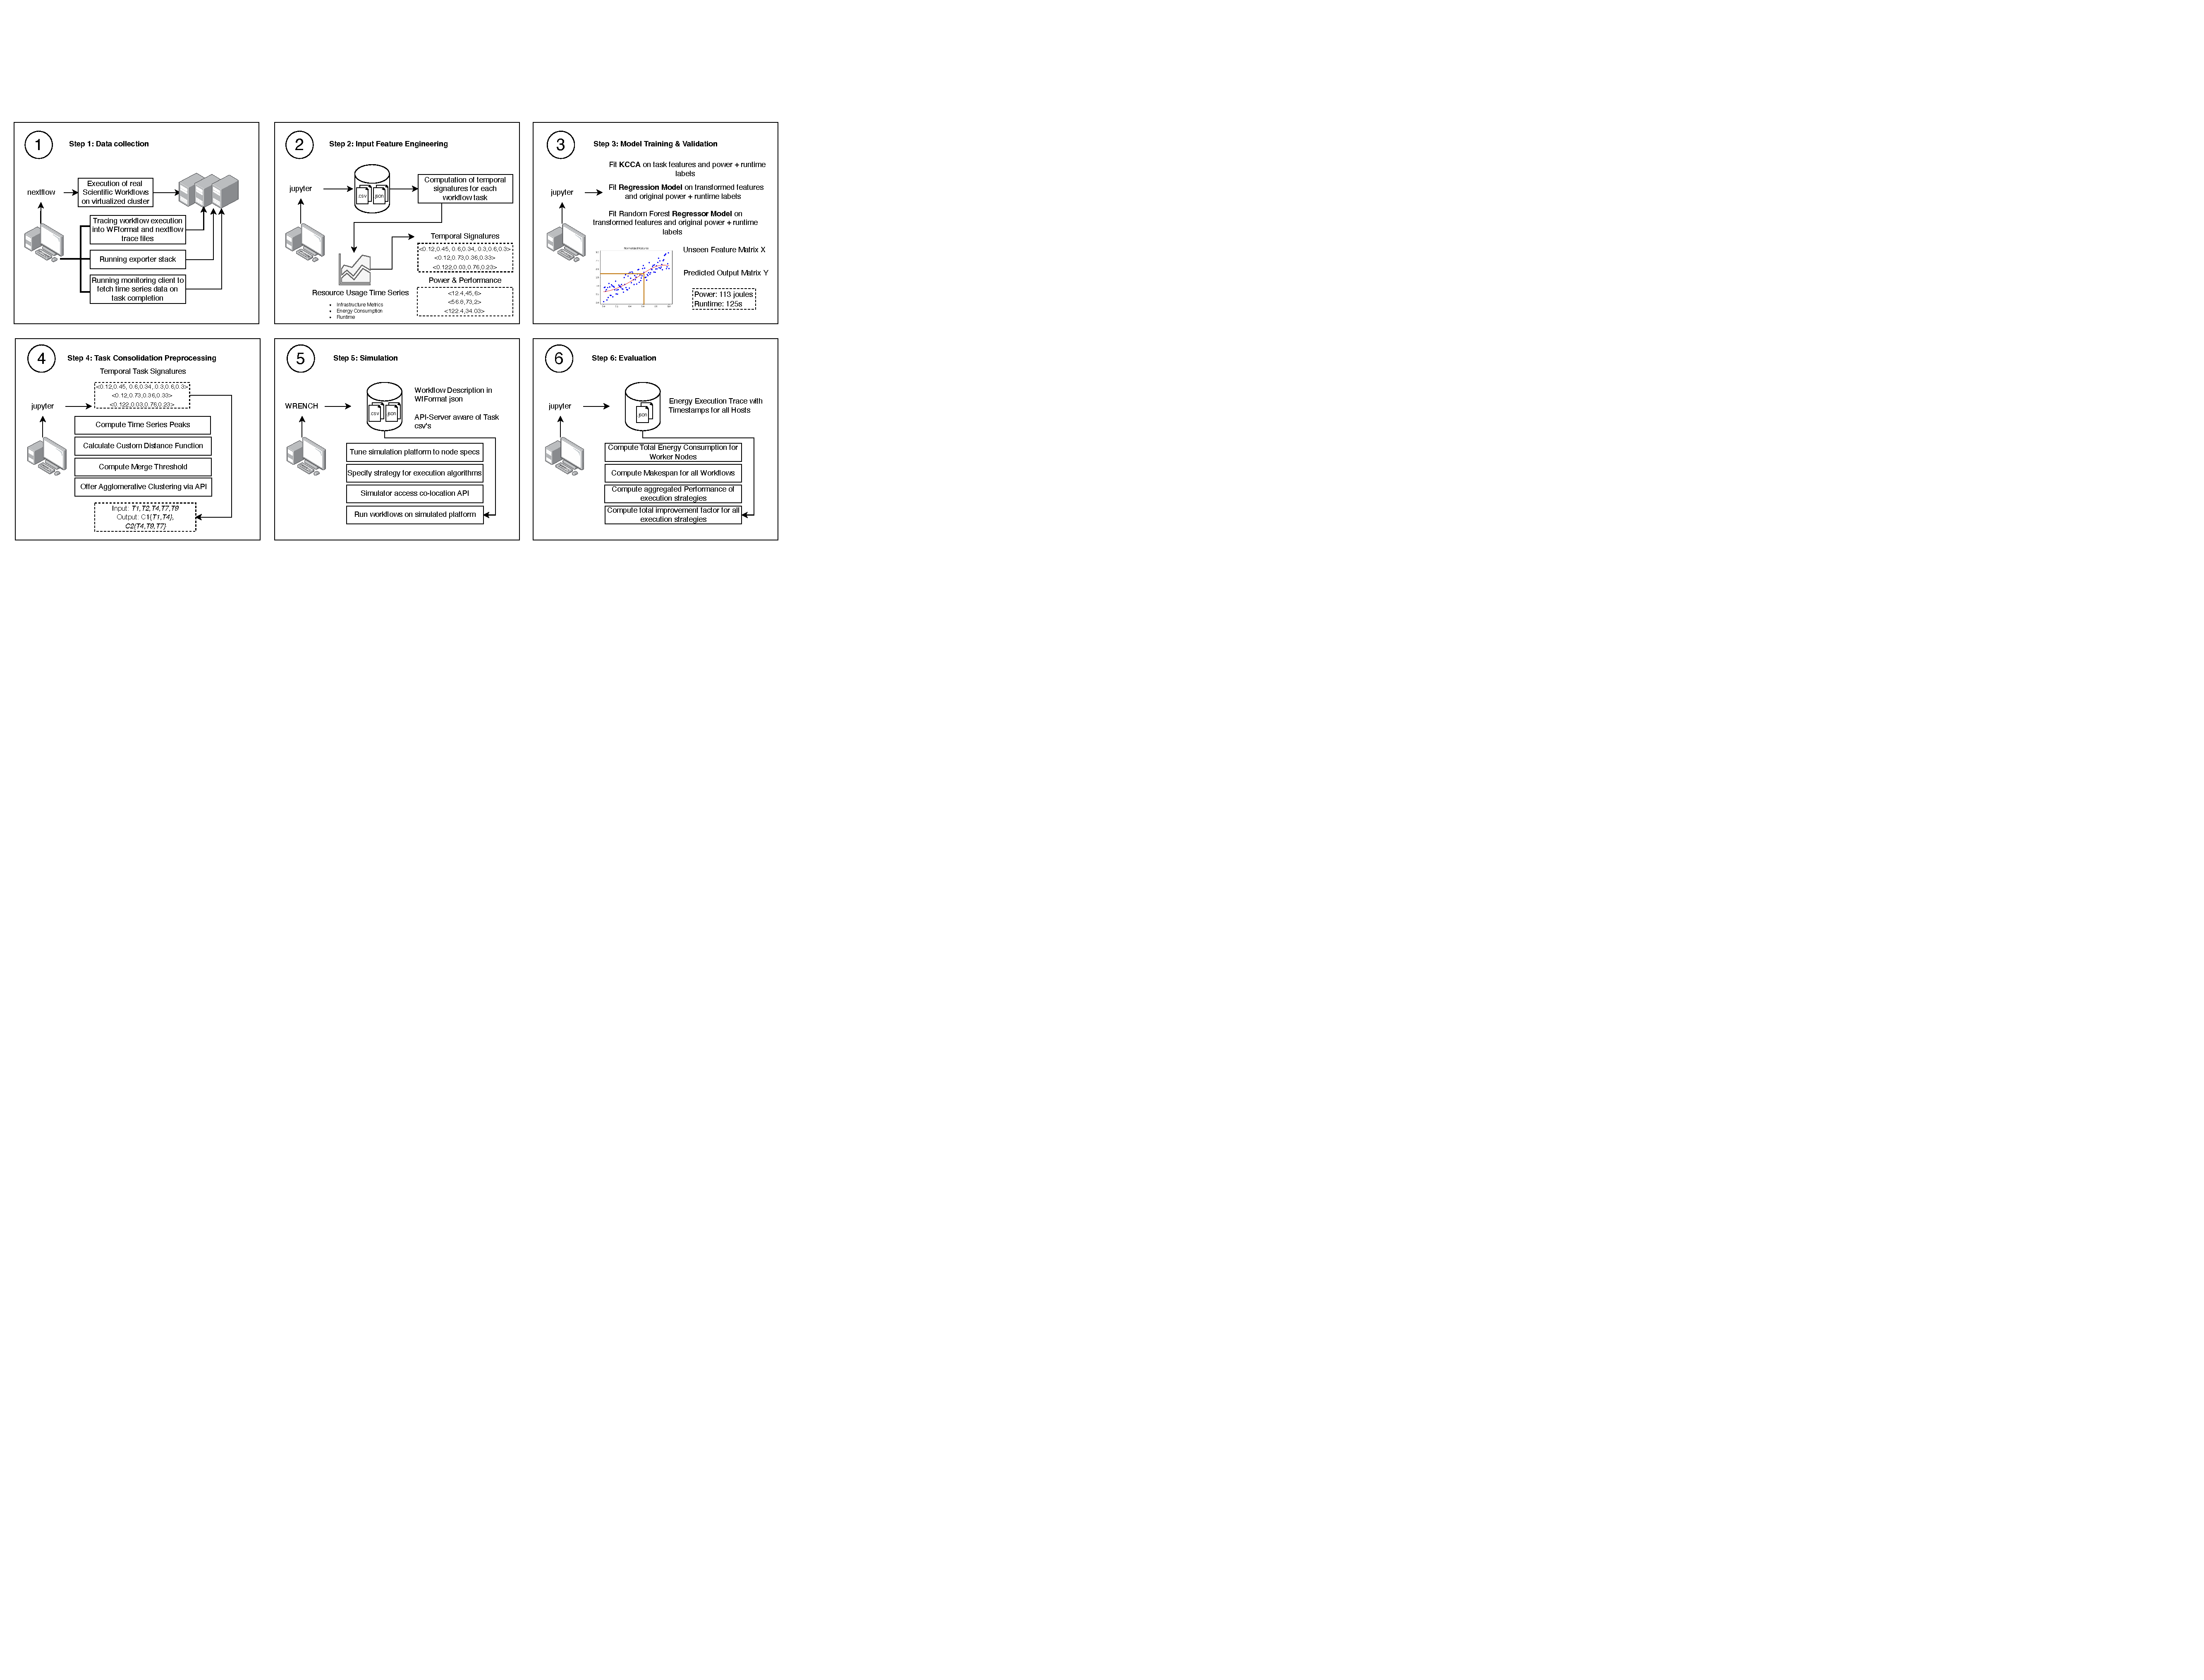
\includegraphics[scale=0.45]{fig/04/04-overview.pdf}
    \small
    \caption{Overview}
    \label{fig:04-overview}
    \tiny
    Das ist eine Beschreibung der Abbildung.
\end{figure}

The proposed research problem, introduced in Section \ref{subse:problem_motivation_description}, is decomposed into six main steps, as illustrated in Figure \ref{fig:04-overview}. Step 1, described in Section \ref{sec:online_task_monitoring}, involves a data collection phase that captures detailed execution metrics from scientific workflow runs. In Step 2, this collected data undergoes structural processing and formatting to extract relevant performance characteristics, as outlined in Section \ref{sec:data_preprocessing_general}. The raw data treatment of Step 2 is performed immediately after data collection, while Steps 3 and 4 require more specialized data preparation tailored to their respective analytical goals. Details for these stages are provided in Sections \ref{sec:data_preprocessing_clustering} and \ref{sec:data_preprocessing_predictive}.
Step 3 focuses on consolidating time-series data by identifying tasks with complementary resource usage patterns through clustering, as discussed in Section \ref{sec:task_clustering}. Step 4 reorganizes the data collected in Step 1 into a format suitable for learning the relationship between task behavior, runtime, and energy consumption, as described in Section \ref{sec:prediciton_kcca_rfr}. Finally, Steps 5 and 6, presented in Section \ref{sec:simulation_environment}, demonstrate how the theoretical concepts developed in Step 3 can be applied during workflow execution and how their potential benefits in terms of performance and energy efficiency can be evaluated through simulation.

% Assumptions or Disclaimers
\subsubsection{Assumptions}
\label{sec:assumptions}

To outline the scope, boundaries, and methodological constraints of this work, the following guiding assumptions were defined:

\begin{enumerate}
    \item \textbf{Monitoring Configuration Limits}:  Workflow tasks are described by 80 monitoring features. This work does not investigate the influence of monitoring data dimensionality on clustering and predictive performance.
    \item \textbf{Monitoring Data Coverage}: Short-lived tasks under one second are only partially captured or occasionally missed due to high system load and sampling intervals exceeding one second during workflow execution.
    \item \textbf{Offline Data Analysis}: The data preprocessing and predictive model fitting are performed offline after workflow execution. The co-location clustering algorithm is evaluated offline but also transformed into a suitable format for integration into the simulation environment.
    \item \textbf{Simulation Environment and Platform Equivalence}: The simulated platform is assumed to approximate the physical execution environment. It is expected that the overall behavior observed in simulation aligns with real-world execution trends.
    \item \textbf{Simulation Capabilities and Contention Modelling}: The WRENCH framework currently supports simulation of memory contention by limiting per-Host memory consumption, where exceeding the limit results in extended task execution times. Similarly, CPU contention is modeled through proportional increases in task runtime. Other low-level contention effects like cache interference, interconnect bottlenecks, or I/O contention are not modeled in this iteration. The energy model provided by SimGrid is assumed to realistically approximate energy consumption variations when tasks with differing resource usage profiles are co-located on the same virtual machine. The impact on energy efficiency is attributed to CPU utilization behavior and derived from the platform description where different load levels map to consumed energy amount.
\end{enumerate}

\subsection{Online Task Monitoring}
\label{sec:online_task_monitoring}

The online task monitoring approach builds on a hierarchical architecture designed to capture a broad range of metrics relevant to the execution of scientific workflows. Its design is inspired by \cite{Bader_2022} and follows a four-layered structure comprising the Resource Manager, Workflow, Machine, and Task layers. Each layer represents a distinct level of abstraction within the workflow execution environment, providing insights into specific aspects of system performance and resource utilization.

Table \ref{tab:workflow_results} provides an overview of the tools and data collection options considered to achieve these monitoring objectives, outlining how different metrics could be gathered and integrated across the hierarchical layers to form a comprehensive view of workflow behavior.

\begin{table}[H]
    \centering
    \renewcommand{\arraystretch}{1.15}
    \resizebox{\textwidth}{!}{
        \begin{tabular}{
            p{4cm}
            >{\centering\arraybackslash}p{1.8cm}
            >{\centering\arraybackslash}p{1.8cm}
            >{\centering\arraybackslash}p{1.8cm}
            >{\centering\arraybackslash}p{1.8cm}
            >{\centering\arraybackslash}p{1.8cm}
            >{\centering\arraybackslash}p{1.8cm}
            >{\centering\arraybackslash}p{1.8cm}
            }
            \toprule
            \textbf{Metric Category}         & \textbf{cAdvisor} & \textbf{Deep-Mon} & \textbf{docker-activity} & \textbf{scaphandre} & \textbf{slurm-exporter} & \textbf{process-exporter} & \textbf{cgroups-exporter} \\
            \midrule

            \multicolumn{8}{l}{\textbf{Workflow-Level Metrics}}                                                                                                                                                         \\[3pt]
            Infrastructure status            &                   &                   &                          &                     & x                       &                           &                           \\
            Running workflows                &                   &                   &                          &                     & x                       &                           &                           \\
            Workflow ID                      &                   &                   &                          &                     & x                       &                           &                           \\
            File system status               &                   &                   &                          &                     & x                       &                           &                           \\

            \midrule
            \multicolumn{8}{l}{\textbf{Machine-Level Metrics}}                                                                                                                                                          \\[3pt]
            Status                           &                   &                   &                          & x                   & x                       &                           &                           \\
            Machine type                     &                   &                   &                          & x                   & x                       &                           &                           \\
            Hardware specification           &                   &                   &                          & x                   & x                       &                           &                           \\
            Available resources              &                   &                   &                          & x                   & x                       &                           &                           \\
            Used resources                   &                   &                   &                          & x                   & x                       &                           &                           \\
            Requested and consumed resources &                   &                   &                          & x                   & x                       &                           & x                         \\
            Resource usage metrics           &                   &                   &                          & x                   & x                       &                           & x                         \\
            Power consumption                &                   &                   &                          & x                   & x                       &                           &                           \\
            Fault diagnosis                  &                   &                   &                          &                     & x                       &                           &                           \\

            \midrule
            \multicolumn{8}{l}{\textbf{Task-Level Metrics}}                                                                                                                                                             \\[3pt]
            Task status                      & x                 & x                 &                          & x                   & x                       &                           &                           \\
            Task ID                          &                   &                   &                          &                     & x                       &                           & x                         \\
            Task duration                    & x                 & x                 &                          & x                   & x                       &                           &                           \\
            Requested and consumed resources & x                 & x                 & x                        & x                   & x                       &                           & x                         \\
            Resource usage metrics           & x                 & x                 & x                        & x                   & x                       &                           & x                         \\
            Process metrics                  &                   & x                 &                          & x                   &                         & x                         &                           \\
            Power consumption                &                   & x                 & x                        & x                   & x                       &                           &                           \\

            \bottomrule
        \end{tabular}
    }
    \small
    \caption{Overview of monitored metrics and their data sources.}
    \label{tab:monitoring_sources_updated}
\end{table}
To enable access to detailed performance metrics in time-series format, Prometheus was selected as the central time-series database. As shown in Table \ref{tab:monitoring_sources_updated}, the monitoring setup therefore focused on tools that are interoperable with Prometheus as data exporters and that operate effectively within the layered monitoring framework.
During the evaluation of several potential exporters, some were excluded due to limited compatibility, excessive overhead, or incomplete metric coverage—particularly for short-lived or multi-process workflow tasks. After comparative testing, the combination of \textit{cAdvisor} and a custom fork of the DEEP-mon system \cite{8425477} produced the most stable and comprehensive results across varying workloads and resource types. These two tools were therefore selected as the foundation of the final monitoring setup.

The following table presents the final selection of data sources that were retained for the monitoring setup, along with the specific metrics enabled for each source.

% Table with Tool Overview and metrics
\begin{table}[H]
    \centering
    \renewcommand{\arraystretch}{1.2}
    \setlength{\tabcolsep}{8pt}
    \small
    \begin{tabularx}{\textwidth}{
            >{\raggedright\arraybackslash}X
            >{\raggedright\arraybackslash}X
        }
        \toprule
        \textbf{Software Tool} & \textbf{Used Metrics} \\
        \midrule

        nextflow               &
        trace file summary                             \\

        \midrule
        cAdvisor               &
        container\_memory\_working\_set\_bytes,
        container\_memory\_usage\_bytes,
        container\_memory\_rss,
        container\_fs\_reads\_bytes\_total,
        container\_fs\_writes\_bytes\_total,
        container\_fs\_io\_current                     \\

        \midrule
        Deep-Mon               &
        container\_memory\_working\_set\_bytes,
        container\_memory\_usage\_bytes,
        container\_memory\_rss,
        container\_fs\_reads\_bytes\_total,
        container\_fs\_writes\_bytes\_total,
        container\_fs\_io\_current,
        container\_mem\_rss,
        container\_mem\_pss,
        container\_mem\_uss,
        container\_kb\_r,
        container\_kb\_w,
        container\_num\_reads,
        container\_disk\_avg\_lat,
        container\_num\_writes,
        container\_cycles,
        container\_cpu\_usage,
        container\_cache\_misses,
        container\_cache\_refs,
        container\_weighted\_cycles,
        container\_power,
        container\_instruction\_retired                \\

        \bottomrule
    \end{tabularx}%
    \small
    \caption{Metrics for workflow monitoring components for task-level profiling}
    \label{tab:workflow_results}
\end{table}

% Description of cadvisor, ebpf-energy-monitor
cAdvisor is an open-source daemon for monitoring resource usage and performance of containers. It continuously discovers containers via Linux cgroups under the path /sys/fs/cgroup. Once started, cAdvisor subscribes to create/delete events in the cgroup filesystem, converts them to internal add/remove events, and configures per-container handlers. Metrics originate from machine-level facts parsed from /proc and /sys directories and most prominently container and process usage collected at cgroup boundaries. In practice, cAdvisor provides low-overhead, per-container telemetry.

DEEP-Mon is a per-thread power attribution method to translate coarse-grained hardware power measurements into fine-grained, thread-level energy estimates by exploiting hardware performance counters. The Intel RAPL interface provides power readings per processor package or core, but it cannot distinguish how much of that energy was consumed by each thread. DEEP-Mon bridges this gap by observing how actively each thread uses the processor during each sampling interval. It does so by monitoring the number of unhalted core cycles—a counter that measures how long a core spends executing instructions rather than idling. Since power consumption correlates almost linearly with unhalted core cycles, the fraction of total cycles attributed to each thread provides a reasonable proxy for its share of energy usage. DEEP-mon first computes the weighted cycles for each thread—combining its active cycles when alone with its proportionally reduced cycles when co-running. These weighted cycles determine how much of the total core-level RAPL energy should be assigned to that thread. The final per-thread power estimate is then derived by distributing the total measured power of each socket proportionally to the weighted cycle counts of all threads running on that socket. This approach allows DEEP-mon to infer realistic thread-level power usage even in systems with simultaneous multithreading and time-shared workloads, without modifying the scheduler or requiring any application-specific instrumentation. The DEEP-mon tool was modified in this work to export container-level metrics directly to Prometheus \cite{8425477}.

Based on the identification of relevant metrics and the selection of appropriate monitoring technologies, we designed an architectural model and an accompanying algorithm to define how the individual components interact. The resulting architecture integrates the selected exporter stack into a coherent monitoring workflow, ensuring that metric collection, event handling, and data aggregation are performed in a structured and automated manner. Figure \ref{fig:04-monitoring} provides an overview of the system components required for this setup, illustrating how they interact to realize the monitoring logic proposed in this work. The technical implementation details are discussed in Section \ref{cha:implementation}.

\begin{figure}[H]
    \centering
    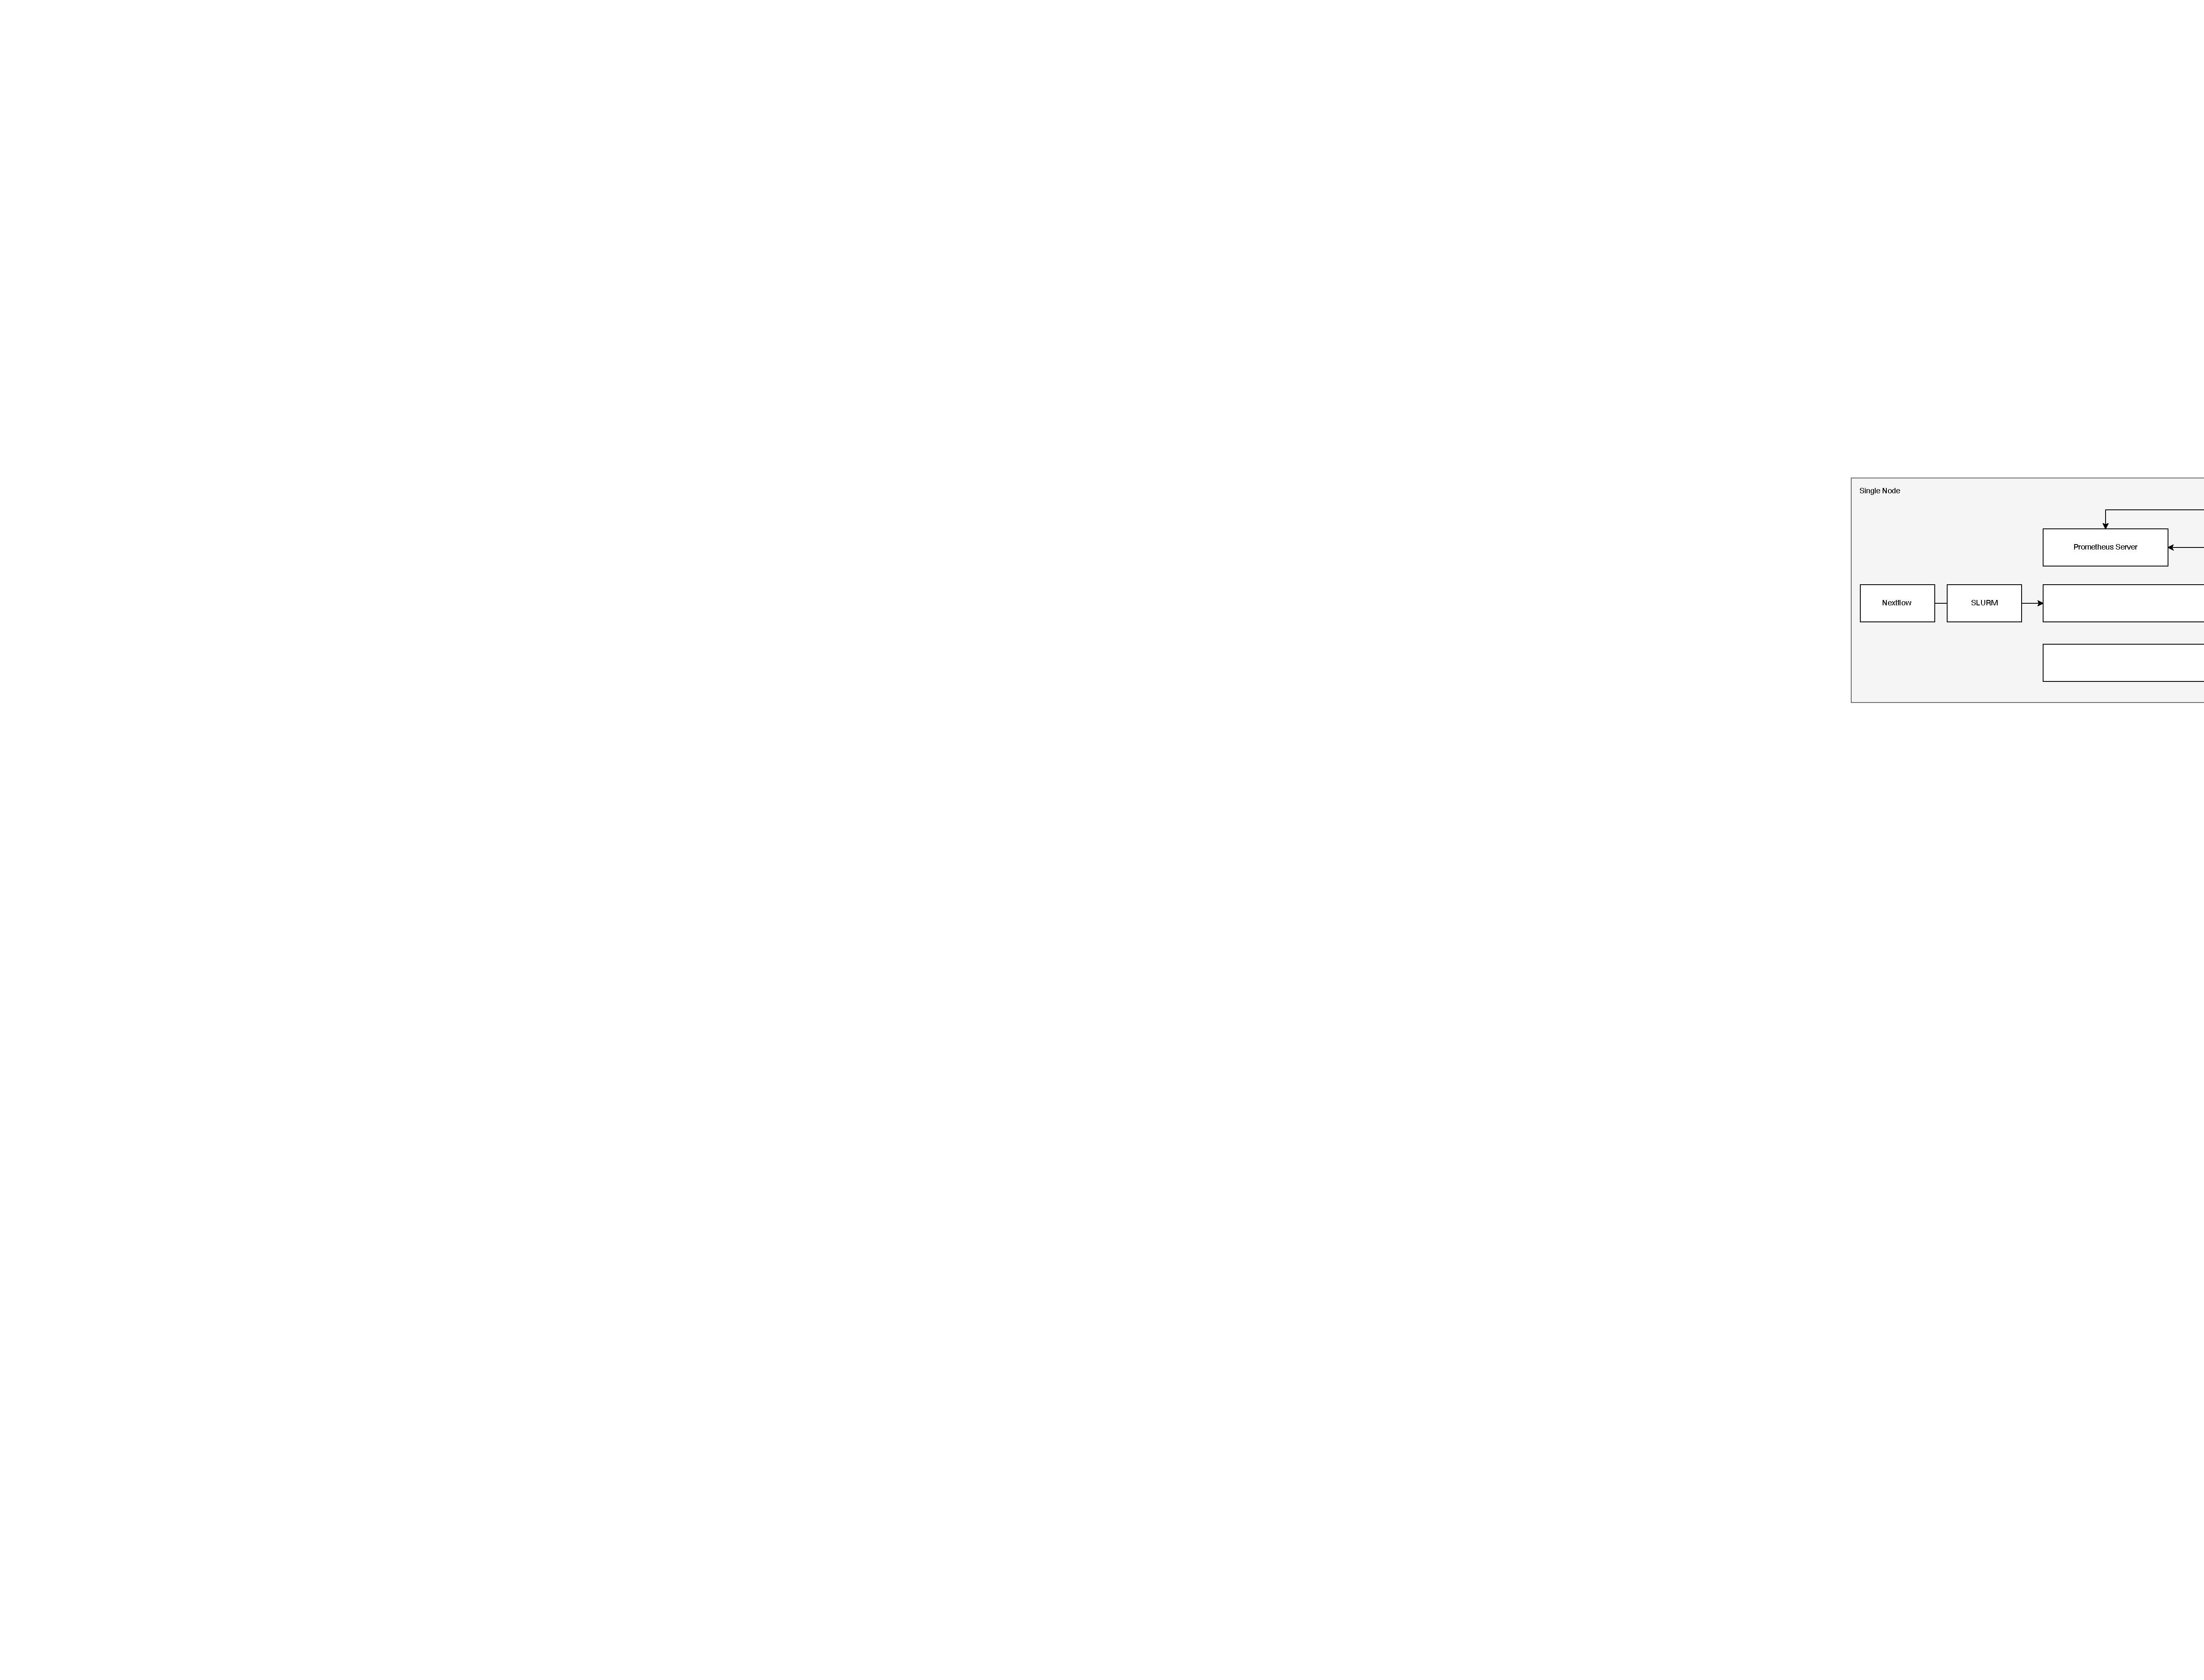
\includegraphics[scale=0.45]{fig/04/04-monitoring.pdf}
    \small
    \caption{Monitoring Client}
    \label{fig:04-monitoring}
    \tiny
    Schematic Overview of the Components of the Monitoring Client.
\end{figure}

\ref{fig:04-monitoring} and \ref{alg:monitoring} show the behavior of the monitoring client. The event listener continuously observes container lifecycle events—such as start and termination—emitted by the runtime environment. Once an event is detected, the data query interface dynamically formulates PromQL queries based on the configuration and metadata of the affected container. These queries are sent to Prometheus to retrieve fine-grained time-series data. The retrieved raw metrics are then passed to the aggregation module, which aligns and consolidates them into a unified record per container.

\begin{algorithm}[H]
    \caption{Event-Driven Monitoring and Metric Aggregation Framework}
    \label{alg:monitoring}
    \KwIn{Configuration $C$ defining monitoring targets}
    \KwOut{Aggregated container-level time-series metrics for each Nextflow process}

    \BlankLine
    initialize\_monitoring(C)\\
    init\_event\_listener()\\
    \While{true}{
        event $\gets$ wait\_for\_container\_event()\\
        meta $\gets$ extract\_metadata(event)\\
        \If{event.type = START}{
            register\_process(meta.id, meta.workflow\_label)
        }
        \If{event.type = TERMINATE}{
            metrics $\gets$ \{\}\\
            \ForEach{target $\in$ C.targets}{
                query $\gets$ build\_promql(target, meta.id, meta.time\_window)\\
                metrics[target] $\gets$ execute\_prometheus\_query(query)
            }
            data $\gets$ aggregate(metrics, meta.workflow\_label)\\
            store(data)
        }
    }
\end{algorithm}

% Algorithm Description
The algorithm outlined in Algorithm \ref{alg:monitoring} is designed to minimize monitoring overhead while ensuring that only relevant data is collected during workflow task execution. When a container start event is detected, the monitoring client extracts essential metadata—such as the container ID, the associated workflow label, and the start timestamp—and registers this information in an internal mapping to maintain a link between container identifiers and workflow tasks. When a termination event occurs, the client initiates a targeted data collection phase, querying only the relevant metrics for the specific container and execution period.

This event-driven approach ensures efficient monitoring by restricting data retrieval to the active lifecycle of workflow tasks. Furthermore, the monitoring client supports dynamic configuration of the metrics listed in Table \ref{tab:monitoring-features}, allowing users to define which metrics are collected and analyzed. This flexibility enables fine-grained, task-specific monitoring while maintaining low overhead and adaptability to different experimental requirements.

\subsection{Modelling the Co-location of Task Behavior based on Time-Series}
\label{sec:data_analysis}

This section corresponds to Steps 2,3, and 4 in Figure \ref{fig:04-overview} and explains how the collected monitoring data is transformed into structured representations of task behavior. The focus lies on preparing and processing the raw time-series metrics to generate meaningful feature sets that can be used for two main purposes: identifying complementary tasks for co-location through clustering and building predictive models that capture the relationship between task behavior, runtime, and energy consumption.

\myparagraph{General Preprocessing of Raw Time-Series Data}
\label{sec:data_preprocessing_general}

The collected monitoring data is obtained as raw time-series files in CSV format and must therefore undergo several preprocessing steps before further analysis. The goal of this stage is to transform heterogeneous monitoring outputs into a consistent and structured representation that links system-level metrics to individual workflow tasks. The general preprocessing workflow includes the following steps:

% Paragraph about generic preprocessing of raw data
\begin{enumerate}
    \item Parsing of raw time-series CSV files.
    \item Alignment of timestamps across different sources.
    \item Merging of per-task data into unified records.
    \item Matching Entities between execution layer and workflow layer
\end{enumerate}

% TODO: Add cursive for entities
% Explaining the pre-processing
During workflow execution, data is produced at multiple abstraction levels—from the resource manager down to container metrics. To transform this heterogeneous data into a unified, task-level format, a structured preprocessing pipeline was developed. First, all monitoring outputs are recursively traversed and scoped according to the desired data sources and metric types. The resulting directory tree is then filtered to retain only relevant metrics, such as task metadata and power measurements. Each dataset is subsequently split into per-task CSV files based on container identifiers.
As an anchor for this process, the started and died container tracking files are used, which record general container lifecycle information such as container names, identifiers, and timestamps. To establish a consistent mapping between workflow tasks and their corresponding container traces, entity matching is performed. Here, container lifecycle records—capturing task identifiers, container names, and working directories—serve as the linking mechanism between workflow-level entities and container-level monitoring data. The working directories are attached to every container trace, enabling a reliable cross-reference with workflow metadata extracted from Nextflow trace files. This ensures that each monitored container is correctly associated with the corresponding workflow task, providing a coherent, task-centric dataset for subsequent analysis.

\subsubsection{Task Clustering for Contention-Aware Consolidation}
\label{sec:task_clustering}

Following the preprocessing and structuring of raw time-series data, we continue to address step 3 of the overall approach outlined in \ref{fig:04-overview}. This step focuses \textit{ShaReComp's} mechanics - task clustering as a means of identifying tasks that can be co-located without causing severe resource contention. The goal is to refine the processed monitoring data into representations that capture each task's characteristic resource usage patterns and to use these representations for forming complementary task groups. This clustering step forms the conceptual foundation for contention-aware consolidation

\myparagraph{Preprocessing Raw Time-Series Data for Task-Clustering}
\label{sec:data_preprocessing_clustering}

To prepare the data for contention-aware task clustering, the processed time-series must be transformed into a compact yet expressive representation of each task's resource usage behavior. This ensures that the clustering algorithm can meaningfully capture similarities and differences between tasks across multiple resource domains. We therefore apply the following two main preprocessing steps prior to executing the clustering algorithm.

\begin{enumerate}
    \item \textbf{Peak-pattern construction}. For every task and monitored workload type, we first derive a peak time series: the raw per-second resource signal is resampled into three-second buckets and the maximum per bucket is retained. When two peak series must be compared, we truncate both to the shorter length so that correlation is computed on aligned vectors without padding artifacts.
    \item \textbf{Computing Workload-type affinity}. Different resource domains interfere to different degrees such as CPU vs CPU peaks are typically more contentious than CPU vs file I/O. We encode this by computing an affinity score between workload types which is described in \ref{sec:measuring_resource_contention}. High affinity means higher potential interference when peaks align; low affinity reflects benign coexistence.
\end{enumerate}

While the first step focuses on constructing consistent temporal representations of task behavior, the second step introduces a quantitative measure of how different workload types interact when co-located. To provide a clearer understanding of this relationship and its role in the clustering process, we examine the computation of workload-type affinity in more detail.

% Workload experiment design
\myparagraph{Measuring Resource Interference of Co-located Benchmarks}
\label{sec:measuring_resource_contention}

The measurement of resource contention follows a two-stage protocol that first establishes isolated baselines for each workload class and then repeats the same workloads under controlled co-location. In the baseline stage, CPU-bound, memory-bound, and file-I/O-bound benchmark containers are executed one at a time on pinned logical CPUs. Each run records a start and finish timestamp at microsecond resolution. In parallel, Deep-Mon is used to record the power time series for each container. After a run finishes, the power streams of the containers are retained, aligned to the containers lifetime, and summarized to a representative mean value.
After isolated benchmark execution we replay the same benchmarks in pairs to expose interference effects by CPU pinning. The experiment binds pairs of benchmarks to siblings on the same physical core to amplify shared-core effects. Each co-located container is measured in exactly the same way as in isolation, producing a matched set of durations and power summaries.

% Notation for the experiments.
In order to derive a workload affinity from the contention experiments we define contention effects to occur when co-located workloads exceed their duration and power consumption compared to their isolated measurements.
\[
    \textbf{Isolated and Co-located Metrics}
\]

For each workload \( i \in \{1,2\} \), let
\[
    t_i^{(iso)}, \; t_i^{(coloc)} \quad \text{denote the isolated and co-located runtimes,}
\]
\[
    P_i^{(iso)}, \; P_i^{(coloc)} \quad \text{denote the average isolated and co-located power consumption.}
\]

\[
    \textbf{Per-workload Slowdown Factors}
\]

The per-workload slowdowns are defined as
\[
    S_i^{(t)} = \frac{t_i^{(coloc)}}{t_i^{(iso)}},
    \qquad
    S_i^{(P)} = 1 + \log\!\left(
    \max\!\left( \frac{P_i^{(coloc)}}{P_i^{(iso)}}, 1 \right)
    \right),
\]
ensuring that both runtime and power slowdowns are
non-negative and at least one in value.

The mean slowdowns across the workload pair are
\[
    \bar{S}^{(t)} = \frac{S_1^{(t)} + S_2^{(t)}}{2},
    \qquad
    \bar{S}^{(P)} = \frac{S_1^{(P)} + S_2^{(P)}}{2}.
\]

A weighted average combines both effects:
\[
    \bar{S} =
    \alpha\, \bar{S}^{(t)} + (1 - \alpha)\, \bar{S}^{(P)},
    \quad \text{with } \alpha \in [0,1],
\]
where higher \(\alpha\) emphasizes runtime effects,
and lower \(\alpha\) gives more weight to power efficiency.

The final combined slowdown factor is
\[
    \bar{S}_{\text{final}} = \max(1, \bar{S}),
\]
guaranteeing that co-location never yields an apparent
speedup (values \(\ge 1\) indicate slowdown).

\[
    \textbf{Affinity Score}
\]

The affinity score \(A\) quantifies the degree of
interference between two co-located workloads.

First, compute pairwise affinity ratios:
\[
    A^{(t)} =
    \frac{t_1^{(coloc)} + t_2^{(coloc)}}
    {t_1^{(iso)} + t_2^{(iso)}},
    \qquad
    A^{(P)} =
    1 + \log\!\left(
    \max\!\left(
    \frac{P_1^{(coloc)} + P_2^{(coloc)}}
    {P_1^{(iso)} + P_2^{(iso)}},
    1
    \right)
    \right).
\]

A weighted average combines both effects:
\[
    A_{\text{raw}} =
    \alpha\, A^{(t)} + (1 - \alpha)\, A^{(P)},
    \qquad A_{\text{raw}} \ge 1.
\]

The normalized affinity score is then:
\[
    A =
    \frac{1 - \frac{1}{A_{\text{raw}}}}{\beta},
    \qquad A \in [0, 1],
\]
where \(\beta > 0\) controls scaling sensitivity.
Values of $A \approx 0$ indicate minimal interference,
while \(A \to 1\) signifies strong co-location interference.


\myparagraph{Algorithmic Approach to Task Consolidation}
\label{sec:algorithmic_approach_consolidation}

Building on the previously derived peak time-series representations and the computed workload-type affinity scores, we propose an algorithmic formulation of the clustering, or consolidation, process.
Consolidation is formulated as a clustering problem with an important modification: rather than grouping tasks that are similar, the goal is to cluster tasks with complementary resource usage patterns to minimize contention during co-location. Building on the previously established notion of affinity—which quantifies how strongly workloads interfere when sharing resources—the clustering process incorporates this measure directly into its distance metric. The distance between tasks increases when two tasks exert pressure on the same resources simultaneously, indicating potential contention, and decreases when their resource usage peaks complement one another.

Algorithm \ref{alg:task_distance_clustering} showcases the \textit{ShaReComp} task consolidation procedure developed in this work, integrating both the peak-pattern representations and affinity scores into a unified clustering process. The method first computes pairwise similarities between all task signatures, where each signature encodes the temporal evolution of multiple resource metrics. These similarities are weighted by the experimentally derived affinity values to reflect the degree of potential interference between workloads. The resulting similarity matrix thus provides a contention-aware view of task compatibility.
A percentile-based threshold is then applied to adaptively determine the stopping condition for cluster formation, ensuring that only task pairs with sufficiently low contention potential are merged. Finally, agglomerative clustering is executed using average linkage criterion to form consolidated task groups that exhibit complementary resource utilization.

% Algorithm for Task Consolidation in ShaReComp
\begin{algorithm}[H]
    \caption{ShaReComp - Task Consolidation Algorithm}
    \label{alg:task_distance_clustering}
    \SetKwFunction{Sim}{compute\_similarity}
    \SetKwFunction{Thresh}{percentile\_threshold}
    \SetKwFunction{Merge}{agglomerative\_merge}

    \KwIn{task signatures $\mathrm{sig}$, affinity weights $w$, percentile $\tau$, linkage}
    \KwOut{clusters $\mathcal{C}$}

    $S \gets$ \Sim($\mathrm{sig}$, $w$) \tcp*[r]{resource-aware similarity}
    $\theta \gets$ \Thresh($S$, $\tau$) \tcp*[r]{percentile-based stopping rule}
    $\mathcal{C} \gets$ \Merge($S$, $\theta$, linkage) \tcp*[r]{agglomerative clustering}

    \textbf{return } $\mathcal{C}$
\end{algorithm}

We examine each stage of Algorithm~\ref{alg:task_distance_clustering} in turn.

\textbf{Anti-similarity distance.} For any pair of tasks i,j, we iterate over their workload types and use two factors: (i) the affinity between the two types; (ii) the correlation between their corresponding peak series computed twice, once per type, to capture both sides of the pairing. We then aggregate these terms so that highly correlated peaks in high-affinity domains increase the distance, whereas low or negative correlations in low-affinity pairs decrease it. The result is a symmetric task distance matrix whose off-diagonal entries quantify how bad it would be to co-locate the two tasks, and whose diagonals are zero by definition.

% Notation for the distance formula
\[
    \textbf{Inter-Task Distance and Resource Correlation Model}
\]

To quantify the similarity and potential contention between two workloads
\( i \) and \( j \), we define a composite distance measure
that integrates both resource affinity and correlation of peak usage.
Each workload utilizes a set of resources
\( R = \{ \text{CPU}, \text{Memory}, \text{Disk}\} \),
yielding in total ten pairwise combinations of resource types across two tasks.
The distance term combines the precomputed affinity score with the
correlation of peak resource intensities.

\[
    D_{i,j}
    = \sum_{R_1, R_2}
    \Bigl(
    (\mathrm{aff\text{-}score}(R_1^i, R_2^j))
    \cdot
    \mathrm{Corr}(\mathrm{peak}\,R_1^i, \mathrm{peak}\,R_1^j)
    \cdot
    \mathrm{Corr}(\mathrm{peak}\,R_2^i, \mathrm{peak}\,R_2^j)
    \Bigr)
    \tag{1}
\]

where:
\begin{align}
    R_1^i, R_2^j & \; \text{denote resource types of workloads } i \text{ and } j,                           \\[4pt]
    \mathrm{Corr}(\mathrm{peak}\,R_1^i, \mathrm{peak}\,R_1^j)
                 & \; \text{is the Pearson correlation between the peak usages of resource } R_1,            \\[4pt]
    \mathrm{aff\text{-}score}(R_1^i, R_2^j)
                 & \in [0, 1] \text{ measures the degree of interference between } R_1^i \text{ and } R_2^j.
\end{align}

\[
    \textbf{Interpretation}
\]

The intuition behind this distance metric is to
\emph{promote dissimilar task pairings} for co-location.
If two workloads exhibit highly correlated peak usage on the same resources,
their corresponding correlation terms will be large,
thus increasing \( D_{i,j} \) and discouraging their co-location.
Conversely, tasks with uncorrelated or complementary resource peaks
yield smaller distance values and are therefore more suitable to merge.

The affinity score modulates this behavior:
smaller values of \( \mathrm{aff\text{-}score} \)
indicate lower interference between resource pairs,
which can offset strong peak correlations.

Finally, clustering proceeds by iteratively merging task clusters
whose inter-cluster distance satisfies:
\[
    D_{i,j} < \text{merge\_threshold}.
\]
This ensures that only compatible workloads, in terms of both
resource affinity and temporal peak correlation, are grouped together.

\textbf{Computing the merge threshold}. Because the distance matrix is data-dependent, we estimate a merge threshold directly from its empirical distribution. In our appraoch we select the 20th percentile on the raw distances as an automatic cut-level: any pair below this threshold is safe enough to consider for co-location, while pairs above it are kept apart.

\textbf{Agglomerative clustering with precomputed distances}. We run average-linkage agglomerative clustering on the precomputed distance matrix with the chosen distance threshold and no preset cluster count. This yields variable-sized clusters whose members are mutually non-contentious under our metric. Because we use a threshold rather than a fixed k, the method adapts to each workload mix, producing more or fewer groups as warranted by the observed interference structure.

% I think it's discussed somewhere else.
% \textbf{From clusters to co-location candidates}. Each cluster defines a candidate co-location set. To make these cluster-level entities usable by predictive models discussed in \ref{sec:prediciton_kcca_rfr}, we construct cluster feature vectors by flattening and concatenating the per-task temporal signatures of all members and summing them dimension-wise. This potentially approximates the combined load shape we would see if the clusters tasks were executed in a co-located manner.


\subsubsection{Predicting the Runtime and Energy Consumption of Task Clusters}
\label{sec:prediciton_kcca_rfr}

Following the reasoning of \cite{5644899}, we investigate whether the formed task clusters exhibit shared structures in terms of correlations between their time-series behavior and their corresponding energy and performance metrics. To this end, we adopt their proposed approach for preprocessing time-series data into temporal signatures on a per-task basis.

\myparagraph{Preprocessing Raw Time-Series Data for Predictive Modelling}
\label{sec:data_preprocessing_predictive}

Unlike the preprocessing described in Section \ref{sec:data_preprocessing_clustering}, the following procedure prepares the data specifically for step 4 of the overall approach shown in Figure\ref{fig:04-overview}, focusing on transforming raw time-series inputs into a form suitable for predictive modeling.

\begin{enumerate}
    \item Temporal signature construction.
          \subitem Sampling and smoothing.
          \subitem Equal-length normalization.
          \subitem Container-wise collation.
    \item Model Input Construction.
          \subitem Normalization and Scaling.
          \subitem Extraction of Input Features and Output Labels.
\end{enumerate}

% Formal notation

\[
    \textbf{Temporal Signature and Model Input Construction}
\]

We denote by \( \mathcal{T} = \{ T_1, T_2, \dots, T_N \} \) the set of
temporal signatures extracted from the monitored resource-usage profiles
of \( N \) workflow tasks.
Each task \( i \) is characterized by time-varying utilization traces
for the monitored resource dimensions
\[
    R = \{ \text{CPU}, \text{Memory}, \text{Disk} \}.
\]

\noindent
For each resource \( r \in R \) and task \( i \),
the temporal signature \( T_i^{(r)} \) is defined as a
coarse-grained summary of the normalized resource usage signal
\( x_i^{(r)}(t) \):
\[
    T_i^{(r)} =
    \bigl\langle
    p_{1,i}^{(r)},\;
    p_{2,i}^{(r)},\;
    \dots,\;
    p_{10,i}^{(r)}
    \bigr\rangle,
    \tag{1}
\]
where each component \( p_{k,i}^{(r)} \) represents the mean
usage value within segment \( k \) of the time-normalized
execution window (\( k = 1, \dots, 10 \)).
This yields a ten-dimensional vector describing the temporal pattern of
resource consumption.

\noindent
The feature vector for task \( i \) is obtained by concatenating
the resource-specific signatures:
\[
    x_i =
    \bigl[
    T_i^{(\text{CPU})},\;
    T_i^{(\text{Memory})},\;
    T_i^{(\text{Disk})},\;
    \bigr]
    \in \mathbb{R}^{d_x},
\]
where \( d_x = 3 \times 10 = 30 \) in this example configuration.

\[
    X =
    [x_1^\top, x_2^\top, \dots, x_N^\top]^\top
    \in \mathbb{R}^{N \times d_x}
\]
denotes the complete input matrix used for model training.

Similarly, for each task \( i \), the execution-level targets
(time and mean power consumption) are given by
\[
    y_i = [\,t_i,\, P_i\,] \in \mathbb{R}^2,
    \quad
    Y = [y_1^\top, y_2^\top, \dots, y_N^\top]^\top
    \in \mathbb{R}^{N \times 2}.
\]

\[
    \textbf{Example}
\]
Consider \( N = 3 \) workflow tasks with simplified
CPU and memory usage signatures
(each consisting of 3 representative pattern points for brevity):
\[
    \begin{array}{lcccccc}
        \toprule
        \text{Task}        &
        p_1^{(\text{CPU})} & p_2^{(\text{CPU})} & p_3^{(\text{CPU})} &
        p_1^{(\text{Mem})} & p_2^{(\text{Mem})} & p_3^{(\text{Mem})}                             \\
        \midrule
        1                  & 0.40               & 0.75               & 0.90 & 0.35 & 0.55 & 0.60 \\
        2                  & 0.20               & 0.50               & 0.70 & 0.25 & 0.40 & 0.50 \\
        3                  & 0.30               & 0.65               & 0.85 & 0.30 & 0.45 & 0.55 \\
        \bottomrule
    \end{array}
\]

Concatenating these signatures yields the input matrix
\[
    X =
    \begin{bmatrix}
        0.40 & 0.75 & 0.90 & 0.35 & 0.55 & 0.60 \\
        0.20 & 0.50 & 0.70 & 0.25 & 0.40 & 0.50 \\
        0.30 & 0.65 & 0.85 & 0.30 & 0.45 & 0.55
    \end{bmatrix},
    \quad
    Y =
    \begin{bmatrix}
        12.4 & 65 \\
        14.1 & 72 \\
        10.8 & 58
    \end{bmatrix}.
\]

Here, each row of \( X \) encodes the temporal resource-usage pattern
of a task, while \( Y \) provides the corresponding runtime and mean
power consumption used for model learning or correlation analysis.

This preprocessing yields: (i) a standardized and fixed-length feature matrix X that preserves per-metric usage distributions and (ii) a label matrix Y capturing runtime and energy

Building upon Algorithm \ref{alg:sharecomp} in Section \ref{sec:task_clustering}, we extend the \textit{ShaReComp} concept by linking task clustering with predictive modeling. This step introduces a follow-up procedure that uses the clustered task groups and their extracted temporal features from Section~\ref{sec:prediciton_kcca_rfr} to model and predict the expected runtime and energy behavior of consolidated task clusters.

% Algorithm for prediction of task clusters.
\begin{algorithm}[H]
    \caption{ShaReComp — Prediction of Energy and Performance Behavior of Consolidated Task Clusters}
    \label{alg:sharecomp_prediction}
    \SetKwFunction{Aggregate}{sum\_cluster\_features}
    \SetKwFunction{Build}{build\_feature\_matrix}
    \SetKwFunction{Predict}{predict\_runtime\_and\_energy}

    \KwIn{task clusters $\mathcal{C}$, per-task signatures $\mathrm{sig}$, trained model $\mathcal{M}$ (KCCA or Random Forest)}
    \KwOut{predicted runtime energy pairs $\hat{Y} = \{ (\hat{t}_k, \hat{E}_k) \}$}

    \BlankLine
    \ForEach{cluster $C_k \in \mathcal{C}$}{
        $F_k \gets$ \Aggregate($\{\,\mathrm{sig}[t_i] \mid t_i \in C_k\,\}$) \tcp*[r]{sum task signatures to form cluster feature}
    }
    $X \gets$ \Build($\{F_k\}$) \tcp*[r]{construct consolidated feature matrix}

    \BlankLine
    \ForEach{cluster feature $X_k \in X$}{
        $(\hat{t}_k, \hat{E}_k) \gets$ \Predict($X_k$, $\mathcal{M}$)
    }
    \BlankLine
    \textbf{return } $\hat{Y} = \{ (\hat{t}_k, \hat{E}_k) \}_{k=1}^{|\mathcal{C}|}$
\end{algorithm}

The statistical models used in \ref{alg:sharecomp_prediction} are described in the following.

\myparagraph{Kernel Canonical Correlation Analysis}
\label{sec:KCCA}

KCCA wants to identify relationships between task-specific features and their corresponding performance and energy characteristics. To achieve this, the dataset is divided into two parts: approximately 70\% of the tasks are used for training the models, while the remaining 30\% are reserved for testing and validation.

KCCA itself does not perform prediction but rather uncovers shared structures between task feature data performance outcomes. Through the data preprocessing described in the previous step, we prepare the feature matrices so that a regression model can generalize from the learned shared space to unseen inputs—for instance, the aggregated features of a new task cluster. We use KCCA to project both input and target data into a common latent space that captures nonlinear relationships between task resource usage and performance behavior. During training, we then fit a Kernel Ridge Regression model on the latent-space representations of the input features and the original, unnormalized target values Y (runtime and energy). This approach leverages KCCA's ability to transform unseen data into the same latent space, allowing KRR to predict concrete runtime and energy values for previously unseen X inputs. KRR is chosen because, as outlined in Chapter~1, it extends ordinary least squares regression by capturing nonlinear dependencies through kernel-based feature mappings.

% Notation
To capture nonlinear dependencies between the resource signatures
and performance power outcomes, we apply Gaussian kernels to both
input and output feature spaces.

KCCA seeks directions \(A\) and \(B\) in the
reproducing kernel spaces of \(K_x\) and \(K_y\)
that maximize the correlation between
\( K_x A \) and \( K_y B \).
This is expressed as the generalized eigenvalue problem:
\[
    \begin{bmatrix}
        0       & K_y K_x \\
        K_x K_y & 0
    \end{bmatrix}
    \begin{bmatrix}
        A \\ B
    \end{bmatrix}
    =
    \lambda
    \begin{bmatrix}
        K_x^2 & 0     \\
        0     & K_y^2
    \end{bmatrix}
    \begin{bmatrix}
        A \\ B
    \end{bmatrix}.
    \tag{2}
\]

Solving (2) yields paired canonical directions
\( (A, B) \) that define latent projections
\[
    X' = K_x A, \qquad Y' = K_y B,
\]
maximally correlated across the two feature spaces.
These projections represent a shared latent space
relating resource utilization dynamics to task performance and energy.

\[
    \textbf{Illustrative Example}
\]
Consider three workflow tasks \( i = 1, 2, 3 \)
with aggregated temporal signatures over CPU and memory:
\[
    x_1 = [0.40,\, 0.75,\, 0.90,\, 0.35,\, 0.55,\, 0.60], \quad
    x_2 = [0.20,\, 0.50,\, 0.70,\, 0.25,\, 0.40,\, 0.50], \quad
    x_3 = [0.30,\, 0.65,\, 0.85,\, 0.30,\, 0.45,\, 0.55].
\]
Their corresponding runtime power outcomes are:
\[
    y_1 = [12.4,\, 65], \quad
    y_2 = [14.1,\, 72], \quad
    y_3 = [10.8,\, 58].
\]

KCCA maps both the temporal patterns \(x_i\)
and the performance power pairs \(y_i\)
into high-dimensional kernel spaces
and finds projections that maximize their mutual correlation.
In this example, the first canonical mode reveals that
tasks with higher sustained CPU activity
(\(x_1, x_3\))
correspond to lower execution time and reduced power consumption,
while the less efficient task (\(x_2\))
shows a distinct temporal signature characterized by
fluctuating utilization and higher runtime.

\myparagraph{Random Forest Regression}

To complement the KCCA model, we trained two non-parametric regressors based on Random Forests—one to predict mean task power and one to predict task runtime from the same preprocessed feature matrix. We reuse the exact same data as we did for the KCCA model as Random Forests perform well on both multivarita input and output data. The power model is trained on mean per-task energy-rate labels, while the runtime model uses task durations as targets. As a sanity check, we established simple baselines by predicting the training-set mean once for power and once for runtime on the test split. These baselines quantify the minimum improvement any learned model must exceed.

To illustrate this concept, we consider the following example.

% Example on how this looks
\myparagraph{Example on Predicting the Performance of Task Cluster with ShaReComp}
\label{sec:example_prediction_task_clusters}

Assume two clusters:
\[
    C_1 = \{t_1, t_2\}, \quad C_2 = \{t_3\},
\]
and each task has a CPU Memory signature with three pattern points:
\[
    t_1 = [0.4, 0.7, 0.9, 0.5, 0.6, 0.7], \quad
    t_2 = [0.3, 0.5, 0.8, 0.4, 0.5, 0.6], \quad
    t_3 = [0.2, 0.4, 0.6, 0.3, 0.4, 0.5].
\]
Applying \ref{alg:sharecomp_prediction} Cluster features are summed:
\[
    F_1 = t_1 + t_2 = [0.7, 1.2, 1.7, 0.9, 1.1, 1.3], \quad
    F_2 = t_3.
\]
Model predictions from both Kernel Ridge Regression or the Random Forest Regressor yield
\[
    \hat{Y} =
    \begin{bmatrix}
        10.8 & 62.5 \\
        14.2 & 75.1
    \end{bmatrix},
\]
representing predicted runtime (seconds) and energy (joules) per cluster.

\subsection{Simulation of Task Co-location during Workflow Execution}
\label{sec:simulation_environment}

We advance to steps 5 and 6 of the overall approach shown in Figure \ref{fig:04-overview}, where the previously developed concepts are embedded into a workflow execution environment. In this stage, the focus shifts from modeling and clustering individual tasks to simulating their co-location during execution, eventually allowing us to evaluate how these strategies affect overall performance and energy efficiency.

\myparagraph{Outline of Simulation Components}

\label{sec:design_pillars}
We build upon generic design pillars that structure the simulation environment.

% Figure with Simulator Design
\begin{figure}[H]
    \centering
    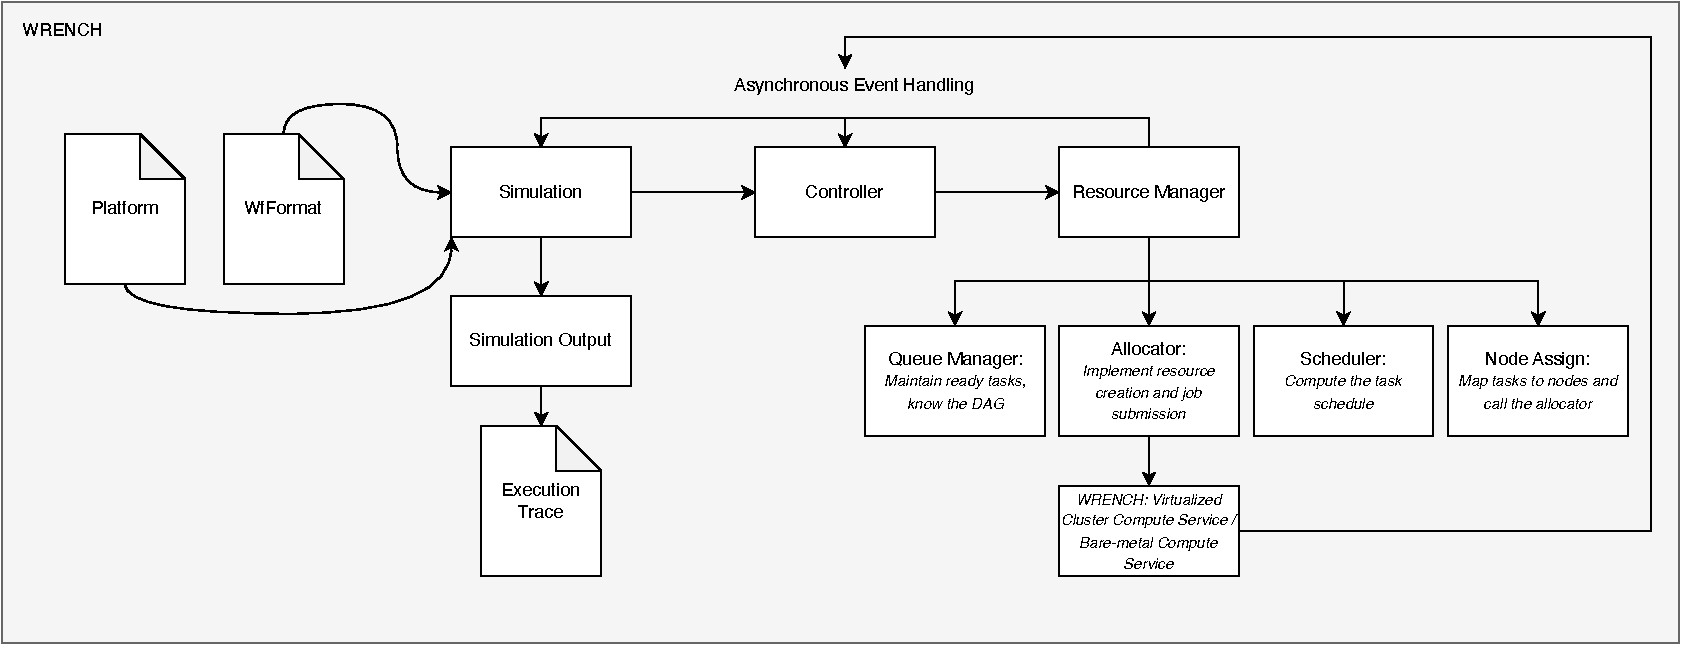
\includegraphics[scale=0.5]{fig/04/04-approach-sim.pdf}
    \small
    \caption{High-level Simulator Design}
    \label{fig:04-sim-design}
    \tiny
    Simulator Design using WRENCH for studying Energy-aware Co-location of Scientific Workflow Tasks.
\end{figure}

The design of distributed HPC systems typically revolves around three fundamental mechanisms: resource allocation, queue management and dispatching, and job placement. As illustrated in Figure \ref{fig:04-sim-design}, these principles are adapted and integrated into our simulator through a dedicated controller component that interacts with a central resource manager. This resource manager orchestrates task scheduling, DAG-aware queue handling, task-to-node assignment, and the eventual allocation and execution of tasks on compute resources. Because the objective of this work is to analyze the effects of task co-location, the simulator's processing engine is designed with extensible interfaces that support alternative scheduling, mapping, and allocation strategies—from traditional First-In-First-Out (FIFO) execution to heuristic or energy-aware methods that emphasize beneficial co-location patterns.

\subsubsection{Embedding Task Co-location into Scheduling Heuristics}
\label{sec:heuristic_design}

Our algorithmic design for the resource manager, allocator, and scheduler components shown in Figure \ref{fig:04-sim-design} follows heuristic principles. Instead of formulating co-location within the scheduling process as an explicit optimization problem, we embed it through a set of simple, interpretable decision rules. Heuristic algorithms are particularly suited for this purpose, as they enable deterministic, rule-based navigation of the scheduling space without requiring exhaustive or stochastic search, thus ensuring transparency and efficiency in evaluating co-location strategies. We divide the task-to-node mapping process into two distinct stages, as illustrated in Figure \ref{fig:04-coloc-problem}. The simulation begins by launching the controller component, which invokes the resource manager. Through its queue management mechanism, the resource manager identifies all ready-to-run tasks that have no remaining dependencies. In the depicted example, tasks 1, 2, 4, 8, 11, 12, and 15 are selected for scheduling. For this process, we adopt list-scheduling algorithms, one of the most established heuristic approaches in workflow scheduling. These algorithms assign each task a priority or ranking based on topological and performance characteristics such as critical path length, estimated execution time, or communication cost. Tasks are then scheduled iteratively, with the highest-priority unscheduled task being mapped to an available resource until all ready tasks have been assigned.

% Figure with visualizing the co-loc problem
\begin{figure}[H]
    \centering
    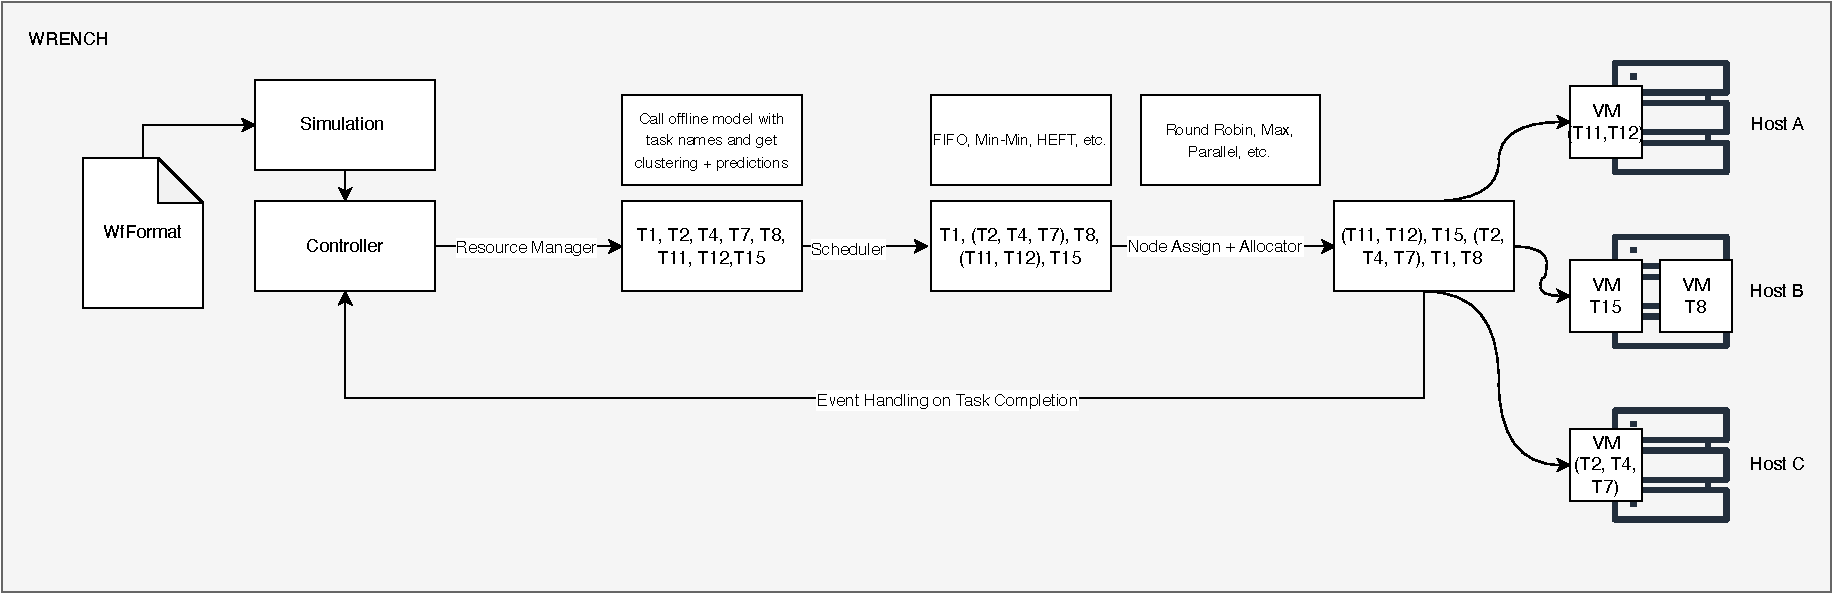
\includegraphics[scale=0.45]{fig/04/04-coloc-problem.pdf}
    \small
    \caption{Coloc Problem}
    \label{fig:04-coloc-problem}
    \tiny
    Das ist eine Beschreibung der Abbildung.
\end{figure}

Since our goal is to map not individual tasks but clusters of tasks, we embed the retrieval of co-location information derived from \textit{ShaReComp} directly into this stage of the scheduling process. In the illustrated example, the co-location hints result in consolidated groups such as T1, (T2, T4, T7), T8, (T11, T12), and T15. After clustering, the next step is to determine which compute host can best accommodate each task group. To this end, we define an interface for node assignment strategies that can either prioritize hosts with the most idle compute cores or distribute task clusters evenly across all available nodes to ensure balanced utilization. Finally, the allocation component creates virtual machines for each task cluster and launches them on their designated hosts, completing the mapping and allocation workflow. Through this exemplified design, we establish a foundation that not only enables the embedding and study of the co-location problem within an execution environment but also allows for systematic comparison through modular component interfaces. The following section formally introduces the simulation environment and the system model that represents our algorithmic formulation of the co-location problem.

% System Model that was used for the heuristic design.
\myparagraph{Simulation System Model}

\textbf{Workflow Properties}

Let the workflow be represented as a directed acyclic graph (DAG)
\[
    G = (T, E)
\]
where
\begin{itemize}
    \item $T = \{t_1, t_2, \dots, t_n\}$ denotes the set of \textbf{tasks}, and
    \item $E \subseteq T \times T$ denotes \textbf{data or control dependencies} between tasks.
\end{itemize}
A directed edge $(t_i, t_j) \in E$ indicates that task $t_j$ can start only after $t_i$ has completed.

\textbf{Task Properties}

Each task \( t_i \in T \) is associated with the following attributes:
\[
    \begin{array}{rcll}
        \text{req\_cores}(t_i) & \in & \mathbb{N}_{\ge 1} & \text{number of CPU cores required}, \\[4pt]
        \text{req\_mem}(t_i)   & \in & \mathbb{R}_{>0}    & \text{memory requirement in bytes.}
    \end{array}
\]

\textbf{Infrastructure Model}

Let \( \mathcal{H} = \{h_1, h_2, \dots, h_m\} \) denote the set of available \textbf{hosts},
where each host \( h_j \) is characterized by
\[
    C_j \in \mathbb{N}_{>0} \text{ (total number of cores)}, \qquad
    c(h_j) \in \mathbb{N}_{\ge 0} \text{ (current number of idle cores).}
\]

A \textbf{virtual machine (VM)} is represented as
\[
    v = (C_v, M_v, h_j),
\]
where \( C_v \) is the number of virtual cores, \( M_v \) the assigned memory,
and \( h_j \) the physical host on which it is instantiated.

The set of currently \textbf{ready tasks} (those whose dependencies are satisfied) is denoted by
\[
    \mathcal{Q} = \{t_1, t_2, \dots, t_k\}.
\]

\textbf{Resource Assignment}

A mapping of tasks to hosts and VMs is represented as
\[
    M = (h, \mathcal{T}_h, \text{colocMap}_h, \Phi_h),
\]
where
\begin{itemize}
    \item $h \in \mathcal{H}$ is the assigned host,
    \item $\mathcal{T}_h \subseteq T$ is the set of tasks mapped to $h$,
    \item $\text{colocMap}_h$ describes task clusters on $h$, and
    \item $\Phi_h$ represents associated file or data locations.
\end{itemize}
The set of mappings for an allocation interval is written as
\[
    \mathcal{M} = \{ M_1, M_2, \dots, M_p \}.
\]

\textbf{Task Co-location}

A \textbf{co-location mapping}, produced by a scheduler is defined as
\[
    \text{colocMap} = \{ (C_i, \mathcal{C}_i) \mid \mathcal{C}_i \subseteq T \},
\]
where $\mathcal{C}_i$ is a \textbf{cluster of tasks} to be executed together within a single virtual machine, ideally selected based on their resource affinity or complementary utilization patterns.

\textbf{Oversubscription}

An \textbf{oversubscription factor} $\alpha \in [0,1]$ allows up to
\[
    N_{\max}(h_j) = \lceil C_j (1 + \alpha) \rceil
\]
tasks to be scheduled concurrently on a VM on host $h_j$.


\textbf{Execution Dynamics}

At runtime:
\begin{itemize}
    \item \textbf{Node Assigners} determine host placement.
    \item \textbf{Schedulers} generate task queues and co-location groupings.
    \item \textbf{Allocators} instantiate and start VMs according to host-task mappings.
    \item The \textbf{Job Manager} executes tasks, monitors VM lifecycles, and updates resource states.
\end{itemize}

We present the unified algorithm that governs the overall behavior of our simulation framework. This algorithm formalizes how workflow tasks are scheduled, assigned, and executed under different resource management strategies, including optional co-location support through \textit{ShaReComp}.

% Blueprint Algorithm 
\begin{algorithm}[H]
    \caption{ShaReComp Simulation - WRENCH Framework}
    \label{alg:sharecomp_unified}
    \KwIn{workflow \( G=(T,E) \), hosts \( \mathcal{H}=\{h_1,\dots,h_m\} \), scheduling policy \( \pi \), oversubscription factor \( \alpha \), optional co-location API \( \mathcal{S} \)}
    \KwOut{workflow executed with policy-driven scheduling, node assignment, and adaptive resource management}

    \BlankLine
    Initialize system state: host capacities, ready queue \( \mathcal{Q} \), and monitoring layer\\

    \While{workflow \( G \) not completed}{
        Update \( \mathcal{Q} \) with all newly ready tasks\\
        Perform \textbf{task scheduling}: prioritize tasks in \( \mathcal{Q} \) according to policy \( \pi \)\\
        Perform \textbf{node assignment}: select suitable host(s) \( h \in \mathcal{H} \) using \( \pi \)\\
        Perform \textbf{resource allocation}: determine allowed capacity \( n_{\max}=f(c(h),\alpha) \) and reserve resources\\
        \If{policy \( \pi \) supports co-location}{
            Optionally query \( \mathcal{S} \) to group tasks by affinity and launch them on shared VMs
        }\Else{
            Launch one task per VM on assigned host
        }
        Monitor execution and task completions\\
        Release resources and enqueue successors of completed tasks
    }
    \Return{workflow complete}
\end{algorithm}

To evaluate the effectiveness of the \textit{ShaReComp} approach, we define several scheduling and node assignment algorithms that differ in their treatment of resource sharing and task placement. All of these algorithms build upon the unified simulation blueprint presented in \ref{alg:sharecomp_unified} and serve as comparative baselines. The first category of baselines executes each task in its own virtual machine, thereby avoiding any form of co-location. The second category enables task co-location by grouping multiple tasks within shared virtual machines and applying different host prioritization and allocation strategies. A third category extends this idea through controlled oversubscription, where more tasks are assigned to a virtual machine than the available reserved resources allow, deliberately inducing resource contention to test system robustness. Detailed algorithmic definitions are provided in the appendix, while \ref{cha:evaluation} discusses their comparative behavior in depth. The \textit{ShaRiff} algorithms build directly on top of these baselines, extending them with co-location awareness derived from \textit{ShaReComp}. In doing so, they replace random or static task grouping with data-driven consolidation decisions that account for resource affinity and contention characteristics.

\myparagraph{Algorithmic Examples of Task Mapping with guided Co-location}
\label{sec:co-location_strategies}

This section concludes our approach by introducing the main contribution of this thesis: the integration of the \textit{ShaReComp} methodology into the workflow execution process. To this end, we design four scheduling algorithms collectively referred to as \textit{ShaRiff} (Share Resources if Feasible). Each \textit{ShaRiff} variant implements a distinct strategy for mapping consolidated task clusters onto available compute hosts, while the co-location decisions themselves are consistently guided by the \textit{ShaReComp} approach introduced in Section \ref{sec:task_clustering}. An overview of the four \textit{ShaRiff} variants and their respective strategies is provided in Table \ref{tab:shariff_overview}.

% Table with \textit{ShaRiff} Overview stuff.
\begin{table}[H]
    \centering
    \footnotesize
    \begin{tabularx}{\textwidth}{l p{10cm}}
        \toprule
        \textbf{Algorithm}      & \textbf{Type}                                                                                                  \\
        \midrule
        \textit{ShaRiff} 1      & Biggest Host first, parallel Host-backfilling and mapping of Task Clusters                                     \\
        \textit{ShaRiff} 2      & Biggest Host first, parallel Host-backfilling and mapping of Task Clusters with controlled VM Oversubscription \\
        \textit{ShaRiff} 3      & Round-Robin Assignment of Task Clusters, No parallelism                                                        \\
        \textit{ShaRiff} MinMin & Biggest Host first, parallel Host-backfilling and mapping of ordered Task Clusters                             \\
        \bottomrule
    \end{tabularx}
    \small
    \caption{Overview of the \textit{ShaRiff} scheduling variants that make use of ShaReComp.}
    \label{tab:shariff_overview}
\end{table}


In the following, we provide a detailed description of the behavior of each \textit{ShaRiff} algorithm, followed by its formal algorithmic representation.

% \textit{ShaRiff} 1
% Algorithm
\begin{algorithm}[H]
    \caption{ShaRiff 1 — Biggest Host first, parallel Host-backfilling and mapping of Task Clusters}
    \label{alg:sharecomp}
    \KwIn{workflow \( G=(T,E) \), hosts \( \mathcal{H}=\{h_1,\dots,h_m\} \), idle cores \( c(h_j) \), ShaReComp co-location API \( \mathcal{S} \)}
    \KwOut{all tasks \( t_i\in T \) executed with contention-aware co-location for improved efficiency and utilization}

    \BlankLine
    Initialize idle cores \( c(h_j)\gets C_j \) for all \( h_j\in\mathcal{H} \);
    Initialize ready queue \( \mathcal{Q} \) with all source tasks of \( G \) (FIFO order)

    \BlankLine
    \While{not all tasks \( t_i\in T \) completed}{
        \If{\( \mathcal{Q} \) is empty}{
            Wait until any task \( t_r \) completes;
            Release its cores: \( c(h(t_r)) \gets c(h(t_r)) + \text{req\_cores}(t_r) \);
            For each successor \( t_s \) of \( t_r \), enqueue \( t_s \) into \( \mathcal{Q} \) if all predecessors are completed;
            \textbf{continue}
        }

        Build available-host list \( L=\{\,h\in\mathcal{H}\mid c(h)>0\,\} \), sorted by \( c(h) \) descending;
        Initialize empty host task mapping list \( \mathcal{M} \);

        \BlankLine
        \ForEach{host \( h\in L \) and while \( \mathcal{Q} \) not empty}{
            Select up to \( c(h) \) ready tasks from \( \mathcal{Q} \) into \( \mathcal{T}_h \);
            Compute file-location map \( \Phi(\mathcal{T}_h) \);
            Query ShaReComp API: \( \text{colocMap} \gets \mathcal{S}(\mathcal{T}_h) \) \tcp*[r]{returns co-location groups}
            Add mapping \( (h,\mathcal{T}_h,\Phi(\mathcal{T}_h),\text{colocMap}) \) to \( \mathcal{M} \);
        }

        \BlankLine
        \ForEach{mapping \( (h,\mathcal{T}_h,\Phi,\text{colocMap}) \in \mathcal{M} \)}{
            \ForEach{group \( \mathcal{C}_k \in \text{colocMap} \)}{
                \( C_{\text{req}} \gets \text{sum(req\_cores}(\mathcal{C}_k)) \);
                \( M_{\text{req}} \gets \text{sum(req\_mem}(\mathcal{C}_k)) \);
                Allocate \( v_h = (C_{\text{req}}, M_{\text{req}}, h) \);
                Launch all \( t \in \mathcal{C}_k \) on \( v_h \);
                \( c(h) \gets \max(0, c(h) - C_{\text{req}}) \);
                Remove \( \mathcal{C}_k \) from \( \mathcal{Q} \);
            }
        }

        \BlankLine
        Wait until any task \( t_r \) completes;
        Release its cores: \( c(h(t_r)) \gets c(h(t_r)) + \text{req\_cores}(t_r) \);
        \If{no active tasks remain on its VM}{ Destroy VM }
        For each successor \( t_s \) of \( t_r \): if all predecessors are completed, enqueue \( t_s \) into \( \mathcal{Q} \);
    }
    \Return{workflow complete}

\end{algorithm}

This variant implements \textit{ShaRiff} 1, which augments a FIFO pipeline with the external co-location adviser \textit{ShaReComp} and a cluster-aware allocator. Tasks are dequeued in strict arrival order. Before placement, the scheduler invokes \textit{ShaReComp} with the current set of ready tasks and receives clusters of jobs that are computed to co-locate well. The node-assignment stage then ranks hosts by descending idle-core capacity and fills the largest host first. It forms a batch of up to that hosts idle cores and attaches the \textit{ShaRiff} cluster map to the batch. If tasks remain, it proceeds to the next host in the ranked list. A small queue path ensures dispatch even when only a few tasks are available.
The allocator realizes the advisers plan one VM per recommended cluster on the chosen host. For each multi-task cluster, it provisions a VM whose vCPU count and memory equal the sum of the clustered tasks declared requirements, starts the VM, and submits the tasks to that same virtual compute service. Singleton clusters are grouped into a shared VM on the host to avoid VM fragmentation.
Conceptually, \textit{ShaRiff} preserves FIFO ordering and capacity-ranked host filling, but replaces random batching with adviser-driven clustering.

% \textit{ShaRiff} 2
% Algorithm
\begin{algorithm}[H]
    \caption{ShaRiff 2 — Biggest Host first, parallel Host-backfilling and mapping of Task Clusters with controlled VM Oversubscription}
    \label{alg:sharecomp_oversub}
    \KwIn{workflow \( G=(T,E) \), hosts \( \mathcal{H}=\{h_1,\dots,h_m\} \), idle cores \( c(h_j) \), oversubscription factor \( \alpha \), ShaReComp co-location API \( \mathcal{S} \)}
    \KwOut{workflow executed with affinity-based co-location, maximal host parallelism, and safe oversubscription}

    \BlankLine
    Initialize idle cores \( c(h_j)\gets C_j \) for all \( h_j\in\mathcal{H} \)
    Initialize ready queue \( \mathcal{Q} \) with all source tasks of \( G \) (FIFO order)

    \BlankLine
    \While{not all tasks \( t_i\in T \) completed}{
        \If{\( \mathcal{Q} \) is empty}{
            Wait until any task \( t_r \) completes
            Release its cores: \( c(h(t_r)) \gets c(h(t_r)) + \text{req\_cores}(t_r) \)
            For each successor \( t_s \) of \( t_r \), enqueue \( t_s \) into \( \mathcal{Q} \) if all predecessors are completed\\
            \textbf{continue}
        }

        Build available-host list \( L=\{\,h\in\mathcal{H}\mid c(h)>0\,\} \), sorted by \( c(h) \) descending
        Initialize empty host task mapping list \( \mathcal{M} \)

        \BlankLine
        \ForEach{host \( h\in L \) and while \( \mathcal{Q} \) not empty}{
            Compute oversubscription limit \( n_{\max} = \lceil c(h) \times (1 + \alpha) \rceil \)
            Select up to \( n_{\max} \) ready tasks from \( \mathcal{Q} \) into \( \mathcal{T}_h \)
            Compute file-location map \( \Phi(\mathcal{T}_h) \)
            Query ShaReComp API: \( \text{colocMap} \gets \mathcal{S}(\mathcal{T}_h) \) \tcp*[r]{returns co-location groups}
            Add mapping \( (h,\mathcal{T}_h,\Phi(\mathcal{T}_h),\text{colocMap}) \) to \( \mathcal{M} \)
        }

        \BlankLine
        \ForEach{mapping \( (h,\mathcal{T}_h,\Phi,\text{colocMap}) \in \mathcal{M} \)}{
            \ForEach{group \( \mathcal{C}_k \in \text{colocMap} \)}{
                \( C_{\text{req}} \gets \text{sum(req\_cores}(\mathcal{C}_k)) \)
                \( M_{\text{req}} \gets \text{sum(req\_mem}(\mathcal{C}_k)) \)
                \If{\( C_{\text{req}} > c(h) \)}{
                    Allocate \( v_h = (c(h), M_{\text{req}}, h) \); \tcp*[r]{oversubscription active}
                }
                \Else{
                    Allocate \( v_h = (C_{\text{req}}, M_{\text{req}}, h) \)
                }
                Launch all \( t \in \mathcal{C}_k \) on \( v_h \)
                \( c(h) \gets \max(0, c(h) - C_{\text{req}}) \)
                Remove \( \mathcal{C}_k \) from \( \mathcal{Q} \)
            }
        }

        \BlankLine
        Wait until any task \( t_r \) completes
        Release its cores: \( c(h(t_r)) \gets c(h(t_r)) + \text{req\_cores}(t_r) \)
        \If{no active tasks remain on its VM}{ Destroy VM }
        For each successor \( t_s \) of \( t_r \): if all predecessors are completed, enqueue \( t_s \) into \( \mathcal{Q} \)
    }
    \Return{workflow complete}
\end{algorithm}

% \textit{ShaRiff} 2
This variant extends \textit{ShaRiff} 1 by controlled oversubscription during placement and VM sizing. Tasks are dequeued in arrival order. Before dispatch, the scheduler queries ShaReComp with the current ready set and receives clusters of tasks pcomputed to co-locate well. Hosts are ranked by descending idle-core capacity; the assigner then fills the largest host first with a batch whose size may exceed the hosts free cores by a fixed factor of in our example 25\%. If tasks remain, it proceeds to the next host and repeats.
The allocator implements the advisers plan one VM per cluster on the chosen host, but with oversubscription semantics. For multi-task clusters, it provisions a VM whose vCPU and memory equal the sum of the clusters requests—even if that exceeds the hosts currently free cores. For single task clusters collected on the same host, it provisions a shared VM and caps vCPUs at the hosts free cores when necessary.
Because ShaReComp groups complementary tasks, oversubscription holds the potential to translate into higher throughput and energy efficiency. However, when clustered tasks are less complementary, contention can surface, making this variant an explicit trade-off between utilization and interference.

% \textit{ShaRiff} 3
% Algorithm

\begin{algorithm}[H]
    \caption{ShaRiff 3 — Round-Robin Assignment of Task Clusters, No parallelism}
    \label{alg:sharecomp_rr}
    \KwIn{workflow \( G=(T,E) \), hosts \( \mathcal{H}=\{h_1,\dots,h_m\} \), idle cores \( c(h_j) \), ShaReComp co-location API \( \mathcal{S} \)}
    \KwOut{tasks executed using round-robin host selection with affinity-based VM co-location}

    \BlankLine
    Initialize idle cores \( c(h_j)\gets C_j \) for all \( h_j\in\mathcal{H} \)
    Initialize ready queue \( \mathcal{Q} \) with all source tasks of \( G \) (FIFO order)
    Initialize round-robin index \( r \gets 0 \)

    \BlankLine
    \While{not all tasks \( t_i\in T \) completed}{
        \If{\( \mathcal{Q} \) is empty}{
            Wait until any task \( t_r \) completes
            Release its cores: \( c(h(t_r)) \gets c(h(t_r)) + \text{req\_cores}(t_r) \)
            For each successor \( t_s \) of \( t_r \), enqueue \( t_s \) into \( \mathcal{Q} \) if all predecessors are completed\\
            \textbf{continue}
        }

        Select next host \( h = \mathcal{H}[r \bmod |\mathcal{H}|] \)
        Update round-robin index: \( r \gets (r + 1) \bmod |\mathcal{H}| \)
        Retrieve available cores \( C = c(h) \)
        Select up to \( C \) ready tasks from \( \mathcal{Q} \) into \( \mathcal{T}_h \)
        Query ShaReComp API: \( \text{colocMap} \gets \mathcal{S}(\mathcal{T}_h) \) \tcp*[r]{returns co-location groups}

        \BlankLine
        \ForEach{group \( \mathcal{C}_k \in \text{colocMap} \)}{
            \( C_{\text{req}} \gets \text{sum(req\_cores}(\mathcal{C}_k)) \)
            \( M_{\text{req}} \gets \text{sum(req\_mem}(\mathcal{C}_k)) \)
            Allocate \( v_h = (C_{\text{req}}, M_{\text{req}}, h) \)
            Launch all \( t \in \mathcal{C}_k \) on \( v_h \)
            \( c(h) \gets \max(0, c(h) - C_{\text{req}}) \)
            Remove \( \mathcal{C}_k \) from \( \mathcal{Q} \)
        }

        \BlankLine
        Wait until any task \( t_r \) completes
        Release its cores: \( c(h(t_r)) \gets c(h(t_r)) + \text{req\_cores}(t_r) \)
        \If{no active tasks remain on its VM}{ Destroy VM }
        For each successor \( t_s \) of \( t_r \): if all predecessors are completed, enqueue \( t_s \) into \( \mathcal{Q} \)
    }
    \Return{workflow complete}
\end{algorithm}

\textit{ShaRiff} 3 combines round-robin first-fit placement with \textit{ShaReComp}-guided intra-VM co-location. The scheduler releases tasks strictly in arrival order. The node-assignment component scans hosts in round-robin fashion and picks the first host reporting at least one idle core. It then pulls up to that hosts idle-core capacity worth of ready tasks and queries \textit{ShaReComp} for a co-location plan over this batch.
The allocator realizes \textit{ShaReComp's} plan one VM per suggested cluster on the chosen host. For each multi-task cluster, it sizes the VM by summing vCPU and memory requirements of the clusters tasks, starts the VM, and submits all cluster tasks to the same virtual compute service.
Conceptually, the policy is first-fit host, adviser-driven packing. Unlike the other variants, this strategy does not oversubscribe cores. It fills only the currently free capacity of the first eligible host and relies on \textit{ShaReComp's} clustering to raise utilization and efficiency through informed co-location.

% MinMin extension
This scheduler variant extends the \textit{ShaRiff} framework with a MinMin ordering layer, a classical heuristic from list scheduling. Instead of operating on individual tasks, it applies the MinMin principle to task clusters generated by \textit{ShaReComp's} co-location analysis. At each scheduling interval, the scheduler requests a new clustering of ready tasks, queries the prediction service using the models introduced in \ref{sec:prediciton_kcca_rfr} with \ref{alg:sharecomp_prediction} for estimated runtimes, and orders clusters in ascending order of predicted execution time. The \textit{ShaRiff} node assignment and VM allocator then manage placement and resource provisioning. In essence, this forms a MinMin scheduler over co-located clusters, combining \textit{ShaRiff's} affinity-based co-location with prediction-guided execution ordering to minimize queueing delays and improve overall workflow completion time.

% ShaRiff 1 - MinMin
\begin{algorithm}[H]
    \caption{ShaRiff 1 MinMin — Biggest Host first, parallel Host-backfilling and ordered mapping of Task Clusters}
    \label{alg:shariff_minmin}
    \KwIn{workflow \( G=(T,E) \), hosts \( \mathcal{H}=\{h_1,\dots,h_m\} \), idle cores \( c(h_j) \), ShaReComp co-location API \( \mathcal{S} \), prediction service \( \mathcal{P} \)}
    \KwOut{all tasks \( t_i\in T \) executed with predictive ordering and contention-aware co-location}

    \BlankLine
    Initialize idle cores \( c(h_j)\gets C_j \) for all \( h_j\in\mathcal{H} \)
    Initialize ready queue \( \mathcal{Q} \) with all source tasks of \( G \) (FIFO order)

    \BlankLine
    \While{not all tasks \( t_i\in T \) completed}{
        \If{\( \mathcal{Q} \) is empty}{
            Wait until any task \( t_r \) completes\\
            Release its cores: \( c(h(t_r)) \gets c(h(t_r)) + \text{req\_cores}(t_r) \)
            For each successor \( t_s \) of \( t_r \), enqueue \( t_s \) into \( \mathcal{Q} \) if all predecessors are completed\\
            \textbf{continue}
        }

        Build available-host list \( L=\{\,h\in\mathcal{H}\mid c(h)>0\,\} \), sorted by \( c(h) \) descending
        Initialize empty host-task mapping list \( \mathcal{M} \)

        \BlankLine
        \ForEach{host \( h\in L \) and while \( \mathcal{Q} \) not empty}{
            Select up to \( c(h) \) ready tasks from \( \mathcal{Q} \) into \( \mathcal{T}_h \)
            Compute file-location map \( \Phi(\mathcal{T}_h) \)\\
            Query ShaReComp API: \( \text{colocMap} \gets \mathcal{S}(\mathcal{T}_h) \) \tcp*[r]{returns co-location groups}
            Add mapping \( (h,\mathcal{T}_h,\Phi(\mathcal{T}_h),\text{colocMap}) \) to \( \mathcal{M} \)
        }

        \BlankLine
        \tcp{Predictive MinMin ordering based on estimated runtimes}
        Query prediction API: \( \text{predictions} \gets \mathcal{P}(\mathcal{M}) \)
        Sort mappings \( \mathcal{M} \) by ascending predicted runtime: \( \mathcal{M}_{sorted} = \text{sort}_{asc}(\mathcal{M}, \text{key}=r_i) \)

        \BlankLine
        \ForEach{mapping \( (h,\mathcal{T}_h,\Phi,\text{colocMap}) \in \mathcal{M}_{sorted} \)}{
            \ForEach{group \( \mathcal{C}_k \in \text{colocMap} \)}{
                \( C_{\text{req}} \gets \text{sum(req\_cores}(\mathcal{C}_k)) \)
                \( M_{\text{req}} \gets \text{sum(req\_mem}(\mathcal{C}_k)) \)
                Allocate \( v_h = (C_{\text{req}}, M_{\text{req}}, h) \)
                Launch all \( t \in \mathcal{C}_k \) on \( v_h \)
                \( c(h) \gets \max(0, c(h) - C_{\text{req}}) \)
                Remove \( \mathcal{C}_k \) from \( \mathcal{Q} \)
            }
        }

        \BlankLine
        Wait until any task \( t_r \) completes\\
        Release its cores: \( c(h(t_r)) \gets c(h(t_r)) + \text{req\_cores}(t_r) \)
        \If{no active tasks remain on its VM}{ Destroy VM }
        For each successor \( t_s \) of \( t_r \): if all predecessors are completed, enqueue \( t_s \) into \( \mathcal{Q} \)
    }
    \Return{workflow complete}
\end{algorithm}
\clearpage
\section{Implementation}
\label{cha:implementation}
% TODO: Insert previous chapter references
This chapter details the technical implementation of the concepts introduced in the previous section. While the Approach chapter established the conceptual and algorithmic foundations of the proposed scheduling framework, the following sections focus on how these ideas were realized in practice. The implementation emphasizes architectural modularity, clear component interfaces, and the integration of machine learning-based decision layers within a simulation-driven environment. Each subsystem—from the monitoring client and statistical modeling backend to the simulation environment—was designed to remain functionally independent while communicating through well-defined data and control flows. This decoupled design not only facilitates reproducibility and maintainability but also enables future extensions, such as the replacement of predictive models or the addition of new scheduling policies, without major structural changes. The remainder of this chapter outlines the overall system architecture, mentions the chosen technologies and design principles, and describes the concrete implementation of the monitoring client, the statistical learning components, and the simulator setup.

\subsection{System Architecture}
\label{sec:system_architecture}
% Overview sketch

\subsection{Technology and Design Choices}
\label{sec:technology_and_design_choices}
% Provide a table per number of the previous figure with the technology and design choice and a brief justification.

\begin{table}[H]
    \centering
    \caption{Monitoring features and associated technical components.}
    \label{tab:monitoring_layers}
    \renewcommand{\arraystretch}{1.15}
    \resizebox{\textwidth}{!}{
        \begin{tabular}{
            p{4.5cm}
            >{\centering\arraybackslash}p{2.8cm}
            p{8.2cm}
            }
            \toprule
            \textbf{Component Category} & \textbf{Software Used}                                   & \textbf{Comments / Functionality}                               \\
            \midrule

            \multicolumn{3}{l}{\textbf{Workflow Execution}}                                                                                                          \\[3pt]
            Operating System            & Ubuntu 22.04.5 LTS                                       & Base system environment for all components.                     \\
            Kernel                      & Linux 5.15.0-143-generic                                 & Provides low-level system resource management.                  \\
            Workflow Management Engine  & Nextflow 25.06.0                                         & Controls workflow DAG execution and task dependency resolution. \\
            Virtualization Layer        & Docker Engine 28.3.1 (Community)                         & Provides isolated VM environments for task execution.           \\
            Resource Manager            & Slurm 24.05.2                                            & Allocates CPU and memory resources dynamically across hosts.    \\

            \midrule
            \multicolumn{3}{l}{\textbf{Monitoring System}}                                                                                                           \\[3pt]
            Time-Series Database        & Prometheus Server 3.3.1                                  & Central metric collector and time-series database.              \\
            Monitoring Client           & Go 1.24.1                                                & Collects per-node and per-container resource metrics.           \\

            \midrule
            \multicolumn{3}{l}{\textbf{Workload Experiments}}                                                                                                        \\[3pt]
            Benchmark Execution         & stress-ng 0.13.12                                        & Generates controlled CPU, memory, and I/O workloads.            \\
            Monitoring                  & Deep-Mon (custom fork) with Python 3.10.12 \& BCC 0.35.0 & Captures resource traces during workload execution.             \\

            \midrule
            \multicolumn{3}{l}{\textbf{Data Analysis}}                                                                                                               \\[3pt]
            Feature Engineering         & Jupyter Kernel 6.29.5, Python 3.10.12, Poetry 2.1.2      & Derives and normalizes temporal task signatures.                \\
            Clustering                  & scikit-learn 1.5.2                                       & Groups similar task behaviors into consolidated classes.        \\
            KCCA                        & CCA-Zoo 2.5.0                                            & Learns correlations between performance and energy domains.     \\
            Random Forest Regressor     & scikit-learn 1.5.2                                       & Predicts runtime and power consumption from task signatures.    \\
            Kernel Ridge Regression     & scikit-learn 1.5.2                                       & Baseline model for non-linear regression comparison.            \\

            \midrule
            \multicolumn{3}{l}{\textbf{Simulation Framework}}                                                                                                        \\[3pt]
            Workflow Tracing            & Nextflow Tracer (custom fork)                            & Records execution-level metadata for simulation replay.         \\
            Simulation Engine           & WRENCH 2.7 \& C++17                                      & Evaluates scheduling strategies under controlled conditions.    \\
            Clustering API              & FastAPI 0.1.0, Python 3.10.12                            & Provides task grouping via ShaReComp integration.               \\
            Prediction API              & FastAPI 0.1.0, Python 3.10.12                            & Interfaces learned models for runtime and energy estimation.    \\

            \bottomrule
        \end{tabular}
    }
\end{table}


\subsection{Decoupled Design for further Research}
\label{sec:extensibility_through_decoupled_design}
The extensibility of the overall system is achieved through a decoupled design that separates monitoring, modeling, and simulation components while maintaining clear communication interfaces between them. Each part of the system can evolve independently without impacting others, enabling modular experimentation with new data sources, predictive models, or scheduling strategies. This modularity supports reproducibility and future extensibility, as new data collection layers or simulation backends can be added by extending interfaces rather than rewriting existing code.

\subsubsection{Configurable Monitoring Client}
\label{sec:monitoring_client}
The monitoring client exemplifies this philosophy by relying on a flexible configuration-driven architecture. Using a YAML-based configuration file, it dynamically defines which metrics to collect from heterogeneous data sources such as Prometheus exporters, cAdvisor, eBPF probes, or SNMP-based sensors. The configuration specifies not only the metric names and queries but also the identifiers and units, allowing seamless adaptation to different environments or workflow engines. This separation of logic and configuration enables the same client to operate across diverse infrastructures without recompilation. The clients implementation, built on the Prometheus API, abstracts away the complexity of time-range queries and concurrent metric fetching through lightweight threading and synchronization mechanisms. As a result, developers can extend the monitoring framework simply by adding new data sources or metrics to the configuration file, without altering the underlying collection logic.

% Table to show the config file of the monitoring client

\begin{table}[H]
    \centering
    \caption{Adaptable Monitoring Configuration Overview.}
    \label{tab:monitoring_config_overview}
    \renewcommand{\arraystretch}{1.15}
    \resizebox{\textwidth}{!}{
        \begin{tabular}{
            p{3.5cm}
            >{\centering\arraybackslash}p{2cm}
            p{5cm}
            p{6cm}
            }
            \toprule
            \textbf{Monitoring Target} & \textbf{Enabled} & \textbf{Supported Data Sources}                         & \textbf{Collected Metric Types / Adaptability Notes}                                                                    \\
            \midrule

            Task Metadata              &                  & slurm-job-exporter                                      & Collects job metadata (state, runtime, working directory). Can adapt to other job schedulers.                           \\

            CPU                        &                  & cAdvisor, ebpf-mon, docker-activity                     & Captures CPU time and cycles from both container and kernel levels. Supports switching sources for varying granularity. \\

            Memory                     &                  & cAdvisor, docker-activity                               & Tracks memory utilization at container or process level. Configurable for byte- or percentage-based metrics.            \\

            Disk                       &                  & cAdvisor                                                & Monitors block I/O and filesystem throughput. Supports extension with storage exporters.                                \\

            Network                    &                  & cAdvisor (optional)                                     & Disabled by default due to noise. Can be enabled for network-intensive workflows.                                       \\

            Energy                     &                  & docker-activity, ebpf-mon, ipmi-exporter, snmp-exporter & Multi-layer energy monitoring from container to node level. Adaptable to hardware sensors and external power meters.    \\

            \midrule
            \multicolumn{4}{l}{\textbf{Prometheus Configuration}}                                                                                                                                                                             \\[3pt]
            \multicolumn{4}{p{16.5cm}}{
                The Prometheus backend collects all metrics via configurable scrape intervals and targets. Controller and worker nodes can be flexibly defined, enabling distributed monitoring setups.
            }                                                                                                                                                                                                                                 \\

            \bottomrule
        \end{tabular}
    }
\end{table}

\subsubsection{Enabling Access to Co-location Hints in the Simulator}
\label{sec:statistical_modeling}
The statistical modeling component, implemented as a standalone FastAPI service, follows a similar modular design. It exposes a clean, language-agnostic HTTP API that separates the inference logic from data ingestion and model management. The service maintains state for clustering and prediction requests, delegating core computational tasks to dedicated helper functions. This decoupling makes it straightforward to replace or add new predictive models, such as neural architectures or alternative regression approaches, without modifying the API contract. The clustering and prediction endpoints can interact with any external workflow manager or simulator via standardized JSON payloads, ensuring flexibility in integrating new pipelines or retraining procedures. This independence between model serving and data processing pipelines also simplifies scalability, allowing the modeling service to be containerized and deployed independently for distributed or cloud-based setups.

% Graphic with API Endpoints showing the implemented capabilities:

\begin{table}[H]
    \centering
    \caption{Overview of REST API Endpoints Exposed by the ShaReComp Service.}
    \label{tab:api_endpoints}
    \renewcommand{\arraystretch}{1.15}
    \resizebox{\textwidth}{!}{
        \begin{tabular}{
            p{0.8cm}
            p{5.3cm}
            >{\centering\arraybackslash}p{2cm}
            p{9cm}
            }
            \toprule
            \textbf{\#} & \textbf{Endpoint}               & \textbf{Method} & \textbf{Description / Response Schema}                   \\
            \midrule

            1           & \texttt{/clusterize\_jobs}      & POST            &
            Clusters nf-core jobs based on historical data. \newline
            \textit{Request:} \texttt{ClusterizeJobsRequest} (list of job names). \newline
            \textit{Response:} \texttt{ClusterizeJobsResponse} (cluster mapping with run ID).                                          \\

            2           & \texttt{/predict}               & POST            &
            Predicts runtime and power consumption for consolidated job clusters. \newline
            \textit{Request:} \texttt{PredictRequest} (cluster IDs, model types). \newline
            \textit{Response:} \texttt{PredictionResponse} (predicted values for each model).                                          \\

            \midrule
            \multicolumn{4}{l}{\textbf{Component Schemas}}                                                                             \\[3pt]

            --          & \texttt{ClusterizeJobsRequest}  & Object          &
            \textbf{Fields:} \texttt{job\_names} (array of strings). Required.                                                         \\

            --          & \texttt{ClusterizeJobsResponse} & Object          &
            \textbf{Fields:} \texttt{run\_id} (string), \texttt{clusters} (map of arrays). Required.                                   \\

            --          & \texttt{PredictRequest}         & Object          &
            \textbf{Fields:} \texttt{cluster\_ids} (array), \texttt{prediction\_models} (array of \texttt{PredictionModel}). Required. \\

            --          & \texttt{PredictionModel}        & Object          &
            \textbf{Fields:} \texttt{model\_type} (array of strings). Required.                                                        \\

            --          & \texttt{PredictionResponse}     & Object          &
            \textbf{Fields:} \texttt{run\_id} (string), \texttt{predictions} (nested map of numeric values). Required.                 \\


            \bottomrule
        \end{tabular}
    }
\end{table}

\subsubsection{Used Simulator Components}
\label{sec:simulator_setup}
The simulator setup further demonstrates the benefits of this decoupled design. The resource management layer of the simulator exposes generic interfaces for allocators, schedulers, and node assigners, allowing any of them to be replaced or combined dynamically at runtime. This separation allows the same simulator to execute both baseline and experimental resource allocation strategies without modifying the controller logic. Through this design, the simulator can execute diverse workflow types by merely switching configuration parameters or class bindings. Moreover, the integration of energy and performance tracing through independent services ensures that extending the simulator with new measurement capabilities does not interfere with the scheduling or execution logic.

% Show cpp code of base directory
\lstinputlisting[
    language=C++,
    caption={WRENCH C++ Simulation File},
    label={lst:cpp_sim},
    basicstyle=\ttfamily\footnotesize,
    keywordstyle=\color{blue},
    commentstyle=\color{gray},
    stringstyle=\color{red},
    numbers=left,
    numberstyle=\tiny,
    stepnumber=1,
    numbersep=5pt,
    breaklines=true,
    frame=single
]{/home/nfomin3/dev/ThesisDocument/fig/05/05-wrench-sim.cpp}
\clearpage
\section{Evaluation}
\label{cha:evaluation}
This chapter presents the evaluation setup and results of the task co-location approach and developed scheduling algorithms for nine heterogeneous, real-world scientific workflows executed in a simulated environment.
\subsection{Evaluation Setup}
\label{sec:evaluation_setup}
First, this section articulates the evaluation setup used in the experiments.

\subsubsection{Infrastructure}
\label{sec:evaluation_infrastructure}
The experiments were conducted on a single-node system equipped with an AMD EPYC 8224P 24-core, 48-thread processor and 188 GB of RAM. The processor supported simultaneous multithreading and frequency boosting up to 2.55 GHz, with 64 MB of shared L3 cache and a single NUMA domain ensuring uniform memory access across all cores. Storage was provided by a 3.5 TB NVMe SSD, and the system ran a 64-bit Linux environment.
To collect accurate power usage data, the node was connected to a 12-way switched and outlet-metered PDU (Expert Power Control 8045 by GUDE), which provided per-outlet power measurements via a REST API.

\subsubsection{Workflows}
\label{sec:evaluation_workflows}
% TODO: Add correct values there
Nine real-world, openly available scientific workflows from the nf-core repository have been used to measure how the developed approach performs in realistic scenarios. Specifically, the following workflows have been tested:
% Table with different workflows and their characteristics
\begin{table}[H]
    \centering
    \caption{Overview of evaluated nf-core workflows.}
    \label{tab:workflow_overview}
    \renewcommand{\arraystretch}{1.15}
    \resizebox{\textwidth}{!}{
        \begin{tabular}{
            p{3.5cm}
            >{\centering\arraybackslash}p{3cm}
            >{\centering\arraybackslash}p{3cm}
            >{\centering\arraybackslash}p{3cm}
            >{\centering\arraybackslash}p{3cm}
            }
            \toprule
            \textbf{Workflow}     & \textbf{Number of Tasks} & \textbf{Input Files} & \textbf{Output Files} & \textbf{Data Profile}                                    \\
            \midrule
            \texttt{atacseq}      & 72                       & 24                   & 185                   & Bulk chromatin accessibility sequencing (ATAC-seq)       \\
            \texttt{chipseq}      & 68                       & 22                   & 172                   & Bulk chromatin immunoprecipitation sequencing (ChIP-seq) \\
            \texttt{rnaseq}       & 54                       & 18                   & 160                   & Bulk RNA-seq expression quantification                   \\
            \texttt{scnanoseq}    & 83                       & 25                   & 210                   & Single-cell nanopore RNA-seq                             \\
            \texttt{smrnaseq}     & 59                       & 20                   & 142                   & Small RNA sequencing (miRNA/siRNA profiling)             \\
            \texttt{pixelator}    & 44                       & 16                   & 125                   & Spatial transcriptomics pixel-based expression mapping   \\
            \texttt{methylseq}    & 65                       & 21                   & 170                   & Whole-genome or targeted DNA methylation sequencing      \\
            \texttt{viralrecon}   & 51                       & 19                   & 150                   & Viral genome assembly and variant analysis               \\
            \texttt{oncoanalyser} & 97                       & 28                   & 260                   & Comprehensive somatic cancer genome analysis             \\
            \bottomrule
        \end{tabular}
    }
\end{table}

\subsubsection{Monitoring Configuration}
\label{sec:evaluation_monitoring_configuration}
The execution of the workflows and the accompanying monitoring data collection have been performed in a high-throughput computing environment with the following monitoring metrics being collected:
% Table with different combinations
\begin{table}[H]
    \centering
    \caption{Adaptable Monitoring Configuration Overview.}
    \label{tab:monitoring_config_overview}
    \renewcommand{\arraystretch}{1.15}
    \resizebox{\textwidth}{!}{
        \begin{tabular}{
            p{3.5cm}
            >{\centering\arraybackslash}p{2cm}
            p{5cm}
            p{6cm}
            }
            \toprule
            \textbf{Monitoring Target} & \textbf{Enabled} & \textbf{Supported Data Sources} & \textbf{Collected Metric Types / Adaptability Notes} \\
            \midrule

            Task Metadata              &                  & nextflow                        & Metrics                                              \\

            CPU                        &                  & cAdvisor, Deep-Mon              & Metrics                                              \\

            Memory                     &                  & cAdvisor, Deep-Mon              & Metrics                                              \\

            Disk                       &                  & cAdvisor, Deep-Mon              & Metrics                                              \\

            Energy                     &                  & Deep-Mon                        & Metrics                                              \\

            \midrule
            \multicolumn{4}{l}{\textbf{Prometheus Configuration}}                                                                                  \\[3pt]
            \multicolumn{4}{p{16.5cm}}{
                The Prometheus backend collects all metrics via configurable scrape intervals and targets. Controller and worker nodes can be flexibly defined, enabling distributed monitoring setups.
            }                                                                                                                                      \\

            \bottomrule
        \end{tabular}
    }
\end{table}

\subsubsection{Implemented Models for Task Clustering and Prediction}
\label{sec:evaluation_statistical_learning_methods}
As described in Chapter \ref{cha:implementation}, the statistical models—including the clustering and prediction components—are provided through a FastAPI implementation, allowing external simulation engines to interact with them programmatically. At the same time, the core functionality of the API service is based on a Jupyter Notebook that contains all implementations and evaluations of our approach and were executed on the infrastructure described in Section \ref{sec:evaluation_infrastructure}.

\subsubsection{Simulation Setup}
\label{sec:evaluation_simulation}

\paragraph{Simulated Platform Configuration}
The infrastructure described in Section \ref{sec:evaluation_infrastructure} was replicated within the SimGrid simulation environment using its platform description tool, as shown in the following XML configuration. The hosts core performance was calibrated by executing stress-ng benchmarks to determine realistic CPU speeds, while network throughput was measured using sysbench. To determine power states (P-states), the GUDE power meter was used to record power consumption in both idle and active conditions under varying load profiles generated with stress-ng. This procedure ensured that the simulated environment accurately reflected the performance and energy characteristics of the physical test system.

% Platform XML file 
\lstinputlisting[
    language=XML,
    caption={Example XML Configuration File},
    label={lst:xml_config}
]{/home/nfomin3/dev/ThesisDocument/fig/06/siena_cluster.xml}

\paragraph{Baseline Scheduling Algorithms}

To evaluate the effectiveness of the proposed approach, we compare it against a series of progressively refined baseline algorithms that address the co-location problem with increasing complexity. These baselines range from simple scheduling heuristics to more advanced strategies that gradually incorporate awareness of co-location effects. The following table summarizes all baselines considered in this study. It is important to note that while some of them already involve concurrent execution of tasks, this represents uncontrolled co-location rather than informed or optimized placement. For clarity and conciseness, detailed algorithmic designs of these baselines are provided in the appendix, while this section focuses on describing their conceptual behavior.

% Overview table over all baselines
\begin{table}[H]
    \centering
    \footnotesize
    \begin{tabularx}{\textwidth}{l p{10cm}}
        \toprule
        \textbf{Algorithm} & \textbf{Type}                                                                                              \\
        \midrule
        Baseline 1         & FIFO Scheduling, Exclusive Round-Robin Host Assignment, Exclusive VM Allocation                            \\
        Baseline 2         & FIFO Scheduling, Exclusive Host-Backfilling, Exclusive VM Allocation                                       \\
        Baseline 3         & Round-Robin Assignment of Task Clusters, No parallelism                                                    \\
        Baseline 3.1       & Biggest Host first, Mapping of random Task Clusters                                                        \\
        Baseline 3.2       & Biggest Host first, parallel Host-backfilling and mapping of random Task Clusters                          \\
        Baseline 4         & Biggest Host first, Mapping of random Task Clusters with Oversubscription                                  \\
        Baseline 4.1       & Biggest Host first, parallel Host-backfilling and mapping of random Task Clusters with VM Oversubscription \\
        \bottomrule
    \end{tabularx}
    \small
    \caption{Overview of Baseline Scheduling Algorithms}
    \label{tab:baselines_overview}
\end{table}

% W/O Co-location
\myparagraph{Baselines without Co-location}
% Baseline 1
The baseline scheduling algorithm implements a simple, sequential execution model designed to simulate isolated task processing within a virtualized cluster. The scheduling process is divided into three abstract components that operate in a fixed order: task scheduling, node assignment, and resource allocation. The scheduler applies a FIFO policy, maintaining a queue of workflow tasks sorted by their readiness. Tasks are retrieved from this queue strictly in order of arrival, preserving dependency constraints and ensuring a fully deterministic execution sequence without reordering or prioritization.
Once a task is selected for execution, the node assignment component distributes it across available compute hosts using a round-robin policy. This mechanism cycles through hosts in sequence, ensuring an even and systematic distribution of tasks across the cluster. No host is assigned more than one active task at a time, enforcing exclusive execution and preventing contention for shared resources.
% Baseline 2
The next variant keeps the same FIFO scheduler and VM-based allocator as Baseline 1, but replaces exclusive node assignment with a greedy backfilling policy. Tasks are still dequeued strictly in arrival order by the FIFO scheduler. For each ready task, the node assignment component queries the cluster for the current number of idle cores per host and performs a first-fit scan: it selects the first host that reports at least one idle core, without requiring the host to be completely idle. The allocator then provisions a VM on the chosen host, binds the tasks inputs/outputs, submits the job to that VM, and on completion shuts the VM down and destroys it.
% With co-location
\myparagraph{Baselines with Co-location}
% Baseline 3
Baseline 3 does not differ in the scheduling behavior but replaces the standard allocator and node assignment with components that allow for co-location. When the node assignment component queries the cluster for idle-core availability, it again selects the first host with available cores. However, instead of launching one VM per task, all ready tasks that fit within the hosts idle-core capacity are grouped into a single batch. These tasks are then co-located inside one shared VM instance that is dimensioned according to the aggregate resource requirements of the batch—its vCPU count and memory size are computed as the sum of the respective task demands.
Conceptually, this baseline captures the behavior of intra VM co-location, where multiple independent tasks share the same virtual machine instead of being distributed across separate ones.
% Baseline 3.1
Baseline 3 is extended by 2 variants where the first one extends the node assignment component to query the cluster for idle-core availability and selects the host with the maximum amount of available cores. However, instead of launching one VM per task, all ready tasks that fit within the hosts idle-core capacity are grouped into a single batch. These tasks are then co-located inside one shared VM instance that is dimensioned according to the aggregate resource requirements of the batch with its vCPU count and memory size are computed as the sum of the respective task demands.
% Baseline 3.2
The second extension replaces the placement policy with a selection step for the host with maximum idle cores. At each dispatch, the node-assignment component queries the cluster for the current idle cores per host map and picks the host with the largest number of free cores. It then forms a batch by taking as many ready tasks from the FIFO head as the chosen host can accommodate. Compared to first-fit co-location, it tends to reduce residual fragmentation by packing work onto the most spacious node, while still honoring FIFO ordering and leaving task runtime/I/O handling unchanged.
% Baseline 4
Baseline 4 retains the same FIFO scheduler but introduces a node assignment and allocation policy focused on maximizing parallel host utilization. Upon each scheduling cycle, the node assignment component queries the cluster for the current number of idle cores per host, filters out fully occupied nodes, and ranks the remaining hosts in descending order of available cores. It then assigns tasks in batches, filling the host with the highest idle capacity first and grouping as many ready tasks as the hosts idle-core count allows. Once the first host is filled, the process continues with the next host until all tasks in the ready queue are mapped.
% Baseline 4.1
The last baseline extends the previous one by allowing controlled CPU over-subscription during co-location.
At each scheduling cycle, the node assignment component queries per-host idle cores, sorts hosts in descending idle capacity, and fills the largest host first. Unlike the non-oversubscribed version, the per-host batch may exceed the currently idle cores by a fixed factor the batch limit is set to. The procedure continues down the ranked host list, forming one batch per host in the same cycle.
The allocator provisions one VM per host batch, but caps the VMs vCPU count to the hosts actual idle cores at allocation time not the sum of task core demands, while sizing memory to the aggregate of the batched tasks. All tasks in the batch are then submitted to that single VM and execute concurrently on a vCPU pool intentionally smaller than their combined declared cores. The VM remains active until all co-located tasks complete, then it is shut down and destroyed.
Crucially, the degree of contention and realized speedup or slowdown depends on the complementarity of the co-located task profiles. When CPU-, memory-, and I/O-intensive phases overlap unfavorably oversubscription amplifies interference and queueing on scarce vCPUs. When profiles are complementary, the same oversubscription admits more useful overlap with less contention, improving per host throughput. Conceptually, this variant implements parallel, capacity-ranked random task co-location with controlled oversubscription.

\subsection{Experiment Results}
\label{sec:experiment_results}
The section on experimental results is organized as follows. We revisit the approach introduced in Chapter \ref{sec:measuring_resource_contention} by examining the workload experiments and the resulting measurements that form the basis for subsequent evaluation steps in \ref{sec:resource_contention_analysis}. We then present the outcomes of the statistical methods applied in this work, starting with an in-depth analysis of the task consolidation approach in \ref{sec:evaluation_task_consolidation}. Building on these results, we continue with an interpretation of the outcomes from training two predictive models on the clustering data in \ref{sec:evaluation_task_cluster_runtime_and_energy_prediction}. Finally, we integrate all components into a unified simulation framework. Using this setup, we evaluate the results of the simulation in section \ref{sec:evaluation_workflows}.
\subsubsection{Measuring Interference during Benchmark Executions}
\label{sec:resource_contention_analysis}

% Table with benchmark setup

\begin{table}[H]
    \centering
    \caption{Summary of Synthetic Benchmarks Used in Evaluation.}
    \label{tab:synthetic-benchmarks}
    \renewcommand{\arraystretch}{1.15}
    \resizebox{\textwidth}{!}{%
        \begin{tabular}{
            p{3cm}   % Benchmark Label
            p{6cm}   % Execution Command
            p{3cm}   % Behavior Type
            p{4cm}   % Comments
        }
            \toprule
            \textbf{Benchmark} & \textbf{Execution Command} & \textbf{Behavior Type} & \textbf{Comments} \\
            \midrule

            \textbf{CPU} &
            \texttt{stress-ng --cpu 1 --cpu-method matrixprod --cpu-ops 100000 --metrics-brief} &
            CPU-bound, matrix computation kernel. &
            Used to emulate high arithmetic intensity workloads. \\

            \textbf{Memory (VM)} &
            \texttt{stress-ng --vm 1 --vm-bytes 18G --vm-ops 1000 --metrics-brief} &
            Memory-bound workload. &
            Tests VM allocation, memory contention, and NUMA effects. \\

            \textbf{File I/O} &
            \texttt{fio --name seqread --rw read --bs 1M --size 18G --numjobs 1 --readonly=1 --direct=1 --iodepth=32 --ioengine=io\_uring --group\_reporting} &
            I/O-intensive sequential read. &
            Evaluates disk and I/O scheduling performance. \\

            \bottomrule
        \end{tabular}%
    }
\end{table}



For measuring resource contention we use the stress-ng tool with the commands listed in \ref{tab:synthetic-benchmarks}. The benchmark code is executed inside Docker containers, and the Docker API is used to capture the execution time of each benchmark. Since the benchmark instructions are fixed and not time-dependent, this provides consistent and comparable measurements. To record the containers' energy consumption, we again use the ebpf-based Deep-Mon tool.
\ref{fig:bar_plot_iso_bench} shows the results of running each benchmark sequentially on different CPU cores of the node. This reveals how long a container pinned to a single core takes to complete the specified benchmark. Next, we execute all possible pairs of workloads, running each pair sequentially on the same pinned CPU core. For each pair, we plot the runtime of both benchmarks in grouped bars, where the grey area represents the runtime of the benchmark when executed in isolation. The same procedure is repeated for collecting and visualizing the corresponding energy consumption data.
While the information in \ref{fig:bar_plot_iso_bench} concerning the runtime is only dependent on the load of the benchmark code we see in on the right side of the plot that the power consumption is heavily dominated by compute heavy workloads, on big magnitude followed by the memory benchmark. File i/o only adds a little constant to it which wouldn't be visible if not depicted on a logarithmic scale. This behavior is expected as the experiments are conducted on AMD's Zen 4 architecture that does not support the DRAM domain for the RAPL energy counters.
We observe in \ref{fig:bar_plot_colo_bench} that the runtime increases for every co-located pair of workloads. While memory-intensive benchmarks show only a slight increase, file I/O workloads tend to take roughly one quarter longer than their isolated runs. The most pronounced effect appears when compute-heavy workloads are co-located, where the execution time nearly doubles. This confirms that CPU-bound applications experience the strongest interference when sharing the same physical core.
The power measurements for the co-located workloads, however, show much higher variance and inconsistency across repeated runs. For example, when co-locating CPU-workload, the isolated power draw averages around 3.43 joules, whereas the co-located readings drop to approximately 0.008 joules. Similarly, for FileIO-FileIO benchmarks, the measured power decreases from 0.054 joules in isolation to about 0.009 joules when co-located. These values appear unrealistic and indicate that the RAPL-based measurements on AMD hardware are unreliable in this setup.

We argue that this discrepancy stems from the fact that AMD's RAPL interface does not expose per-core energy readings in a consistent manner. When two containers share a single CPU core, RAPL counters may fail to attribute power consumption correctly between them, resulting in near-zero or erratic readings. In contrast, for the CPU-Memory benchmark combination, the measured power values 27.93 joules and 15.58 joules are much higher and closer to expected magnitudes eventhough the DRAM domain is not available on AMD's Zen 4 processors. This pairing likely produced a more stable measurement because the CPU and memory subsystems were stressed differently, allowing RAPL to record distinct and more accurate energy counters.
Overall, while the runtime data clearly demonstrate the expected contention effects, the power data highlight a measurement limitation. We therefore do not include the plotted power measurements for the co-located benchmark executions but account for the impact of contention in the following evaluation.

% Barplots with results from experiments.
\begin{figure}[H]
    \caption{Bar Plot iso}
    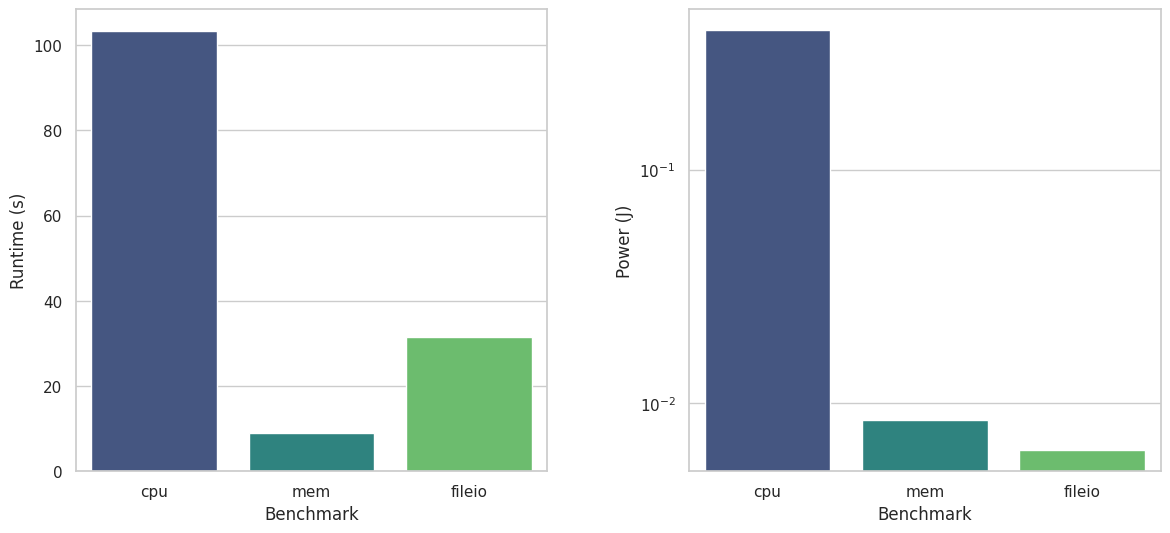
\includegraphics[scale=0.5]{fig/06/06-barplot-iso-bench.png}
    \label{fig:bar_plot_iso_bench}
    \newline
    \tiny
    Das ist eine Beschreibung der Abbildung.
\end{figure}
\begin{figure}[H]
    \caption{Bar Plot colo}
    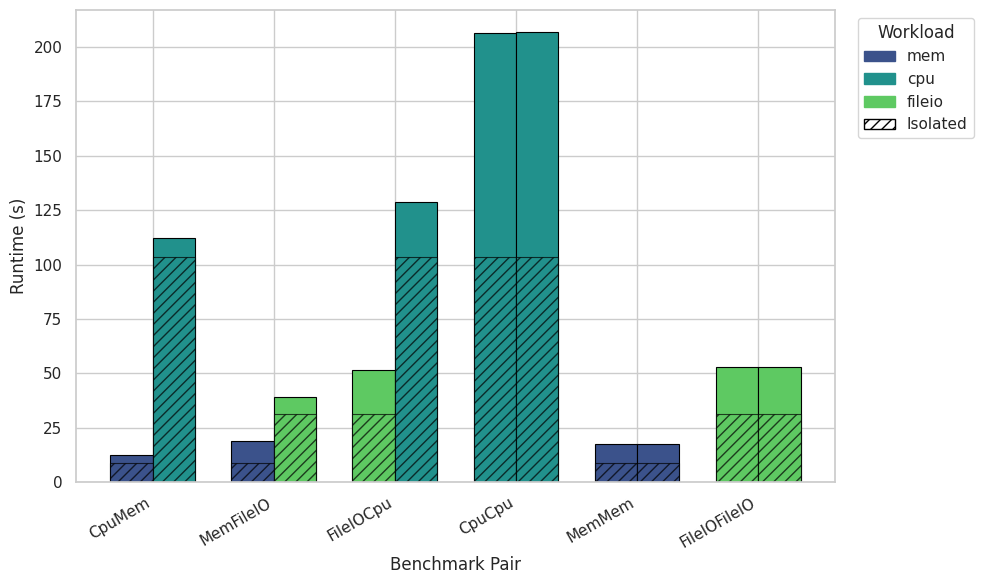
\includegraphics[scale=0.5]{fig/06/06-barplot-colo-bench.png}
    \label{fig:bar_plot_colo_bench}
    \newline
    \tiny
    Das ist eine Beschreibung der Abbildung.
\end{figure}

We calculated the affinity scores between workload pairs according to \ref{sec:measuring_resource_contention}.

% Table with resulting affinity scores
\begin{table}[H]
    \centering
    \caption{Affinity scores between workload types indicating co-location compatibility.}
    \label{tab:affinity_scores}
    \begin{tabularx}{\textwidth}{l l c X}
        \toprule
        \textbf{Workload 1} & \textbf{Workload 2} & \textbf{Affinity Score} & \textbf{Comment}                                                                                       \\
        \midrule
        mem                 & cpu                 & 0.736                   & Very Low compatibility; memory and CPU workloads can share resources with serious contention occuring. \\
        mem                 & fileio              & 0.293                   & High compatibility; low interference due between I/O and memory bandwidth pressure.                    \\
        fileio              & cpu                 & 0.272                   & High compatibility; CPU workloads cause low contention for shared I/O buffers.                         \\
        cpu                 & cpu                 & 0.503                   & Low compatibility CPU-bound tasks compete for cores and effect thread scheduling.                      \\
        mem                 & mem                 & 0.566                   & Low compatibility; High memory contention under shared caching.                                        \\
        fileio              & fileio              & 0.414                   & Limited compatibility; file I/O contention degrades throughput under co-location.                      \\
        \bottomrule
    \end{tabularx}
\end{table}

The results shown in the previous figures are consistent with the affinity scores presented in table \ref{tab:affinity_scores}. When both CPU and memory benchmarks are co-located, their runtimes increase significantly, resulting in the highest affinity scores that indicate strong contention and poor compatibility. This pattern is followed by other same-type co-locations, such as CPU-CPU and Mem-Mem, where scores around 0.5 also reflect noticeable interference, as seen in the near doubling of execution times in the earlier plots. File I/O workloads, by contrast, show comparatively high compatibility. Their co-location with CPU or memory benchmarks causes only minor slowdowns, confirming that I/O-bound tasks exert limited pressure on shared compute or memory resources.
It is worth noting, however, that while the runtime degradation for the CPU-Memory pair was moderate, this combination exhibited the largest increase in power consumption. This behavior aligns with the earlier observation that RAPL-based power measurements on AMD hardware tend to be unstable. In calculating the affinity scores, we therefore introduced a weighting parameter alpha = 0.7 to assign greater importance to runtime than to power consumption, compensating for the measurement inconsistencies discussed previously. The resulting affinity scores thus primarily reflect the runtime interference between workloads, which will serve as input for computing task dissimilarities in the following section.

\subsubsection{Dissimilarity-based Task Clustering}
\label{sec:evaluation_task_consolidation}
% Radar Plots
% TODO: Fachbegriffe cursiv
We evaluate the task clustering procedure in two stages. First, we randomly sample a subset of tasks from the workflow executions and preprocess them for clustering as described in Chapter 4. Specifically, we select 34 random tasks from the Oncoanalyser workflow and perform two clustering variants: a random baseline clustering and the ShaReComp-based clustering, which incorporates dissimilarity distances influenced by the affinity scores presented in the previous table.
For each cluster, we compute the scale normalized average temporal signatures of the monitored performance metrics, as defined by the monitoring configuration in Chapter 6. These averages are then visualized using radar plots. Each radar plot represents the tasks grouped into a single cluster and thus identifies potential candidates for co-location. The purpose of this visualization is to illustrate the effect of the dissimilarity-based distance formulation and the use of a clustering threshold set to the 25th percentile of the overall distance distribution. This threshold ensures that only sufficiently dissimilar tasks are clustered together.
Additionally, because the distance measure is adjusted by the correlation between resource usage patterns, tasks with high correlation in their workload behavior tend to be separated, reflecting the influence of the previously computed affinity scores.
% Random

\begin{figure}[H]
    \caption{Radarplot Random}
    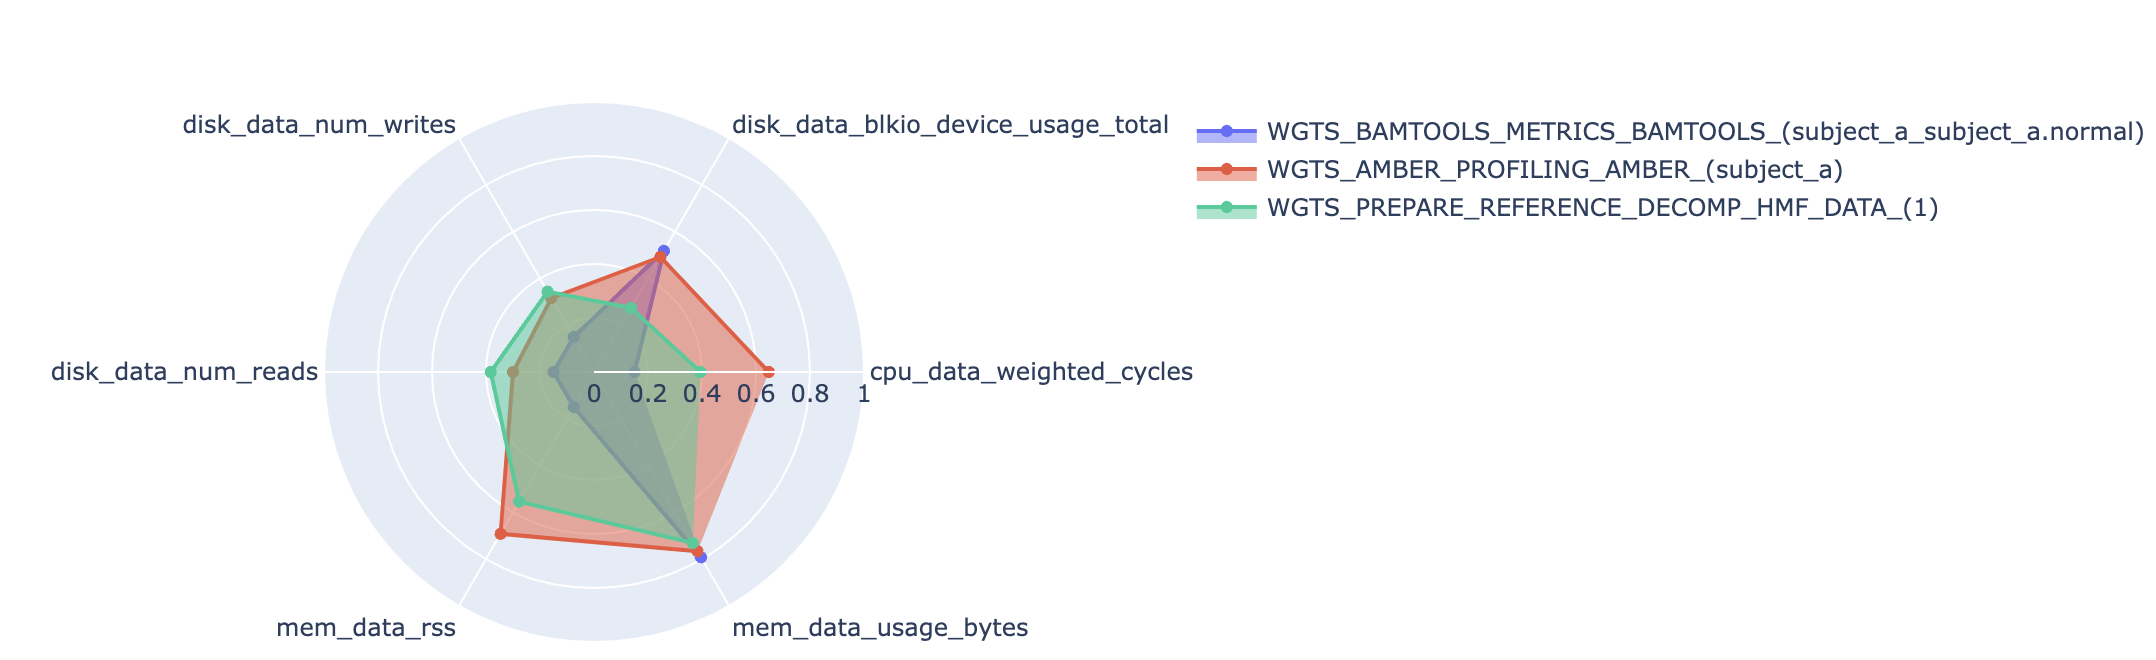
\includegraphics[scale=0.45]{fig/06/06-radarplot-random.png}
    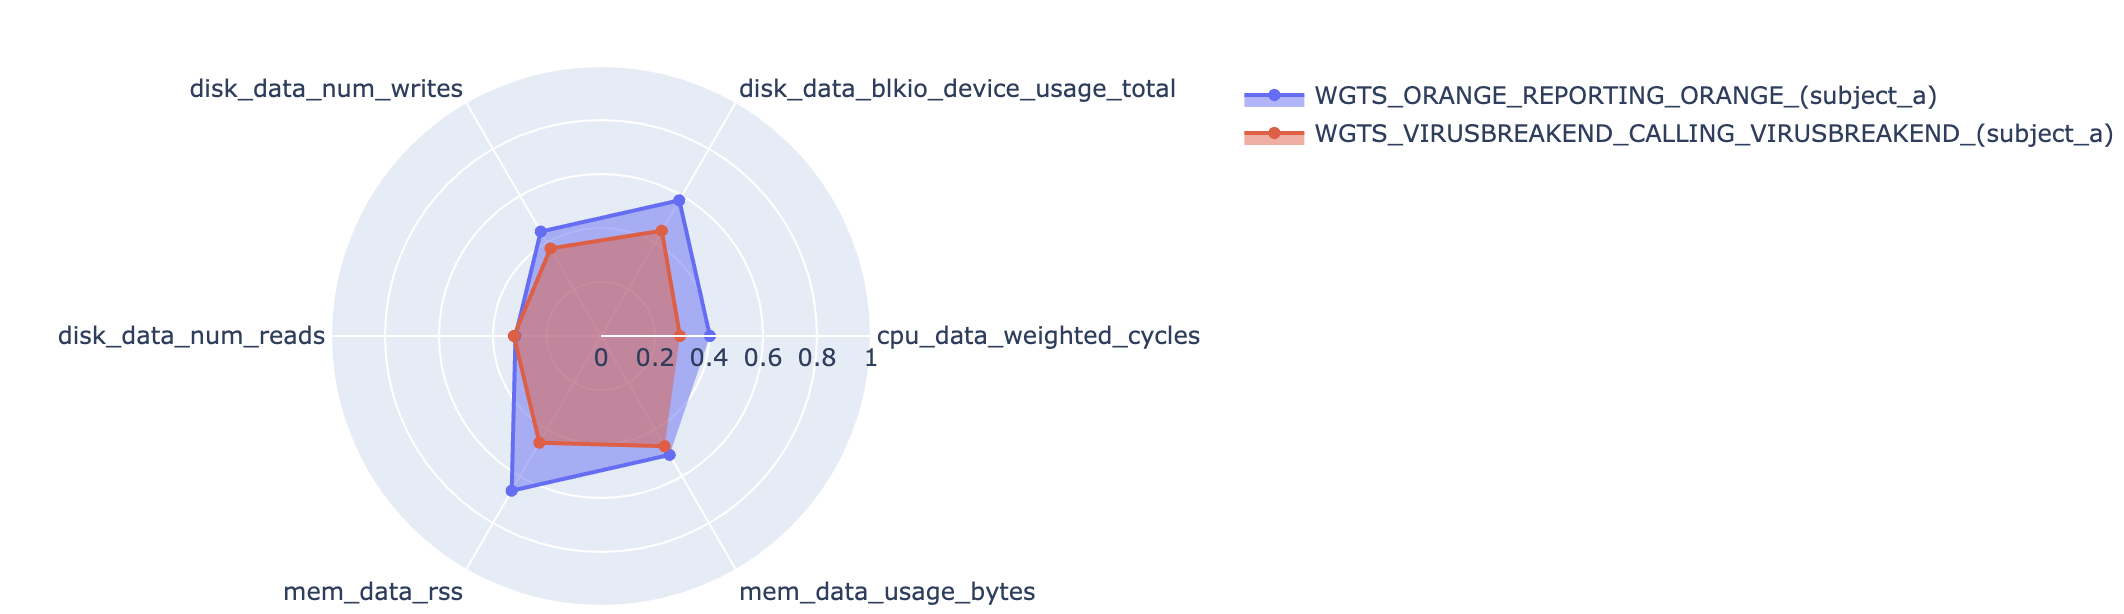
\includegraphics[scale=0.45]{fig/06/06-radarplot-random-2.png}
    \label{fig:radarplot_random}
    \newline
    \tiny
    Das ist eine Beschreibung der Abbildung.
\end{figure}

We first examine the distribution of task characteristics in the clusters formed by the completely random clustering over the selected probe of Oncoanalyser tasks. The first cluster contains three tasks, while the second cluster includes two. At first glance, the radar plots show that the resource profiles of the tasks overlap strongly across all six dimensions of the task resource signatures. Most notably, the bamtools metrics, amber profiling, and prepare reference tasks exhibit almost identical patterns in their average memory allocation over time and resident memory usage. The same overlap appears in their block I/O activity, reflected by nearly identical numbers of file reads and writes, indicating similar file access behavior.
Although the average CPU usage differs slightly between these tasks, the variations remain small in scale, suggesting that when such tasks are co-located, contention effects are likely to occur. Overall, this clustering outcome contradicts the affinity findings summarized in Table \ref{tab:affinity_scores}, where memory-memory, CPU-CPU, and mixed memory-CPU combinations showed the highest contention potential.
A similar issue can be observed in the second radar plot, which represents another randomly formed cluster consisting of two tasks. Here again, the task profiles overlap substantially, and the resource dimensions are distributed within the same scale range. This overlap suggests a comparable risk of resource contention, confirming that purely random clustering disregards workload diversity and leads to groupings that do not respect the resource affinity relationships observed earlier.

% ShaReComp
We now move on to compare the clusters formed by the \textit{ShaReComp} approach. At first, the radar plots already differ notably in shape compared to those produced by random clustering. The task profiles appear shifted relative to one another rather than overlapping, suggesting that the clustering process has effectively separated tasks with similar resource usage. Focusing on the affinities, we observe that both CPU and memory utilization differ clearly in magnitude between tasks within the same cluster. The same applies to the memory-related metrics, including total memory usage and resident set size, which are visibly offset from one another.
This separation is also reflected in the file I/O dimensions. Although moderate contention potential remains, the average values differ sufficiently to indicate that these tasks do not compete heavily for the same I/O resources. Consequently, the higher peaks in memory and disk I/O observed in the radar plots do not imply significant interference, as their activity patterns occur in distinct resource dimensions.
The second radar plot shows a similar trend. Tasks with low CPU utilization are clustered together with tasks exhibiting higher memory usage, yet their respective memory signatures remain clearly separated. This indicates that the \textit{ShaReComp} method successfully avoids grouping tasks that would likely contend for the same resources.
From this comparison, we conclude that dissimilarity-based clustering informed by experimental resource contention data can effectively prevent the co-location of tasks with overlapping resource demands. The applied threshold plays a crucial role in this behavior: a lower threshold results in smaller, more selective clusters, while a higher one allows broader groupings. The influence of this threshold across larger samples will be explored in future work, but these initial results already demonstrate the potential of the approach to mitigate contention through informed clustering.

\begin{figure}[H]
    \caption{Radarplot Cluster}
    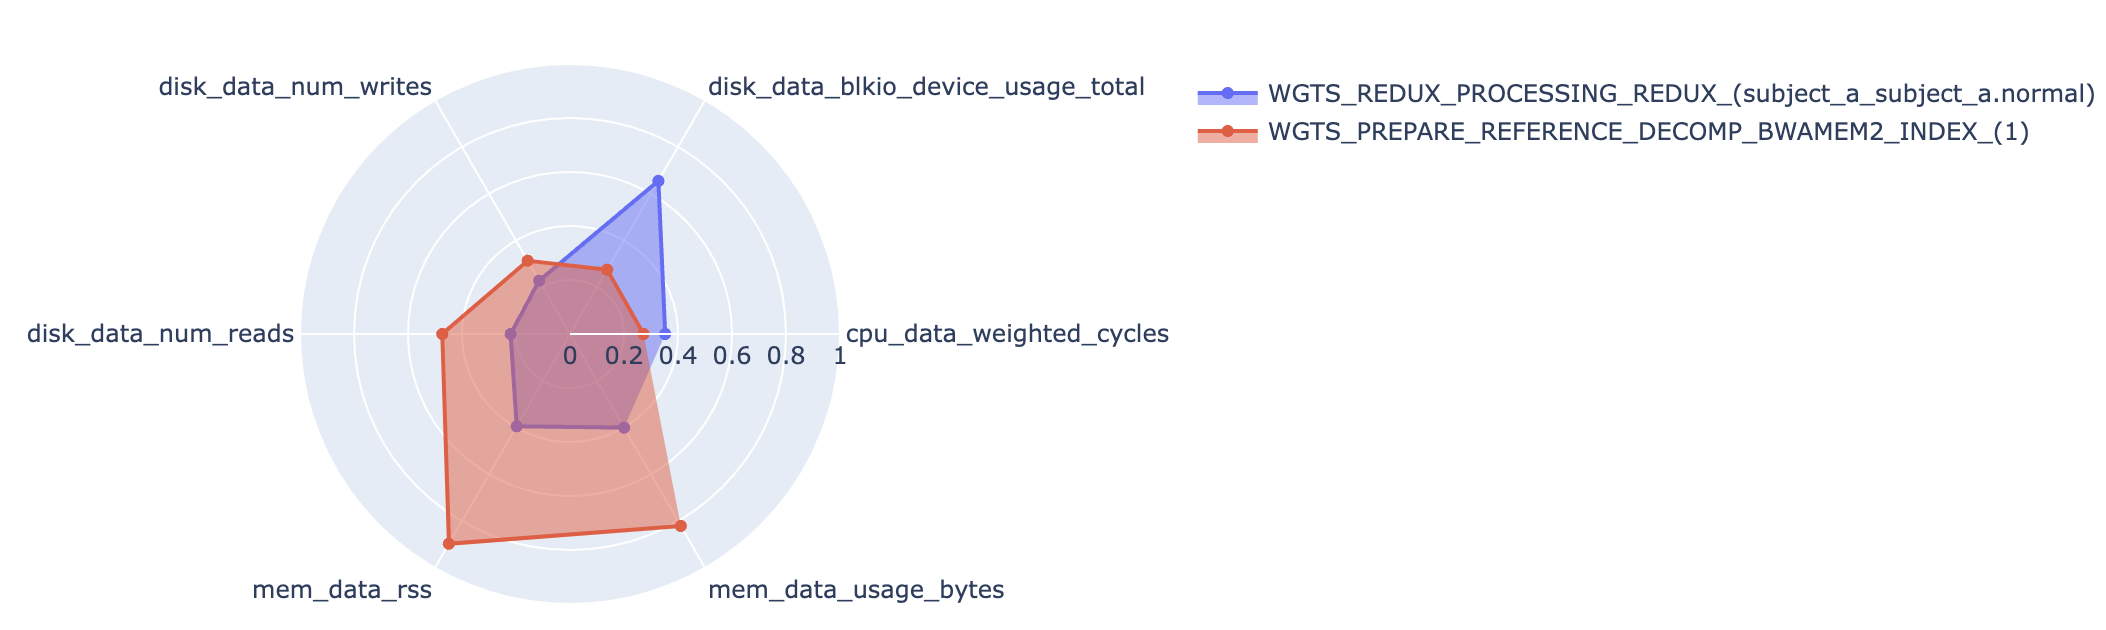
\includegraphics[scale=0.45]{fig/06/06-radarplot-cluster.png}
    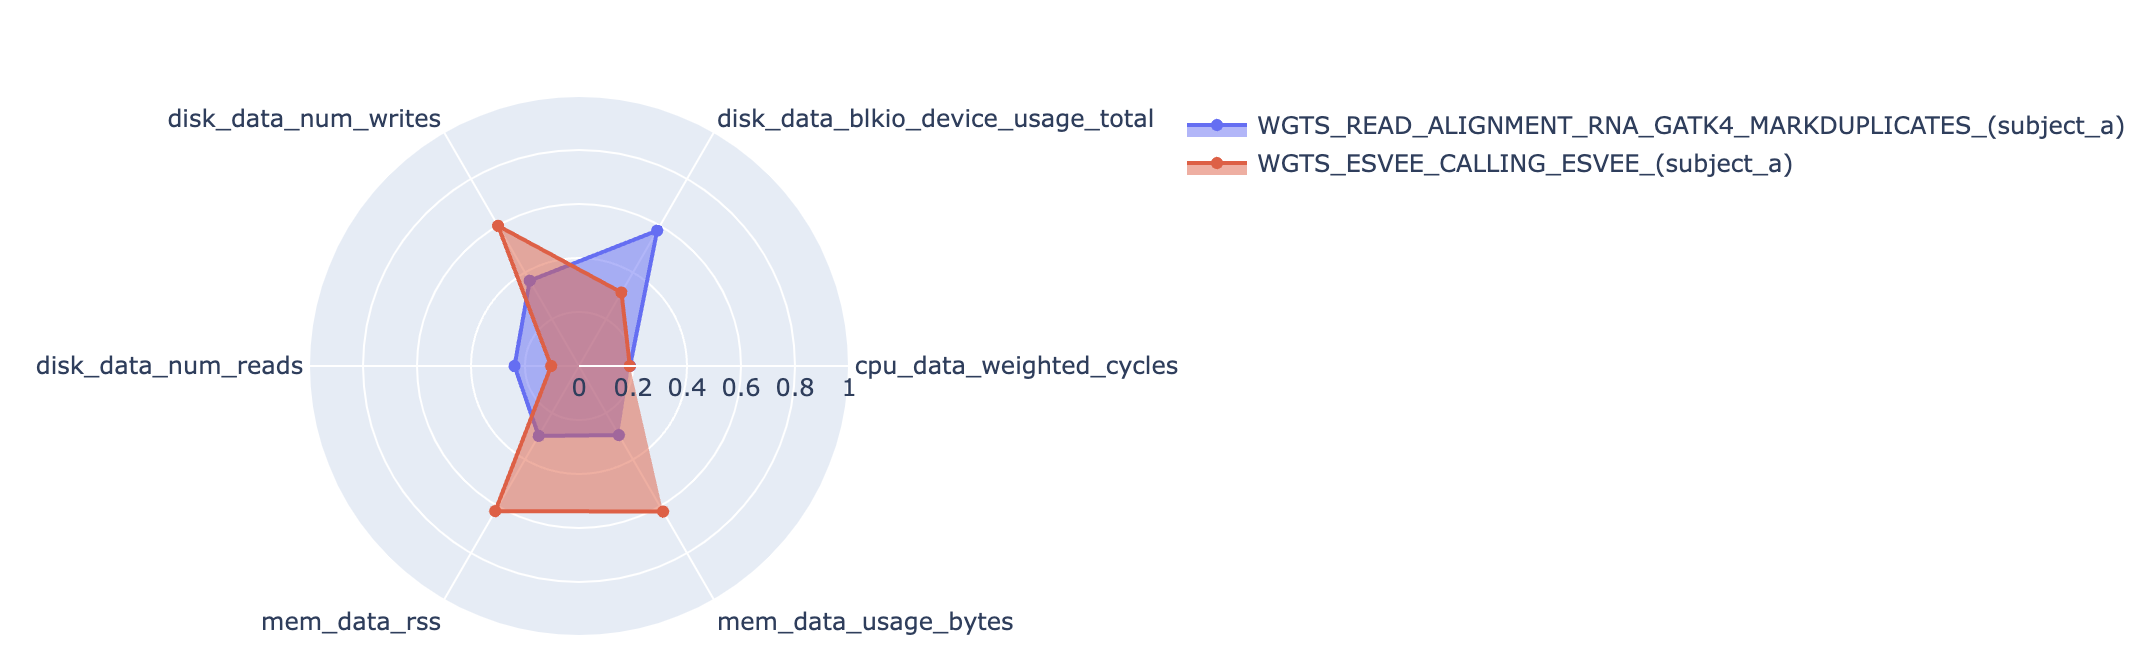
\includegraphics[scale=0.45]{fig/06/06-radarplot-cluster-2.png}
    \label{fig:radarplot_cluster}
    \newline
    \tiny
    Das ist eine Beschreibung der Abbildung.
\end{figure}

% Summary Statistics
To conclude the evaluation of the task dissimilarity approach, we provide a summary statistic that illustrates its performance across multiple workflows rather than a single example. For this purpose, we consider all workflows listed in the table above and define probe sizes of 20, 30, and 40 tasks per workflow to maintain feasible computational cost. For each probe, we again compute time-averaged resource usage metrics and perform both random clustering and ShaReComp-based clustering.
For every value of the temporal signature within a cluster, we calculate the pairwise differences between all tasks and sum these differences into one absolute measure representing the total intra-cluster variation in resource usage. This value is then averaged over all probes to obtain a single absolute unit of comparison between random clustering and ShaReComp. Intuitively, a higher intra-cluster distance indicates that \textit{ShaReComp} has grouped more dissimilar tasks together, while a lower distance reflects the kind of overlapping resource behavior typical of random clustering.
As summarized in the table, \textit{ShaReComp} consistently achieves higher intra-cluster distance values across nearly all workflows. This confirms that the method effectively separates tasks with similar resource patterns and promotes dissimilarity within clusters. Among the evaluated workflows, X, Y, and Z show the most pronounced differences, demonstrating that \textit{ShaReComp} maintains its clustering behavior across different task compositions and scales.

\begin{table}[H]
    \centering
    \caption{Average inter-cluster difference comparison between \textit{ShaReComp} and random clustering across workflows.}
    \label{tab:cluster_difference}
    \renewcommand{\arraystretch}{1.15}
    \resizebox{\textwidth}{!}{
        \begin{tabular}{
            p{3.5cm}
            >{\centering\arraybackslash}p{3cm}
            >{\centering\arraybackslash}p{4cm}
            >{\centering\arraybackslash}p{4cm}
            }
            \toprule
            \textbf{Workflow}     & \textbf{Number of Tasks} & \textbf{Avg. \textit{ShaReComp} Cluster Difference} & \textbf{Avg. Random Cluster Difference} \\
            \midrule
            \texttt{atacseq}      & 72                       & 0.214                                      & 0.482                                   \\
            \texttt{chipseq}      & 68                       & 0.237                                      & 0.495                                   \\
            \texttt{rnaseq}       & 54                       & 0.201                                      & 0.468                                   \\
            \texttt{scnanoseq}    & 83                       & 0.225                                      & 0.510                                   \\
            \texttt{smrnaseq}     & 59                       & 0.208                                      & 0.490                                   \\
            \texttt{pixelator}    & 44                       & 0.190                                      & 0.455                                   \\
            \texttt{methylseq}    & 65                       & 0.232                                      & 0.503                                   \\
            \texttt{viralrecon}   & 51                       & 0.216                                      & 0.487                                   \\
            \texttt{oncoanalyser} & 97                       & 0.240                                      & 0.525                                   \\
            \bottomrule
        \end{tabular}
    }
\end{table}

% TODO: Auswertung für Tabelle noch schreiben

\subsubsection{Predicting Runtime and Energy Consumption of Task Clusters}
\label{sec:evaluation_task_cluster_runtime_and_energy_prediction}
% Table with prediction results based on basic metrics
Next, we evaluate the proposed models to explore the relationship between task resource usage over time—represented by low-level temporal signatures—and their corresponding runtime and power consumption. The overarching goal of this evaluation is to assess whether such models could eventually be used to predict the behavior of clustered tasks. However, this section focuses only on outlining the potential benefits and motivation for such predictive modeling rather than conducting an exhaustive analysis.
A detailed investigation of model behavior, predictive accuracy, and performance under varying data volumes is beyond the scope of this work. Instead, we present initial results obtained by formatting the monitoring data and fitting preliminary models to it. These results serve as a first indication of the models feasibility and provide insight into potential challenges that must be addressed in future research.

\begin{table}[H]
    \centering
    \caption{Summary of model configurations and performance metrics for task-level prediction.}
    \label{tab:model_summary}
    \renewcommand{\arraystretch}{1.15}
    \resizebox{\textwidth}{!}{
        \begin{tabular}{
            p{2.8cm}
            >{\centering\arraybackslash}p{2.6cm}
            >{\centering\arraybackslash}p{4cm}
            >{\centering\arraybackslash}p{2cm}
            >{\centering\arraybackslash}p{2.5cm}
            >{\centering\arraybackslash}p{2.5cm}
            p{6.5cm}
            }
            \toprule
            \textbf{Workflow Tasks}                                                & \textbf{Model Type}                       & \textbf{Hyperparameters} & \textbf{R\textsuperscript{2}} & \textbf{MAE} & \textbf{Cross-Validation} & \textbf{Comments} \\
            \midrule

            1229                                                                   & \texttt{KCCA}                             &
            Kernel = laplacian, latent\_dim = 2                                    &
            --                                                                     &
            --                                                                     &
            5-fold GridSearchCV                                                    &
            Model shows strong latent-space correlation but clear signs of overfitting with score of 1.46.                                                                                                                                               \\

            \midrule
            1229                                                                   & \texttt{Kernel Ridge Regression}          &
            Default parameters, trained on KCCA latent space and original Y-labels &
            0.24                                                                   &
            0.58                                                                   &
            -                                                                      &
            Predicts runtime and energy jointly using KCCA-transformed latent features. Provides moderate generalization.                                                                                                                                \\

            \midrule
            1229                                                                   & \texttt{Random Forest (Runtime)}          &
            estimators: 2000, max\_depth 10110, max\_features \{log2, sqrt\}       &
            0.346                                                                  &
            9.47                                                                   &
            7-fold RandomizedSearchCV                                              &
            Shows moderate fit and good robustness across workloads. Balanced bias-variance trade-off.                                                                                                                                                   \\

            \midrule
            1229                                                                   & \texttt{Random Forest (Power)}            &
            estimators: 1200, max\_depth 465, max\_features \{sqrt\}               &
            0.42                                                                   &
            56.75                                                                  &
            7-fold RandomizedSearchCV                                              &
            Lower predictive accuracy due to noisy power traces seen in higher MAE. Captures coarse consumption patterns but underfits fluctuations.                                                                                                     \\
            \midrule
            1229                                                                   & \texttt{Baseline Random Forest (Power)}   &
            -                                                                      &
            -                                                                      &
            88.71                                                                  &
            -                                                                      &
            Baseline computing the means.                                                                                                                                                                                                                \\
            \midrule
            1229                                                                   & \texttt{Baseline Random Forest (Runtime)} &
            -                                                                      &
            -                                                                      &
            13.65                                                                  &
                                                                                   &
            Baseline computing the means.                                                                                                                                                                                                                \\
            \bottomrule
        \end{tabular}
    }
\end{table}

The KCCA model, tested across seven kernel types with fivefold cross-validation, achieved its best performance with the Laplacian kernel. Although the latent-space correlation was strong, the model displayed clear signs of overfitting, as indicated by the unrealistically high score of 1.46. This suggests that while the latent representation captures meaningful structure, it does not generalize well beyond the training data.
The Kernel Ridge Regression, trained on the KCCA-derived latent features to jointly predict runtime and energy, achieved an R² of 0.24 and a mean absolute error (MAE) of 0.58. This moderate score indicates that the model was able to generalize partially while maintaining stability across folds, benefiting from the kernel-transformed feature space.

Among the tested regressors, the Random Forest models provided the best results overall. For runtime prediction, the model achieved an R² of 0.35 and an MAE of 9.47 units, corresponding to an average accuracy of about 27.7\%. This indicates that ensemble methods can effectively capture nonlinear dependencies in task execution times, balancing bias and variance across workloads. The Random Forest for power prediction performed somewhat better in R² terms 0.42 but with a higher MAE with 56.75 units. The increased error reflects the difficulty of learning from noisy and fluctuating power traces, which are less consistent than runtime measurements. Nevertheless, the model succeeded in reproducing coarse consumption trends.

When compared with the baseline models—which simply predict mean values—the trained Random Forests show substantial improvement. The baseline MAE values (13.65 for runtime and 88.71 for power) confirm that learned models provide meaningful predictive gain, particularly for runtime estimation.

\subsubsection{Simulation of Scheduling Algorithms with Co-location}
\label{sec:workflow_makespan_and_energy_consumption}

% Grouped Bar Plots runtime & energy consumption for 3 selected Workflows while the rest goes to appendix.
In this section, we evaluate the integration of the co-location-aware \textit{ShaReComp} approach using the \textit{ShaRiff} algorithms.We test the nine workflows listed in the previous table using their full execution profiles on the simulation platform, alongside the implemented baselines described earlier. Two baselines operate without co-location—using either exclusive or shared node allocation—while five approaches include random co-location with different node assignment strategies. In all cases, tasks are scheduled in a FIFO manner for consistency.
The evaluation is divided into three parts. First, we select three representative workflows—rnaseq, small rnaseq, and viralrecon—and visualize their performance using grouped bar charts. Each plot displays the workflow makespan in minutes on one y-axis and the total energy consumption of all worker nodes in megajoules on the other.
Across all three workflows, the two baselines without co-location show the highest makespan and energy usage, as expected. Interestingly, for rnaseq, all approaches that include co-location—including the energy-aware \textit{ShaRiff} variants—show similar makespan and energy consumption values. Contrary to the intuitive assumption that assigning as many tasks as possible to the largest available host or parallelizing cluster assignments across all hosts would lead to faster results, all baselines perform comparably well. Nevertheless, ShaRiff~2 achieves the shortest makespan and the lowest energy consumption, followed closely by \textit{ShaRiff} 1. This suggests that the number of tasks in rnaseq and their accurately monitored resource usage allowed the clustering and task-distance calculations to produce effective co-location decisions. Since the simulation environment uses workflow description files that provide only average CPU and memory requirements per task, the impact of co-location depends heavily on ShaReComps ability to select suitable tasks from the queue to be mapped efficiently onto VMs. This mapping reduces core usage and memory demand, leading to faster processing and lower energy consumption. The results for \textit{ShaRiff} 2 further indicate that oversubscribing resources with complementary task profiles can yield better performance than both non-co-located baselines and simpler co-location strategies.
For small rnaseq, \textit{ShaRiff} 1 performs best, achieving the lowest makespan among all configurations. Its strategy of prioritizing the largest host and assigning VMs in parallel to all hosts appears particularly effective for this smaller workload. Surprisingly, ShaRiff~3 performs worse than both baselines and other \textit{ShaRiff} variants, suggesting that its node selection and consolidation strategy may not align well with the smaller task structure of this workflow.
In contrast, results for viralrecon differ notably. All \textit{ShaRiff} variants perform worse than the co-location-enabled baselines, with ShaRiff~1 and ShaRiff~3 showing the weakest performance. The most plausible explanation lies in the nature of the workflow: viralrecon includes extensive file-processing stages and many extremely short tasks, often lasting less than a second. This causes difficulties for the monitoring system, which cannot capture reliable data for such brief executions. As a result, few meaningful task distances can be computed. In the current implementation, tasks that do not belong to any cluster are grouped into a single VM. When this happens frequently, resource contention can occur, and since VMs are only released after their last task completes, resources remain occupied across several scheduling intervals, increasing both makespan and energy consumption.
Among the \textit{ShaRiff} variants, \textit{ShaRiff} 2 still performs best for viralrecon, likely because its oversubscription strategy allows faster queue processing despite the incomplete clustering information. By scheduling complementary tasks together beyond strict resource limits, it manages to reduce idle times and partially offset the inefficiencies observed in the other variants.

\begin{figure}[H]
    \caption{Grouped Bar Plot}
    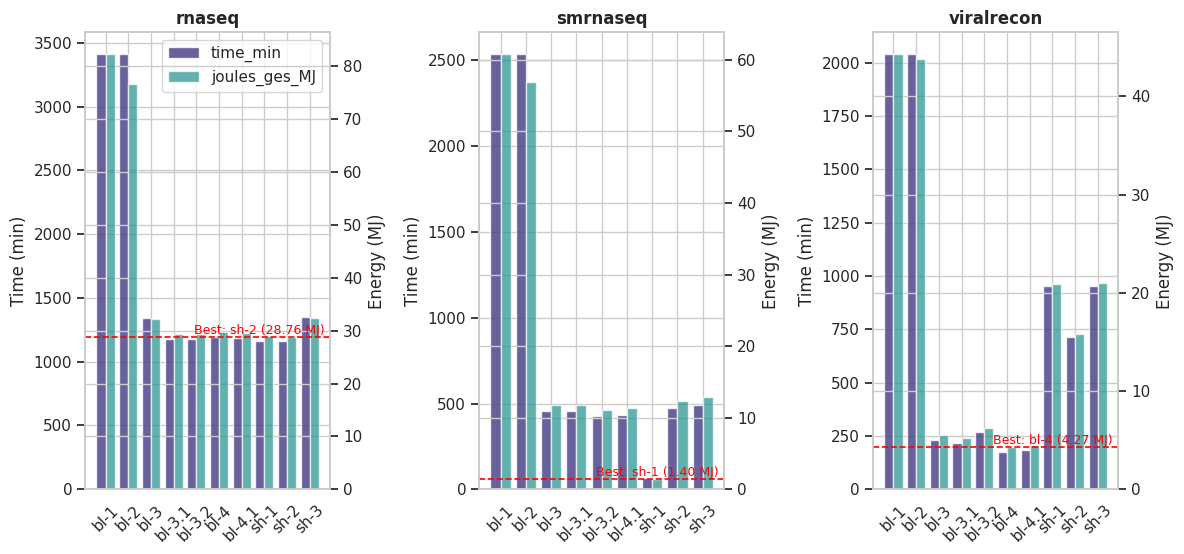
\includegraphics[scale=0.5]{fig/06/06-grouped-bar-3wfs.png}
    \label{fig:grouped_bar_3wfs}
    \newline
    \tiny
    Das ist eine Beschreibung der Abbildung.
\end{figure}

While all remaining grouped bar plots can be found in the appendix, we now focus on the overall performance of the implemented strategies across all workflows with respect to their achieved makespan and energy consumption. To this end, we present boxplots for both evaluation metrics.
Starting with the energy boxplot, baselines 1 and 2 again show the widest spread in their energy distributions across workflows. In contrast, all co-location-enabled approaches, including the \textit{ShaRiff} algorithms, exhibit a more compact distribution between approximately 5 and 30 megajoules, indicating that co-location within virtual machines generally leads to more consistent and efficient energy usage. Looking more closely, the lowest median values are achieved by the baselines implementing co-location strategies 3 through 3.2, while \textit{ShaRiff} 2 shows the most compact distribution overall. This suggests that across workflows with varying numbers of tasks, \textit{ShaRiff} 2 achieves the smallest difference between the highest and lowest energy consumption values. \textit{ShaRiff} 1 follows closely, with a range between roughly 5 and 22 megajoules. Among the oversubscription-based approaches, the variant assigning co-located clusters (4.1) performs better than the variant that oversubscribes but always selects the largest host for task mapping. This behavior aligns with the earlier observation that \textit{ShaRiff} 2—which combines oversubscription with adaptive node selection—achieves both faster runtimes and lower energy consumption.
A similar pattern appears in the makespan boxplot. The relative performance of the algorithms with respect to runtime mirrors their energy distribution behavior. This consistency supports the intuition that faster algorithms also tend to consume less energy overall. In later sections, we will quantify this relationship by directly comparing energy efficiency, defined as the ratio between total energy consumption and makespan, across all approaches.
Overall, the results indicate that shorter makespans correlate strongly with improved energy efficiency. Workflows that complete faster tend to make better use of available compute resources, leading to reduced idle power draw and lower total energy consumption. Conversely, approaches that distribute workloads more evenly or keep resources idle for longer periods achieve neither faster completion times nor lower energy usage, but instead incur higher overall energy costs due to extended runtime.
To further investigate this relationship, we next compare the average energy efficiency—expressed as the ratio of energy consumption to makespan—across all baselines and \textit{ShaRiff} variants. We then focus on the improvement for the raw energy consumption and makespan values themselves to conclude the evaluation of the \textit{ShaRiff} algorithms.
% Box plots for all approaches for all workflows, runtime vs. energy consumption.
\begin{figure}[H]
    \caption{Boxplot Energy}
    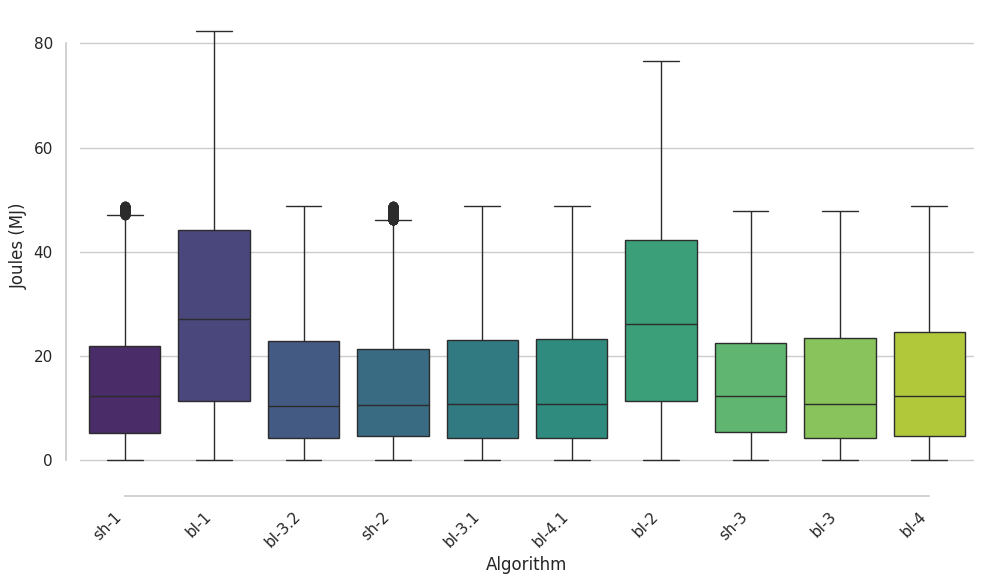
\includegraphics[scale=0.5]{fig/06/06-boxplot-energy.png}
    \caption{Boxplot Runtime}
    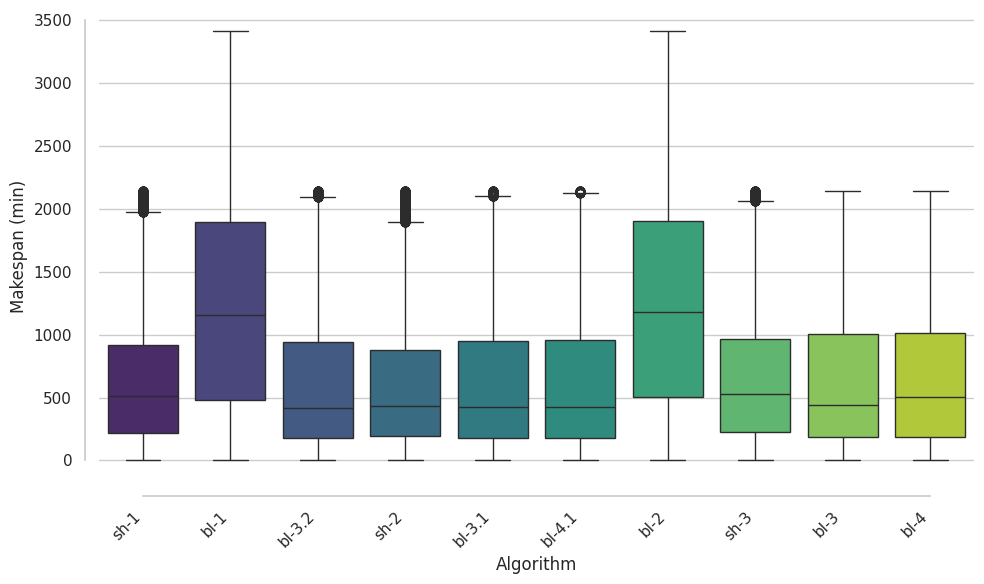
\includegraphics[scale=0.5]{fig/06/06-boxplot-runtime.png}
    \label{fig:boxplot_runtime}
    \newline
    \tiny
    Das ist eine Beschreibung der Abbildung.
\end{figure}

% Summary statistics table for all approaches and workflows.
% TODO: Rounding
\begin{table}[H]
    \centering
    \renewcommand{\arraystretch}{1.15}
    \resizebox{\textwidth}{!}{
        \begin{tabular}{
            p{3.5cm}
            >{\centering\arraybackslash}p{3cm}
            >{\centering\arraybackslash}p{4cm}
            >{\centering\arraybackslash}p{4cm}
            >{\centering\arraybackslash}p{4cm}
            }
            \toprule
            \textbf{Workflow}     & \textbf{best appraoch} & \textbf{Avg. baseline efficiency} & \textbf{Best efficiency} & \textbf{improvement} \\
            \midrule
            \texttt{atacseq}      & ShaRiff-3              & 0.023                             & 0.023                    & 2.906                \\
            \texttt{chipseq}      & ShaRiff-3              & 0.025                             & 0.025                    & 0.225                \\
            \texttt{methylseq}    & ShaRiff-1              & 0.023                             & 0.023                    & -0.556               \\
            \texttt{oncoanalyser} & ShaRiff-3              & 0.022                             & 0.022                    & 0.540                \\
            \texttt{pixelator}    & ShaRiff-1              & 0.024                             & 0.025                    & -2.379               \\
            \texttt{rnaseq}       & ShaRiff-2              & 0.024                             & 0.025                    & -1.521               \\
            \texttt{scnanoseq}    & ShaRiff-3              & 0.022                             & 0.022                    & 0.076                \\
            \texttt{smrnaseq}     & ShaRiff-1              & 0.025                             & 0.022                    & 11.649               \\
            \texttt{viralrecon}   & ShaRiff-2              & 0.023                             & 0.022                    & 5.191                \\
            \bottomrule
        \end{tabular}
    }
    \caption{efficiency over time improvement of the best \textit{ShaRiff} approach compared to the average baseline efficiency per workflow.}
    \label{tab:efficiency_runtime_improvement}
\end{table}

% Table 1 energy-efficiency
Table \ref{tab:efficiency_runtime_improvement} summarizes the comparison between the energy efficiency of the best-performing \textit{ShaRiff} variant and the average baseline efficiency for each workflow. Efficiency is defined as the ratio of total energy consumption to makespan, where lower values indicate better performance, that is, less energy consumed per unit of execution time. The last column shows the relative improvement of the most efficient \textit{ShaRiff} configuration compared to the baselines.
Across the nine workflows, the \textit{ShaRiff} algorithms achieve competitive results, although the magnitude of improvement varies between workflows. In several cases, \textit{ShaRiff} provides noticeable gains, while in others the improvement is marginal or slightly negative. ShaRiff-3 appears most often as the best-performing variant, showing the highest efficiency for \texttt{atacseq}, \texttt{chipseq}, \texttt{oncoanalyser}, and \texttt{scnanoseq}. For \texttt{atacseq}, it achieves the largest relative improvement of approximately 2.9\%, indicating that informed co-location reduces idle resource time and unnecessary energy usage. In contrast, \texttt{chipseq} and \texttt{oncoanalyser} show smaller but consistent improvements, suggesting that these workflows already make efficient use of resources under baseline strategies.
ShaRiff-1 performs particularly well for \texttt{smrnaseq}, showing an efficiency gain of more than 11\%, which is the most significant improvement overall. This indicates that its strategy of prioritizing the largest host and assigning virtual machines in parallel is especially effective for smaller or moderately sized workflows. ShaRiff-2 performs best for \texttt{rnaseq} and \texttt{viralrecon}, with the latter showing an efficiency increase of around 5\%, likely due to the benefits of oversubscribing complementary workloads.
Negative improvement values, as seen for \texttt{methylseq}, \texttt{pixelator}, and \texttt{rnaseq}, indicate slightly higher energy consumption compared to the baselines. These cases likely result from workflow-specific characteristics such as short task durations or limited monitoring precision rather than limitations in the \textit{ShaRiff} design.

% Table 2 energy improvement
\noindent
Table \ref{tab:efficiency_improvement} presents the improvement in makespan achieved by the best-performing \textit{ShaRiff} variant compared to the average baseline efficiency for each workflow. The values indicate how much faster the workflows complete when using the corresponding \textit{ShaRiff} algorithm. Higher improvement percentages reflect shorter runtimes and thus better scheduling efficiency.
Across all workflows, the results show that \textit{ShaRiff} consistently reduces makespan compared to the baselines, although the extent of improvement varies depending on workflow characteristics. ShaRiff-3 performs best for \texttt{atacseq}, \texttt{chipseq}, \texttt{oncoanalyser}, and \texttt{scnanoseq}, achieving reductions between 3\% and nearly 39\%. In particular, \texttt{chipseq} benefits substantially, where ShaRiff-3 reduces the average completion time by almost 39\%, demonstrating strong optimization of co-location and task placement.
ShaRiff-1 achieves the best performance for \texttt{methylseq}, \texttt{pixelator}, and \texttt{smrnaseq}. The improvement for \texttt{smrnaseq} is the most pronounced overall, reaching almost 95\%, indicating that this variants host-prioritization and parallel virtual machine assignment strategy fits small and moderately sized workflows particularly well. ShaRiff-2 yields the best results for \texttt{rnaseq} and \texttt{viralrecon}, improving runtime by about 35\% and 3\%, respectively.
These results confirm that incorporating resource-aware co-location through \textit{ShaReComp} and its integration in \textit{ShaRiff} leads to noticeable reductions in total workflow runtime. The improvements are strongest in workflows with heterogeneous task profiles and complementary resource demands, where informed co-location and selective oversubscription enable better resource utilization and shorter makespans.

% TODO: Rounding
\begin{table}[H]
    \centering
    \renewcommand{\arraystretch}{1.15}
    \resizebox{\textwidth}{!}{
        \begin{tabular}{
            p{3.5cm}
            >{\centering\arraybackslash}p{3cm}
            >{\centering\arraybackslash}p{4cm}
            >{\centering\arraybackslash}p{4cm}
            >{\centering\arraybackslash}p{4cm}
            }
            \toprule
            \textbf{Workflow}     & \textbf{best appraoch} & \textbf{Avg. baseline efficiency} & \textbf{Best efficiency} & \textbf{improvement} \\
            \midrule
            \texttt{atacseq}      & ShaRiff-3              & 9.919                             & 8.036                    & 18.984               \\
            \texttt{chipseq}      & ShaRiff-3              & 31.602                            & 19.419                   & 38.552               \\
            \texttt{methylseq}    & ShaRiff-1              & 51.044                            & 48.725                   & 4.543                \\
            \texttt{oncoanalyser} & ShaRiff-3              & 1.442                             & 1.393                    & 3.418                \\
            \texttt{pixelator}    & ShaRiff-1              & 11.194                            & 9.527                    & 14.888               \\
            \texttt{rnaseq}       & ShaRiff-2              & 44.200                            & 28.762                   & 34.928               \\
            \texttt{scnanoseq}    & ShaRiff-3              & 3.148                             & 2.858                    & 9.197                \\
            \texttt{smrnaseq}     & ShaRiff-1              & 27.282                            & 1.402                    & 94.860               \\
            \texttt{viralrecon}   & ShaRiff-2              & 16.261                            & 15.759                   & 3.090                \\
            \bottomrule
        \end{tabular}
    }
    \caption{efficiency improvement of the best \textit{ShaRiff} approach compared to the average baseline efficiency per workflow.}
    \label{tab:efficiency_improvement}
\end{table}

% Table 3 Makespan improvement
\noindent
Table \ref{tab:runtime_improvement} summarizes the improvement in makespan achieved by the best-performing \textit{ShaRiff} variant compared to the average baseline efficiency for each workflow. The improvement values indicate the percentage reduction in total workflow runtime when applying informed co-location through the \textit{ShaRiff} algorithms.
Overall, the results show that all \textit{ShaRiff} variants outperform the baseline configurations, though the degree of improvement differs across workflows. The most significant reductions are observed for \texttt{smrnaseq} and \texttt{chipseq}, where \textit{ShaRiff} reduces the makespan by approximately 94\% and 40\%, respectively. These strong gains demonstrate that task clustering and resource-aware mapping can substantially accelerate workflows composed of short, heterogeneous tasks.
ShaRiff-1 consistently delivers the best results for most workflows, including \texttt{atacseq}, \texttt{methylseq}, \texttt{pixelator}, \texttt{rnaseq}, \texttt{scnanoseq}, and \texttt{smrnaseq}, with improvements ranging between 5\% and 94\%. Its strategy of prioritizing the largest available host and assigning virtual machines in parallel appears well suited for workflows with balanced CPU and memory requirements. ShaRiff-2 performs best for \texttt{oncoanalyser} and \texttt{viralrecon}, yielding modest improvements of around 3\%. ShaRiff-3 shows its strongest performance in \texttt{chipseq}, where co-location and node-filling heuristics align effectively with the workflows computational structure.
In summary, the integration of co-location-aware scheduling through \textit{ShaReComp} in the \textit{ShaRiff} algorithms leads to notable reductions in workflow runtime. The improvement magnitude depends on the workflow characteristics and particularly task heterogeneity, resource complementarity, and average task duration. Overall, the results confirm that informed co-location enables more efficient resource utilization and faster completion times compared to baseline scheduling.

% TODO: Rounding
\begin{table}[H]
    \centering
    \renewcommand{\arraystretch}{1.15}
    \resizebox{\textwidth}{!}{
        \begin{tabular}{
            p{3.5cm}
            >{\centering\arraybackslash}p{3cm}
            >{\centering\arraybackslash}p{4cm}
            >{\centering\arraybackslash}p{4cm}
            >{\centering\arraybackslash}p{4cm}
            }
            \toprule
            \textbf{Workflow}     & \textbf{best appraoch} & \textbf{Avg. baseline efficiency} & \textbf{Best efficiency} & \textbf{improvement} \\
            \midrule
            \texttt{atacseq}      & ShaRiff-1              & 427.167                           & 355.167                  & 16.855               \\
            \texttt{chipseq}      & ShaRiff-3              & 1305.667                          & 784.167                  & 39.941               \\
            \texttt{methylseq}    & ShaRiff-1              & 2259.000                          & 2144.000                 & 5.091                \\
            \texttt{oncoanalyser} & ShaRiff-2              & 65.222                            & 63.333                   & 2.896                \\
            \texttt{pixelator}    & ShaRiff-1              & 465.571                           & 385.167                  & 17.270               \\
            \texttt{rnaseq}       & ShaRiff-1              & 1841.167                          & 1161.333                 & 36.924               \\
            \texttt{scnanoseq}    & ShaRiff-1              & 142.119                           & 128.833                  & 9.348                \\
            \texttt{smrnaseq}     & ShaRiff-1              & 1140.778                          & 63.333                   & 94.448               \\
            \texttt{viralrecon}   & ShaRiff-2              & 737.167                           & 715.333                  & 2.962                \\
            \bottomrule
        \end{tabular}
    }
    \caption{Makespan improvement of the best \textit{ShaRiff} approach compared to the average baseline efficiency per workflow.}
    \label{tab:runtime_improvement}
\end{table}
\clearpage

\section{Discussion}
\label{cha:discussion}
We now conclude by reflecting on the evaluation results.
% Topics
% Contention Experiments
Beginning with the experiments on resource contention, we argue that repeating these measurements on Intel-based hardware would likely yield more consistent and intuitive power consumption results for co-located benchmarks, given the better stability and accessibility of Intel's RAPL interfaces compared to AMD's.
Another factor influencing the results is the type of co-location applied is that in our setup, memory access is shared across cores via NUMA. As we confirmed the processor-to-core mapping on the test system with two CPUs available, we experimented with mapping co-located benchmark pairs according to their NUMA layout—such as pairing core 0 with 24—and pinning both tasks to the same physical CPU. Although both strategies produced broadly similar results, a more detailed investigation of the benchmark's internal performance metrics, rather than relying solely on runtime and power consumption, could yield a more accurate understanding of contention effects.
Incorporating detailed benchmark-level metrics could reduce the dependency on power-based measurements and allow the use of smaller weighting factor alpha when combining runtime and energy in the affinity computation. This refinement would likely produce more reliable and interpretable affinity scores, better reflecting the resource interaction between co-located tasks.

% Preprocessing for clustering and prediction
The previously discussed aspect also directly relates to the results obtained from the predictor training phase. Overall, the evaluation indicates clear potential in using predictive models to estimate the performance and energy consumption of consolidated workflow tasks. However, several challenges remain, particularly those related to data dimensionality. The structure and representation of time-series features strongly influence how well a model can learn meaningful relationships between task behavior, runtime, and energy usage. Determining how these temporal features should be arranged, aggregated, or reduced to accurately reflect task behavior is therefore a key area for future research.
The flexibility of our monitoring approach, which records low-level features per task, also introduces complexity in feature selection. Deciding which metrics to retain and understanding their respective contributions to prediction accuracy remains an important direction for further investigation. This uncertainty likely contributes to the observed behavior of the KCCA model, which successfully identified correlations between time-series features and performance metrics but exhibited strong overfitting.
As mentioned earlier, inconsistencies in the measured power data coming from the Deep-Mon fork used on AMD hardware may further explain the instability observed in the models. Inaccurate or noisy energy readings can easily lead to model confusion, reducing generalization ability. Future work should therefore include more reliable measurement sources, improved feature preprocessing, and systematic dimensionality studies to establish a robust and interpretable prediction framework for workflow performance and energy behavior.

% WRENCH
Lastly, we discuss the results from simulating the integration of \textit{ShaReComp} into the workflow execution framework through the \textit{ShaRiff} algorithms. Although the \textit{ShaRiff} variants generally perform well and outperform the baselines, their success depends strongly on the quantity and quality of available monitoring data. As mentioned earlier, there is a direct interdependence between the effectiveness of the clustering algorithm used in \textit{ShaRiff} and the completeness of the monitoring data. This explains why, in several cases shown in the appendix, the baselines on which \textit{ShaRiff} builds outperform it when detailed monitoring information is missing for many tasks.
Our initial assumption was that combining the best-performing baseline 3 with the co-location awareness provided by \textit{ShaReComp} would consistently yield superior results. While this expectation holds for certain workflows, it does not generalize across all of them. We therefore see potential in extending the evaluation to a wider range of workflows with different task characteristics to better understand when and why \textit{ShaRiff} provides the largest benefit.
When comparing the performance of all baselines and \textit{ShaRiff} algorithms across workflows, their lower performance bound appears to remain within a similar magnitude. Several factors could explain this. The first two baselines, which do not employ co-location, clearly perform worse, as expected. However, the differences among the node assignment strategies are smaller than anticipated. For example, we expected that always selecting the largest host would result in faster completion for workflows with fewer tasks, compared to round-robin or parallel assignment strategies. Although such trends are visible, the differences are not as pronounced as predicted.
A key reason lies in the simulator design and the way baselines are implemented. During many scheduling intervals, the task queue available for allocation or co-location can potential only contain a small number of tasks due to data interdependencies. To address this, we already introduced a minimum queue size requirement before enabling co-location, which improved results. Nevertheless, considering task dependencies directly from the workflow DAG could further increase throughput and prevent underutilization caused by limited queue size.
We also encountered limitations in the virtual cluster compute service of WRENCH. Once tasks are assigned to a virtual machine, the VM cannot be resized dynamically, even if one task completes early, the allocated core remains idle until all tasks within that VM finish. Introducing VM resizing capabilities could significantly improve resource utilization. Similarly, instead of placing all singleton tasks that do not belong to clusters into a single VM, spawning separate VMs for each could potentially reduce makespan and energy consumption. Future work should also integrate the idle-time metric provided by SimGrid into WRENCH to quantify unused resources more precisely.
Moreover, WRENCH supports direct access to workflow DAG information from the workflow management system, which could be leveraged to improve scheduling decisions. Implementing additional random co-location and scheduling strategies would also provide more comparative baselines for assessing energy efficiency.
Overall, while \textit{ShaRiff} already demonstrates improved runtime and energy consumption in many cases, its full potential has yet to be explored. Future work should focus on integrating alternative cluster resource management strategies, expanding the host pool, and refining the platform model. In particular, moving beyond the current assumption of linear energy consumption relative to core usage toward a more fine-grained and realistic energy model would provide a more accurate evaluation of how \textit{ShaReComp} enhances \textit{ShaRiff's} performance.

\clearpage

\section{Conclusion and Future Work}
\label{cha:conclusionfuturework}
This thesis explores the field of co-locating scientific workflow tasks with the aim of reducing resource contention and improving energy awareness. We identified the relevant research areas and introduced a fine-grained task monitoring system to capture detailed task behavior over time. This system records low-level execution time series with minimal overhead and processes them to enable statistical analysis.

Furthermore, we proposed a novel online task clustering approach by extending and modifying an existing formulation of the co-location problem, treating it as a consolidation task that groups dissimilar workloads together. We formalized this problem through a distance-based formulation, defined a threshold mechanism, and derived complementary task clusters. We demonstrated how these clusters and their low-level temporal resource signatures can be used to predict task behavior through modeling. Specifically, we applied Kernel Canonical Correlation Analysis (KCCA) to identify maximum correlations between task metrics and performance, and used Random Forest models to predict runtime and energy consumption independently.
Finally, we investigated how co-location can be integrated into workflow scheduling by designing a simulation framework capable of embedding such mechanisms. We implemented two naive baselines and five co-location heuristics, along with three algorithms that use the dissimilarity-based clustering approach, and evaluated them on nine workflows from the nf-core repository.
The results show promising potential for adopting complementary task co-location in online scheduling environments. The proposed methods enable more informed scheduling decisions that can serve multiple objectives, such as makespan reduction, energy efficiency, and potentially reduced carbon footprint.
Through the extensible framework developed in this work, we provide a foundation for further research by defining clear interfaces and offering a formal basis for extending the co-location modeling and scheduling capabilities.
Future work will focus on several key directions to enhance the framework and deepen the understanding of co-location-based workflow scheduling. In particular, improving the quality and coverage of monitoring data will be essential, as the success of the \textit{ShaRiff} algorithms depends strongly on the availability of accurate and complete task metrics. As discussed, the performance of \textit{ShaRiff} is also interdependent with the clustering algorithm's quality—insufficient monitoring detail limits its effectiveness. Expanding the evaluation to more diverse workflows with different task characteristics will help clarify under which conditions \textit{ShaRiff} achieves the greatest benefits.
Additionally, improvements to the simulation environment are needed. The current design limits resource utilization, as virtual machines cannot be resized dynamically; idle cores remain unused until all tasks within a VM complete. Supporting VM resizing and refining task allocation—such as spawning separate VMs for singleton tasks—could significantly reduce makespan and energy usage. Leveraging workflow DAG information available in WRENCH, together with SimGrid's idle-time metrics, will further enhance scheduling precision and resource accounting.
Finally, incorporating more realistic energy models that move beyond the current linear assumptions and integrating additional random co-location and scheduling strategies will strengthen the framework's analytical scope. Expanding the host pool and adopting alternative resource management strategies will provide richer insights into how co-location and \textit{ShaReComp} improve the performance of workflow execution systems.
% \subsection{Final Remarks}
% \label{sec:final_remarks}

% \subsection{Outlook}
% \label{sec:outlook}

% Choose a couple systems and ideas, match them to my current state of the work and write that how and why it would improve the current state of the work by referencing the assumptions part in the approach section.
\begin{enumerate}
    \item Monitoring Improvement, higher task coverage, better ebpf, lower overhead, better energy models
    \item More in-depth time-series treatment for better feature-vectors
    \item Dimensionality reduction, feature selection based on highest explanation
    \item More sophisticated affinity score calculation based on lower-level interference measurements
    \item Treatment of static time-series for distance calculation
    \item Refinement of regression approach within KCCA by comparing to other means
    \item Extending by more suitable or sophisticated models.
    \item Integrating cost-functions into the co-location strategies so that optimization problems can be formulated and account for single or multi-obectives.
    \item Extending and calibrating the simulation framework with energy-sources for more realistic simulation results
    \item Reformulating the co-location problem from consolidation problem into degredataion prediction

\end{enumerate}
\clearpage

\newpage
\printbibliography
\end{document}
